\documentclass[a4paper, twoside, titlepage]{book}

\usepackage[T1]{fontenc}
\usepackage[utf8]{inputenc}
\usepackage[italian]{babel}

\usepackage{microtype}
\usepackage{xcolor}
\usepackage{titlesec}
\usepackage{xargs}
\usepackage{multicol}
\usepackage{amsmath}
\usepackage{amssymb}
\usepackage{quoting}
\quotingsetup{font=small}

\usepackage{ulem}
\usepackage{framed}
\usepackage{amsmath}
\usepackage{graphicx}

\DeclareUnicodeCharacter{200B}{{\hskip 0pt}}

%definizioni particolari
\newcommand{\straniero}[1]{\textit{#1}} %parole straniere
\newcommand{\titolo}[1]{\textsc{#1}} %titoli
\newcommand{\evid}[1]{\textbf{\textcolor{blue}{#1}}} %parole evidenziate
\newcommand{\salt}{\hspace{1em}[...]} %comando per la creazione dei puntini di sospensione tra quadre
%

%citazioni
\newcommand{\citazione}[1]{%
  \begin{quotation}
  #1
  \end{quotation}}
%

%definire header e footer
\usepackage{fancyhdr}
\pagestyle{fancy}

\fancyhf{}
\fancyhead[LE,RO]{\scshape\thepage}
\fancyhead[LO]{\scshape\footnotesize\nouppercase{\rightmark}}
\fancyhead[RE]{\scshape\footnotesize\nouppercase{\leftmark}}
%

%rimuovere header e footer dalle pagine vuote
\makeatletter
\def\cleardoublepage{\clearpage\if@twoside \ifodd\c@page\else
    \hbox{}
    \vspace*{\fill}
    \vspace{\fill}
    \thispagestyle{empty}
    \newpage
    \if@twocolumn\hbox{}\newpage\fi\fi\fi}
\makeatother
%

\renewcommand{\emph}[1]{\textcolor{blue}{#1}}

%%%%%% HYPERREF VA CARICATO SEMPRE PER ULTIMO, DEMENTE!

\usepackage[colorlinks, pdftex, pdfauthor={Davide Peccioli},
            pdftitle={Riepilogo Filosofia},
            pdfsubject={Da Kant a Nietzsche}]{hyperref}
\definecolor{RoyalBlue}{rgb}{0.0, 0.14, 0.4}
\hypersetup{
     colorlinks=true,
     linkcolor=blue,
     filecolor=blue,
     citecolor = black,
     urlcolor=cyan,}

\title{Filosofia}
\author{Davide Peccioli}
\date{a.s. 2020-2021}

\begin{document}

\begin{titlepage} % pagina del titolo
\begin{center}
    \null
    \vfill
    {\huge \textsc{Appunti di Filosofia}}\\
    \vspace{2em}
    {\Large Da Kant a Nietzsche}\\
    \vspace{3em}
    {\large \textbf{Davide Peccioli}}\\
    \vspace{1em}
    {\large Classe 5\textsuperscript{a}\\\vspace{0.4em} a.s. 2020-2021}
    \fancyfoot[C]{}
    \vfill
\end{center}
\end{titlepage}
\tableofcontents

\part{Kant}

\chapter*{Introduzione}

Empirismo e razionalismo non sono tra di loro in contraddizione, ma entrambe utilizzano sia ragione che esperienza: cambiano solo le proporzioni. In caso di conflitto, gli empiristi preferiranno l’\textbf{esperienza}, mentre i razionalisti preferiranno la \textbf{ragione}.

\textbf{Kant} è un filosofo che viene alla fine dell’\textbf{illuminismo}, ovvero un periodo caratterizzato dalla ragione. Il suo obiettivo è quello di portare la \textit{ragione} di fronte al tribunale della ragione stessa, cercando di capirne limiti e funzioni.
Pertanto mette sullo stesso piano ragione ed esperienza, cercando di capire quale sia il migliore approccio alla realtà stessa.

Noi partiremo dall’analisi dei \textit{giudizi}. Un giudizio è una affermazione in cui si aggiunge un predicato ad un soggetto.
I giudizi possono essere di due tipi:
\begin{enumerate}
\item \textbf{Giudizi analitici a priori}: è un giudizio che tende ad analizzare su base razionale l’oggetto della conoscenza; è il tipo di giudizio maggiormente espresso dai razionalisti: non partono dall’esperienza ma dall’analisi razionale
È un giudizio a cui si può pervenire ragionando, senza passare dall’esperienza
Il termine \textit{a priori} significa anche “universale e necessario”, poiché è valido in ogni tempo e ogni luogo.
\emph{La loro forza sta proprio nel loro carattere di universalità e validità perenne.}
\item \textbf{Giudizio sintetico a posteriori}: è un giudizio che esprime il risultato di una esperienza.  È legato ad un \textit{qui} e un \textit{ora}. Questo giudizio non è universale e necessario, poiché non è valido in ogni tempo e in ogni luogo. È un giudizio \textit{sintetico} perché esprime una sintesi di dati che provengono dai miei organi di senso. 
Sono \textbf{fecondi}, perché dicono qualcosa in più rispetto a ciò che già sapevo per mezzo della ragione.
\emph{Il loro punto di forza è che danno delle informazioni in più rispetto ad un ragionamento di tipo unicamente razionale.}
\end{enumerate}

Kant vuole pervenire ad un punto di unione tra questi due giudizi, in modo da unire i punti di forza di entrambi i tipi di conoscenza.

Kant si pone, quindi, la domanda:

\emph{Esistono dei giudizi sintetici a priori?}

Questa è la domanda su cui si basa tutta la sua analisi, svolta nel libro \textbf{Critica della ragion pura}.
Egli infatti cerca di coniugare i lati positivi di entrambi i giudizi

Egli scrive altre opere:
\begin{enumerate}
\item La \textbf{Critica alla ragion pratica}
\item La \textbf{Critica alla morale}
\item La \textbf{Critica del giudizio}
\end{enumerate}

Parlando della filosofia Kantiana si utilizza il termine \textbf{criticismo}, che è l’atteggiamento gnoseologico di chi utilizza la critica come strumento di indagine.
\textbf{Criticare} significa interrogarsi su alcune esperienze umane \textit{cercando di conoscerne possibilità, validità e limiti}. Diventa lo strumento di chi si oppone al \textbf{dogmatismo} (accettazioni delle verità senza verifica).

L’idea di fondo di Kant è proprio quella di non accettare \textbf{mai} le verità altrui senza prima verificarle e confrontarle. Kant quindi fa della \textbf{critica} filosofia.

Ne \textit{Critica alla ragion pura} Kant fa della critica sulla ragione stessa, cercando di capire fino a dove la sua conoscenza possa arrivare. Egli nella sua critica non investe solo il mondo, ma anche \textbf{la sua capacità di comprendere}, e alla \textbf{conoscenza stessa}.

La filosofia di Kant è detta anche \textbf{filosofia del limite}, poiché in questo suo atteggiamento di critica delle capacità conoscitive umane, egli vuole stabilire \textit{le colonne d’Ercole} dell’umano, ovvero \textbf{il limite} dell’uomo.
Kant vuole capire se la conoscenza umana ha dei limiti, e vuole capire quali questi siano.
Non si tratta di \textbf{scetticismo}, poiché tracciare il limite di una esperienza significa \textbf{garantirne la validità}.
\emph{L’accettazione del limite diviene quindi la norma che da legittimità e fondamento alle varie facoltà umane}

Il criticismo si inserisce alla fine del 700, molto dopo l’inizio della \textbf{rivoluzione scientifica}, quindi il sistema scientifico culturale è un po’ in crisi, senza alcuna certezza.
Kant quindi rappresenta in pieno l’uomo del suo tempo, che ha la necessità di \textbf{avere delle certezze}.

Kant è considerato \textbf{l’ultimo illuminista}, ma anche il \textbf{primo romantico}. Egli accetta la validità dell’illuminismo.
L’illuminismo aveva portato \textit{il mondo davanti al tribunale della ragione}, il kantismo porterà \textit{la ragione di fronte al tribunale della ragione stesso}.
Kant quindi è figlio dell’illuminismo.

\chapter{\textit{Critica della ragion pura}}

La \textit{Critica della ragion pura} analizza i fondamenti del sapere, e in particolare modo
\begin{itemize}
\item Matematica
\item Fisica
\item Metafisica
\end{itemize}

Kant respinge lo scetticismo scientifico di Hume.

Kant si pone in particolare 4 domande:
\begin{enumerate}
\item Com’è possibile la matematica pura? L’approccio conoscitivo dell’uomo alla matematica è valido?
\item Com’è possibile la fisica pure?
\item Com’è possibile la metafisica, in quanto disposizione naturale?
\item Com’è possibile la metafisica come scienza?
\end{enumerate}

La risposta alle prime due domande è indubitabile: sia la matematica che la fisica sono scienze.
Per rispondere invece alle domande sulla metafisica è necessario uno sforzo maggiore. Infatti la metafisica non ha dei fondamenti certi.
Kant quindi cerca di capire se la metafisica può fondarsi su dei principi che sono validi nella fisica e nella matematica.

Per Kant la conoscenza inizia con l’esperienza, ma non deriva interamente da essa.
Questa è la sua ipotesi gnoseologica per come funzioni la conoscenza.

Noi esseri umani, infatti, abbiamo degli elementi precostituiti che ci permettono di intendere le esperienze sensoriali.

Questa è l’ipotesi che Kant vuole verificare, basandosi sulla conoscenza umana.

I giudizi fondamentali della scienza non sono quindi \textit{i giudizi analitici a priori}, e neanche i \textit{giudizi sintetici a posteriori}, bensì i \textbf{giudizi sintetici a priori}.

I \textbf{giudizi analitici a priori} sono giudizi pronunciati a priori, senza aver bisogno dell’esperienza, in quanto in essi il predicato non fa che esplicitare, con un processo di \textbf{analisi}, quanto è già contenuto nel soggetto.
Questi giudizi sono infecondi, in quanto non ampliano il nostro patrimonio conoscitivo.

I \textbf{giudizi sintetici a posteriori} sono quelli espressi a posteriori, e sintetizzano i dati dell’esperienza. Il predicato mi dice qualcosa di nuovo, pertanto sono giudizi \textbf{fecondi}. Ciò nonostante sono giudizi momentanei, validi solo nell’istante in cui sono formulati.

Kant sostiene che i \textbf{giudizi sintetici a priori} siano i giudizi fondamentali della scienza.
Sono giudizi sintetici in quanto fecondi, e sono \textit{a priori} in quanto universali e necessari.
Sono i principi assoluti che stanno alla base della scienza.

Si configurano come un insieme di \textbf{materia} e \textbf{forma}. 
La materia è la molteplicità caotica e mutevole delle impressioni sensibili, mentre la forma è l’insieme della modalità fisse attraverso cui la mente ordina, secondo determinate relazioni, la materia sensibile
Se manca una delle due parti, non c’è \textbf{conoscenza}.

I giudizi della scienza sono \textbf{giudizi sintetici a priori}. Sono composti da \textbf{materia}, ovvero la molteplicità delle impressioni sensibili (provenienti dagli organi di senso) e \textbf{forma}, ovvero le modalità in cui si ordina la \textit{materia sensibile}.

\section{Rivoluzione copernicana}

Copernico sposta il centro dell’universo dalla Terra al Sole. Allo stesso modo Kant sposta il centro dell’interesse dal mondo esterno all’interiorità.
Non è infatti la mente che si modella in modo passivo sulla realtà, ma è la realtà che si modella sulle \textbf{forme a priori} attraverso cui la percepiamo.
Tutto ciò che noi non riusciamo a percepire \textit{non esiste}
Esempio potrebbe essere l’ultrasuono: gli umani non possono sentirlo, e quindi non esiste,

Questa nuova ipotesi comporta la distinzione tra \textbf{fenomeno e cosa in sé}.
\begin{itemize}
\item Il \textbf{fenomeno} è la realtà quale ci appare attraverso le forme a priori: \textit{si tratta di un oggetto reale in rapporto con il soggetto conoscente}. Vale allo stesso modo per tutti gli intelletti strutturati come il nostro.
\item La \textbf{cosa in sé} è la realtà considerata indipendentemente dalle forme a priori, \textit{È una X sconosciuta, reale, ma non conoscibile per noi} (definite come \textit{noumeni})
\end{itemize}

Per capire meglio la differenza si può pensare all’esempio di \textbf{Dio}: Kant afferma che Dio non può essere considerato un fenomeno, in quanto ricade al di fuori delle forme a priori e dalla nostra capacità conoscitiva.
Questo è reso ancora più chiaro dal fallimento della dimostrazione dell’esistenza di Dio.

\section{Facoltà conoscitive}

\begin{quotation}
Ogni nostra conoscenza scaturisce dai sensi, da qui va all’intelletto, per finire nella ragione
\end{quotation}

Le \textbf{}forme a priori\textbf{} sono gli schemi fissi attraverso cui le informazioni, ovvero le impressioni sensibili, vengono ricevute.

Kant definisce 3 facoltà conoscitive.
\begin{enumerate}
\item \textbf{La sensibilità}: è la facoltà attraverso cui gli oggetti ci sono dati \textit{intuitivamente} attraverso i sensi, e vengono ordinati secondo le \textit{forme a priori} di \textbf{spazio e tempo}. Kant ritiene il tempo più importante dello spazio, poiché mentre tutti i dati che sono nello spazio sono anche nel tempo, ma non tutti i dati che sono nel tempo sono per forza nello spazio.
\item \textbf{L’intelletto}: la capacità di conoscere vera e propria. È la facoltà mediante cui \textit{pensiamo} i dati sensibili attraverso \textbf{le categorie}. Sono 12, divise in 4 ambiti, e sono ispirate liberamente a quelle di Aristotele. La differenza sostanziale è che per Aristotele le categorie avevano un significato \textit{logico e ontologico}, mentre per Kant solo \textit{logico}.
\item \textbf{La ragione} invece ci permette di procedere oltre l’esperienza: cerchiamo di spiegare la realtà mediante le idee di \textbf{anima, mondo e Dio}. Sono tutte e tre entità noumeniche, ovvero pensabili ma non conoscibili. La ragione permette di andare oltre le colonne d’Ercole della nostra sensibilità.
\end{enumerate}

La \textit{Critica della ragion pura} si divide in due parti:
\begin{enumerate}
\item La \textbf{dottrina degli elementi}, ovvero tratta le forme a priori. Si divide a sua volta in:
 \begin{enumerate}
  \item \textbf{Estetica trascendentale}, in cui si tratta delle forme a priori della sensibilità (\textbf{spazio} e \textbf{tempo})
  \item \textbf{Logica trascendentale}, che tratta le forme a priori del pensiero discorsivo; si divide in:
   \begin{enumerate}
    \item \textbf{Analitica trascendentale}, in cui si parla delle categorie
    \item \textbf{Dialettica trascendentale}, in cui si parla delle idee di \textit{Anima}, \textit{mondo} e \textit{Dio}
   \end{enumerate}
   \end{enumerate}
\item La \textbf{dottrina del metodo}, tratta del metodo della conoscenza, come è utilizzato e fino a dove è valido
\end{enumerate}

Il termine \textit{trascendentale} utilizzato da Kant non deve essere confuso con \textit{trascendente}. Trascendentale, infatti, è \textbf{lo studio delle forme a priori}.

La logica trascendentale si divide in due parti:
\begin{enumerate}
\item Analitica trascendentale, che tratta le forme dell’intelletto
\item Dialettica trascendentale, che tratta della ragione
\end{enumerate}

L’\textbf{intelletto} è la facoltà che a partire dalle forme a priori della conoscenza empirica e attraverso l’uso delle categorie giunge a conoscenze.

La \textbf{ragione} invece studia ragione e pensa anche di ciò che non deriva dai sensi. È una facoltà che permette all’uomo \textit{di andare oltre le colonne d’Ercole}

\section{\textit{Analitica trascendentale}}

Le forme a priori della conoscenza intellettiva sono \textbf{le categorie}: \textit{sono le supreme funzioni unificatrici dell’intelletto}.

Le sensazioni vengono immediatamente collocate nello \textbf{spazio e nel tempo}, formando le \textit{intuizioni empiriche}, imprescindibili.
Queste intuizioni empiriche vengono \textit{ordinate} attraverso gli \textbf{schemi trascendentali}: le intuizioni empiriche qui vengono ordinate \textbf{cronologicamente}, permettendo l’\textit{utilizzo} migliore delle categorie.

In questo modo viene prodotto un \textbf{giudizio sintetico a posteriori}

\subsection{Deduzione trascendentale}

Il termine “deduzione” viene usato da Kant inteso come nel linguaggio giuridico forense, ovvero come \textit{dimostrazione della legittimità di diritto di una pretesa di fatto}.
Kant infatti si chiede se l’uso che tutti gli uomini fanno delle categorie sia effettivamente corretto, e soprattutto se in tutti gli uomini avviene questo processo di categorizzazione. 
Il problema quindi è: tutti gli uomini, \textit{in ogni tempo e in ogni luogo}, utilizzano le stesse forme a priori? Le forme a priori sono valide per tutti?
Sono \textbf{universali e necessarie}?

Kant, in ogni modo, cerca solo l’\textbf{intersoggettività}, non oggettiva. Egli infatti afferma che se tutti avessero degli occhiali azzurrati, tutti penserebbero che il mondo fosse azzurro, dandolo questa informazione come oggettiva: sarebbe invece soltanto Inter soggettiva.

L’\textbf{Io penso} è un centro mentale unificatore, una sorta di collegamento tra le menti.

La deduzione delle categorie non consiste nel provare che esse sono adoperate, in linea di fatto, nella conoscenza scientifica, ma nel giustificare la legittimità e i limiti di tale uso, ovvero nel determinare il diritto della ragione ad impiegarle: diritto che, come tutti gli altri, è soggetto a restrizioni

\emph{Perché le categorie, pur essendo forme soggettive della nostra mente, pretendono di valere anche per gli oggetti, ossia per una natura che, materialmente, non è l’intelletto a creare?}

\emph{Cosa ci garantisce, di diritto, che la natura obbedirà alle categorie, manifestandosi nell’esperienza secondo le nostre materie di pensarla?}

Per quanto riguarda \textbf{spazio} e \textbf{tempo} questa questione non si pone, in quanto al di fuori di essi le cose non sarebbero oggetti per noi.
Secondo Kant spazio e tempo non possono esistere \textit{vuoti}.

Ogni elemento è dato da una molteplicità di aspetti che lo costituiscono come tale. Gli aspetti di per sé sono passivi, e sono separati di per sé, ed è l’intelletto che unifica questi aspetti sintetizzando l’elemento in sé.

L’\textit{io penso} è l’identica struttura mentale che accomuna tutti gli uomini e che permette di unificare la molteplicità. In questo modo è garantita l’intersoggettività della conoscenza.

Dal momento che tutti i pensieri sono pensabili \textit{solo} per mezzo dell’io penso, e l’io penso utilizza le categorie, ne consegue che tutte le entità possono essere pensate per mezzo delle categorie.

\section{\textit{Dialettica trascendentale}}

Kant studia il modo in cui usiamo la ragione, affermando che si fanno degli errori: esempi sono tutti i filosofi precedenti che hanno tentato di dimostrare \textit{attraverso i mezzi dell’intelletto}, (ovvero attraverso mezzi utili solo \textbf{all’esperienza}) cose che sono appannaggio della \textbf{ragione}, ovvero senza alcuna base empirica, come \textbf{Sant’Anselmo} o \textbf{San Tommaso}

È l’ultima parte della \textit{Critica della ragion pura}, che tratta il tema della ragione che indaga sulle tre idee di \textbf{anima}, \textbf{mondo} e \textbf{dio}.

Dialettica, inteso al modo di Aristotele, indica un procedimento dimostrativo basato su promesse \textit{probabili}. Questo anticipa una risoluzione negativa.

\emph{Perché Kant ritiene che siano \textit{probabili}?} 
Perché non si possono fare esperienze per studiarle e dimostrarle. Egli sa già di partenza che queste idee sono oltre la possibile conoscenza umana, sono \textit{idee ineliminabili}, \textit{noumeni}.

\subsection{Idea di Anima}

Secondo Kant l’errore di coloro che hanno cercato di studiare il concetto di anima sta nell’aver applicato la categoria di \textit{sostanza} all’io penso, trasformandolo in una realtà permanente chiamata anima.

In realtà l’io penso non è un oggetto empirico, ma soltanto un’unità formale e per di più sconosciuta.
L’equivoco di base consiste nella pretesa di dare una serie valori positivi e spirituali all’unità di pensiero umano.

 Noi non possiamo conoscere l’io noumenico, ovvero quello che sfugge alla visione e alla empiricità.

\subsection{Idea di mondo}

La cosmologia razionale, inteso come lo studio della totalità dei fenomeni accaduti, è fallimentare.

Infatti la totalità delle esperienze non è una esperienza essa stessa, poiché è impossibile sperimentare nella sua interezza tutti fenomeni come se fossero singoli. Si incappa in antinomie, ovvero affermazioni opposte tra cui non si può decidere quella corretta.

Ecco quindi che l’idea di mondo non può essere conosciuta, benché possa essere pensata.

\subsection{Idea di Dio}

Kant vuole dimostrare che le prove dell’esistenza di Dio siano fallaci e non corrette. Egli non vuole negare l’esistenza di Dio, ma non ritiene che l’esistenza di Dio sia dimostrabile perché Dio non è oggetto di esperienza.

L’esempio più significativo è quello rivolto all’\textbf{argomento ontologico di Sant’Anselmo}. Essa diceva che chi nega l’esistenza di Dio ha comunque l’idea di un essere perfettissimo (pensando a Dio stesso). Questo essere perfettissimo è un essere di cui non si può pensare nulla di maggiore, ma un essere di questo tipo non può non \textit{possedere la qualità di} \textbf{esistere}, che è posseduta da essere ben inferiori.
Kant dice che sbaglia, poiché sant’Anselmo passa dal piano logico al piano ontologico. Anselmo quindi in questo tema ha sbagliato, perché ha voluto provare esistente qualcosa che è proprio \textit{solo} del \textbf{ragionamento logico}.

Kant contesta anche altri argomenti, come le \textbf{cinque vie di Tommaso}. Tutti questi argomenti, infatti, o partono dal presupposto che Dio esista, o fanno, come sopra, un salto dal piano logico a quello ontologico.

Nella \textit{Dialettica trascendentale} Kant ci dice che tutti coloro che hanno voluto provare i \textbf{noumeni} con i mezzi dell’esperienza si sono sbagliati.

Kant è convinto che l’esistenza di Dio non possa essere provata \textit{razionalmente}: tutte le prove che precedentemente dimostravano l’esistenza di Dio sono false. Egli le classifica in tre classi: prova \textbf{ontologica}, prova \textbf{cosmologica} e prova \textbf{fisico-teologica}.

\subsubsection{Prova ontologica}

Questa prova risale a sant’Anselmo: Dio, in quanto essere preferissimo, non può mancare dell’attributo dell’esistenza.
Kant obbietta che non risulta possibile “saltare” dal piano della possibilità logica a quello della realtà ontologica, in quanto l’esistenza non è un predicato, ovvero si può conoscere solo per mezzo dell’esperienza.

\subsubsection{Prova cosmologica}

\citazione{Dimostrazione dell’esistenza di Dio che muove dal carattere stesso dell’Universo, considerato come tale che, nella sua finitezza, nella sua contingenza e nella serie causale dei fenomeni, rimandi necessariamente a un principio assoluto, a una causa prima. - \textit{Treccani}}


Kant vi trova due limiti:
\begin{enumerate}
\item \textbf{uso illegittimo del principio di causa}: l’argomento pretende di utilizzare il principio di causa (utilizzato correttamente per connettere i fenomeni tra di loro) per connettere i fenomeni con qualcosa di trans-fenomenico
\item Questo argomento, dopo essere pervenuto a delle semplici idee, pretende di aver dimostrato delle realtà: quindi \textbf{anche la prova cosmologica finisce per implicare la logica di quella ontologica}.
\end{enumerate}

\subsubsection{Prova fisico-teologica}

La prova fisico-teologica fa leva sull’ordine, sulla finalità e sulla bellezza del mondo per innalzarsi a una Mente ordinatrice, identificata con un Dio creatore, perfetto e infinito. Può essere riassunto con la frase illuminista
\citazione{se c’è un orologio deve per forza esserci un orologiaio.}

Le critiche mosse da Kant sono:
\begin{enumerate}
\item Partendo dall’ordine del mondo, pretende di elevarsi subito all’idea di una causa trascendente, dimenticando che l’ordine della natura potrebbe essere una conseguenza della natura stessa: si passa quindi alla \textit{prova cosmologica}, identificando la causa ordinante con l’Essere necessario creatore
\item Questa prova pretende di stabilire sulla base dell’ordine cosmico, l’esistenza di una causa infinita e perfetta, senza considerare che l’ordine cosmico altro non è che il risultato dei nostri parametri mentali e in ogni caso non infinita e priva di imperfezioni.
\end{enumerate}

\subsection{Il nuovo concetto di metafisica in Kant}

Kant dimostra che la metafisica non sia una scienza. Introduce quindi una nuova concezione di \textbf{metafisica scientifica} intesa come scienza del limite della conoscenza, ovvero come studio delle forme a priori che regolano la conoscenza stessa.

\subsection{La funzione regolativa delle idee}

Se è vero che le idee di \textbf{anima}, \textbf{mondo} e \textbf{Dio} non hanno valore scientifico, sono molto importanti perché continuano ad essere nei pensieri dell’uomo, e sono degli stimoli continui affinché l’uomo vada avanti.

Cessando di valere dogmaticamente come realtà, varranno in questo caso problematicamente, come condizioni che impegnano l’uomo nella ricerca naturale.

\chapter{\textit{Critica della ragion pratica}}

Nella \textit{Critica della ragion pratica} il tema in oggetto è quello della morale, e per di più della relazione che ogni uomo ha con la \textit{propria} morale.

\emph{Come mai Kant ha intitolato quest’opera “Critica della ragion pratica” e non “Critica della ragion \textit{pura} pratica”?}
Ciò che a Kant interessa analizzare non è la morale \textit{a priori}, nella sua purezza, bensì nella sua applicazione pratica.
La domanda che egli si pone è il \textit{come si pone} ogni uomo nei confronti della propria morale: infatti non è sufficiente avere la propria morale per “comportarsi bene”

Il problema della relazione tra uomo e morale nasce dal fatto che l’uomo non è perfetto: se l’uomo fosse un santo il problema della morale non esisterebbe.
L’uomo non è un santo, ma è a metà strada tra la santità e l’istinto.

Kant vuole studiare come \textit{praticamente} l’uomo si comporta in relazione con la propria morale.

\emph{Ogni uomo ha una morale?}
Secondo Kant sì, ed è un elemento puro e innato.

\emph{È uguale per tutti?}
Kant è convinto che l’uomo abbia una morale a priori, presente in tutti gli esseri umani, uguale per tutti, che è riassunta dalla seguente affermazione: “Agisci in modo che la massima delle tue azioni possa essere assunta a legge universale”

Per Kant esistono \textbf{morali eteronome} e \textbf{la Morale}.

L’uomo ha in sé la legge morale, svincolata dai condizionamenti, in quanto suggerisce ad ogni uomo come agire, non come \textit{contenuti}, ma come \textit{forma}. 

Alla base della \textit{Critica della ragion pratica} si trova la persuasione che esista, scolpita nell’uomo, una \textbf{legge morale a priori}, \textbf{valida per tutti e per sempre}.
Il filosofo non ha il compito di dedurre o di inventare questa legge, ma unicamente di constatarla.

Secondo Kant esistono \textbf{imperativi} e \textbf{massime}:
\begin{itemize}
\item Gli \textbf{imperativi} sono delle regole \textit{universalmente valide}, in ogni tempo e in ogni luogo, e hanno carattere formale. Si dividono in 
\begin{itemize}
  \item \textbf{categorico}: ha la forma del “devi”
  \item \textbf{ipotetici}: ha la forma del “se... devi...”
  \end{itemize}
\item Le \textbf{massime} hanno carattere soggettivo, e possono essere in linea con gli imperativi, ma non è necessario
\end{itemize}
L’esistenza delle massime, in contrapposizione agli imperativi, è dato dalla \textit{non santità} dell’uomo, ovvero della sua incapacità di agire sempre secondo morale.

\emph{Gli \textbf{imperativi ipotetici}} prescrivono dei mezzi in vista di determinati fini

\emph{L’\textbf{imperativo categorico}} ordina il dovere in modo incondizionato, ovvero a prescindere da qualsiasi scopo.
Dal momento che la legge morale non può dipendere da impulsi esterni e da circostanze sensibili, non può dipendere dagli imperativi ipotetici, bensì \textbf{solo in un imperativo categorico}.
Solo un tale imperativo ha caratteristiche di legge valida in modo perentorio per tutte le persone e per tutte le circostanze.

La formula base dell’imperativo categorico è:
\citazione{Agisci in modo che la massima delle tue azioni possa essere assunta come legge universale}

Le altre due formule sono:
\citazione{agisci in modo da trattare l’umanità, sia nella tua persona sia in quella di ogni altro, sempre anche come fine e mai semplicemente come mezzo}

Ovvero “rispetta la dignità umana tua e degli altri”
\citazione{la volontà, in base alla massima, possa considerare contemporaneamente se stessa come universalmente legislatrice}

Questa formula ripete, in parte, la prima, tuttavia sottolinea l’aspetto fondamentale della volontà: il comando morale non deve essere schiavizzante, bensì frutto spontaneo della volontà razionale.

La tesi dell’assolutezza della morale implica due convinzioni di fondo strettamente legate fra di loro:
\begin{enumerate}
\item La libertà di agire umano
\item La validità universale e necessaria della legge
\end{enumerate}

Per quanto riguarda la \textbf{libertà dell’agire}, il filosofo nota infatti che, essendo incondizionata, la morale implica la possibilità umana di autodeterminarsi al di là delle sollecitazioni istintuali, e pertanto la libertà è il primo presupposto per una vita morale. Nel caso in cui la libertà venga meno, ovvero vengano imposti dei vincoli, è impossibile applicare una morale priva di condizionamenti.

La morale, essendo indipendente da ogni impulso contingente e da ogni condizione particolare, ovvero uguale nel tempo e nello spazio, la legge morale risulterà anche, per definizione, \textbf{universale e necessaria}.

Per Kant la morale è sciolta dai condizionamenti istintuali, non perché possa prescindere ma perché in grado di de-condizionarsi rispetto a essi. 
La morale, infatti, si gioca all’interno di una insopprimibile tensione bipolare tra ragione e sensibilità.
Se l'uomo fosse esclusivamente sensibilità, ossia animalità e impulso, è ovvio che essa non esisterebbe, perché l’individuo agirebbe sempre per istinto. Ma anche se l'uomo fosse pura ragione, la morale perderebbe di senso, in quanto l'individuo sarebbe sempre in quella che Kant chiama "santità" etica, ovvero in una situazione di perfetta adeguazione alla legge.

L’agire morale si concretizza in una lotta permanente tra ragione e impulsi egoistici.
Nella \textit{Critica della ragion pratica} circola come tema dominante la polemica contro il \textbf{fanatismo morale}, che consiste nell’idea di poter superare i limiti della condizione umana, sostituendo alla \textit{virtù}, ovvero all’intenzione morale in lotta, la \textit{presunzione della santità}, cioè del possesso della perfezione etica

\section{Antiutilitarismo}

Un’altra caratteristica strutturale dell’etica kantiana è la formalità, in quanto la legge non ci dice che cosa dobbiamo fare, ma come dobbiamo farlo.
Ovviamente sta poi al singolo individuo il compito di tradurre in concreto, nell’ambito delle varie situazioni esistenziali, sociali e storiche, la parola della legge.

Il vero signifficato del formalismo kantiano sta nella scoperta della fonte perenne della moralità, che alimenta i costumi morali dei popoli nel loro divenire storico, restando essa stessa immune da ogni mutamento.

Per il carattere incondizionato della legge, per la legge morale ordinasse di agire in vista di un fine o di un utile si ridurrebbe ad un insieme di imperativi ipotetici, e sarebbero gli oggetti a dare la legge alla volontà. In secondo luogo essa metterebbe in forse la propria universalità, poiché l’area degli scopi e degli interessi coincide con il campo della soggettività e della particolarità.

Il cuore della morale kantiana, invece, risiede proprio nell’applicarla solo per ossequio alla ragione stessa, e senza nessun altro scopo. In questo risiede l’\textbf{antiutilitarismo} della morale di Kant

Kant inoltre esclude dal recinto dell’etica emozioni e sentimenti, in quanto inficerebbero la incondizionabilità della stessa

\section{Il sommo bene}

Kant vede come il bene supremo come l’unione di virtù, intesa come perseguimento della morale, e felicità. Egli afferma che l’uomo merita di raggiungerlo

Ma in questo mondo virtù e felicità non sono mai congiunte, poiché lo sforzo di essere virtuosi e la ricerca della felicità sono due azioni distinte e per lo più opposte, in quanto l’imperativo etico implica la sottomissione delle tendenze naturali e l’umiliazione dell’egoismo.

\emph{Virtù e felicità} costituiscono l’antinomia etica per eccellenza, che diversi filosofi avevano tentato di risolvere. Kant afferma che l’unico modo per risolvere l’antinomia sia \textit{postulare} un mondo dell’aldilà in cui possa realizzarsi ciò che nell’aldiquà risulta impossibile.

Kant trae il termine “postulato” dal linguaggio della matematica classica: si chiamano postulati i principi che, pur essendo indimostrabili, vengono accolti per rendere possibili determinate entità o verità geometriche.

Per quanto concerne il \textbf{postulato dell’immortalità dell’anima} Kant afferma che poiché la santità (ovvero la virtù massima) rende degni del sommo bene, ma questa non è raggiungibile durante una vita terrena, è necessario un tempo infinito grazie a cui progredire all’infinito verso la santità.

La realizzazione della felicità, invece, deve avvenire per forza per mezzo di una divinità che faccia corrispondere alla felicità il merito (\textbf{postulato dell’esistenza di Dio})

\chapter{\textit{Critica del giudizio}}

Nella \textit{Critica della ragion pura} Kant affronta il tema della conoscenza, attraverso il tema della filosofia del limite. 

Nella \textit{Critica del giudizio} Kant introduce il tema del \textbf{sentimento}; è abbastanza difficile da chiudere in un sistema di regole e di forme a priori, in quanto sfugge ad ogni possibile catalogazione.

Kant introduce la distinzione tra \textbf{giudizio determinante} e \textbf{giudizio riflettenti}; i primi sono i giudizi scientifici, attraverso cui l’uomo determina la realtà esterna; i secondi invece, da cui scaturisce il sentimento, è dato dall’insieme delle nostre aspettative e la realtà esterna, e dal modo in cui queste si incontrano: “oggi c’è il sole e \textit{sono felice}”; la seconda parte della frase non è conoscitiva, ma indica solo uno stato d’animo: le mie aspettative rispetto alla giornata odierna sono state soddisfatte.

Il giudizio riflettente nasce da questa sorta di riflessione che il soggetto ha tra aspettative e realtà esterna, e lo stato d’animo che ne consegue.

Per Kant i giudizi sentimentali costituiscono il campo dei giudizi “riflettenti”, in contrapposizione al campo dei giudizi “determinanti”:
\begin{itemize}
\item i \textbf{giudizi determinanti} sono i giudizi conoscitivi e scientifici studiati nella Critica della ragion pura, cioè i giudizi che “determinano” gli oggetti fenomenici mediante forme a priori universali (spazio, tempo e le 12 categorie);
\item i \textbf{giudizi riflettenti}, invece, si limitano a “riflettere” su di una natura già costituita mediante i giudizi determinanti e ad apprenderla (o ad interpretarla) attraverso le nostre esigenze universali di finalità e di armonia.
\end{itemize}

Nel suo linguaggio tecnico, Kant afferma che, se nei giudizi determinanti l’universale, o il concetto, è «già dato» dalle forme a priori, che infatti incapsulano immediatamente il particolare, nei giudizi riflettenti l’universale – che in questo caso si identifica con il principio della finalità della natura – va «cercato» partendo dal particolare. Tuttavia, mentre i giudizi determinanti sono oggettivi e scientificamente validi, almeno per quanto concerne il fenomeno, i giudizi riflettenti esprimono più che altro un «bisogno», che è tipico di quell’essere finito che è l’uomo (v. sentimento e finitudine).

I due tipi fondamentali di giudizio riflettente sono quello “estetico”, che verte sulla bellezza, e quello “teleologico”, che riguarda il discorso sui fini della natura. Entrambi sono giudizi sentimentali puri, cioè derivanti a priori dalla nostra mente (e solo in quanto tali suscettibili di analisi critico-trascendentale), anche se si distinguono tra loro per il diverso rimando al finalismo:
\begin{itemize}
\item nel \textbf{giudizio estetico} noi viviamo immediatamente o intuitivamente la finalità della natura (ad esempio, di fronte a un bel paesaggio, lo avvertiamo in sintonia con le nostre esigenze spirituali);
\item nel \textbf{giudizio teleologico} noi pensiamo concettualmente tale finalità mediante la nozione di fine (ad esempio, riflettendo sullo scheletro, diciamo che esso è stato prodotto al fine di reggere il corpo dell’animale).
\end{itemize}

Nel primo caso, la finalità esprime quindi un “venir incontro” dell’oggetto alle aspettative estetiche del soggetto, quasi che la natura fosse bella “apposta” per noi, mentre nel secondo caso essa esprime un carattere proprio dell’oggetto. In altri termini, il giudizio riflettente risulta estetico o teleologico a seconda del modo in cui viene articolato il principio di finalità.
Se quest’ultimo riguarda il rapporto di armonia che si instaura tra il soggetto e la rappresentazione dell’oggetto, si ha il giudizio estetico. Se riguarda invece un (presunto) ordine finalistico interno alla natura stessa, si ha il giudizio teleologico. Per sottolineare tale diversità Kant parla, nel primo caso, di finalità «soggettiva» o «formale» e, nel secondo caso, di finalità «oggettiva» o «reale». La terminologia del filosofo non deve però trarre in inganno: infatti anche il giudizio teleologico (che non è una categoria determinante, ma un concetto riflettente) esprime semplicemente, come si è già detto, un’esigenza umana, ossia un bisogno soggettivo della nostra mente di rappresentarsi in modo finalistico l’ordine delle cose. Tutto ciò, come avremo modo di rilevare, non esclude che i giudizi riflettenti possano avere non solo una proficua funzione euristico-regolativa (v. par. 5), ma anche una basilare funzione epistemologica (v. par. 6)

\section{Bello}

\textbf{Bello} è ciò che piace nel \textit{giudizio estetico} o nel \textit{giudizio di gusto}. Bello non è ciò che piace
\begin{itemize}
\item il bello è l'oggetto di un piacere senza alcun interesse;
\item il bello è ciò che piace universalmente senza concetto: le cose che diciamo belle sono; tali perché vissute spontaneamente come belle e non perché giudicate tali attraverso un ragionamento o una serie di concetti;
\item bello è la forma di un oggetto in quanto questa vi è percepita senza la rappresentazione di uno scopo, ovvero indipendentemente dall'uso che devo fare dell'oggetto;
\item il bello è ciò che senza concetto è riconosciuto come oggetto di un piacere necessario, cioè il bello lo percepisco anche se non riesco a spiegare perché sia bello.
\end{itemize}

Contrariamente a quello che si può pensare per Kant il bello non è ciò che piace soggettivamente, ma è qualcosa che per essere definito bello deve avere delle caratteristiche tali che tutti lo vedano come bello, anche se quasi non sanno spiegare perché.

Il \textbf{piacevole}, invece, è ciò che mette in moto la mia sensibilità \textit{individuale}. La piacevolezza non è condivisibile.

È molto più facile vedere la bellezza nella natura piuttosto che nell'arte. Infatti dice che
\citazione{l'arte è bella quando assomiglia alla natura, e la natura è bella quando assomiglia all'arte.}

Dicendo che la \textit{bellezza è oggettiva}, Kant lo intende in termini di \textbf{condivisione} e di \textbf{comunicabilità}.

La bellezza \textbf{libera} è la bellezza percepita senza bisogno di aderire a dei modelli estetici, mentre quella \textbf{aderente} aderisce appunto a modelli estetici. Esempio classico di bellezza aderente è quella estetica (fisica).

Per Kant il giudizio estetico è necessario. Kant dice che percepire il bello è immediato, ma bisogna essere educati alla sua percezione: se fin da piccoli siamo abituati a stare a contatto col bello, impariamo ad apprezzare la bellezza. Kant non si contraddice, ma semplicemente sottolinea che se l'educazione si oppone alla percezione del bello, allora difficilmente il bello viene percepito.

\begin{center}
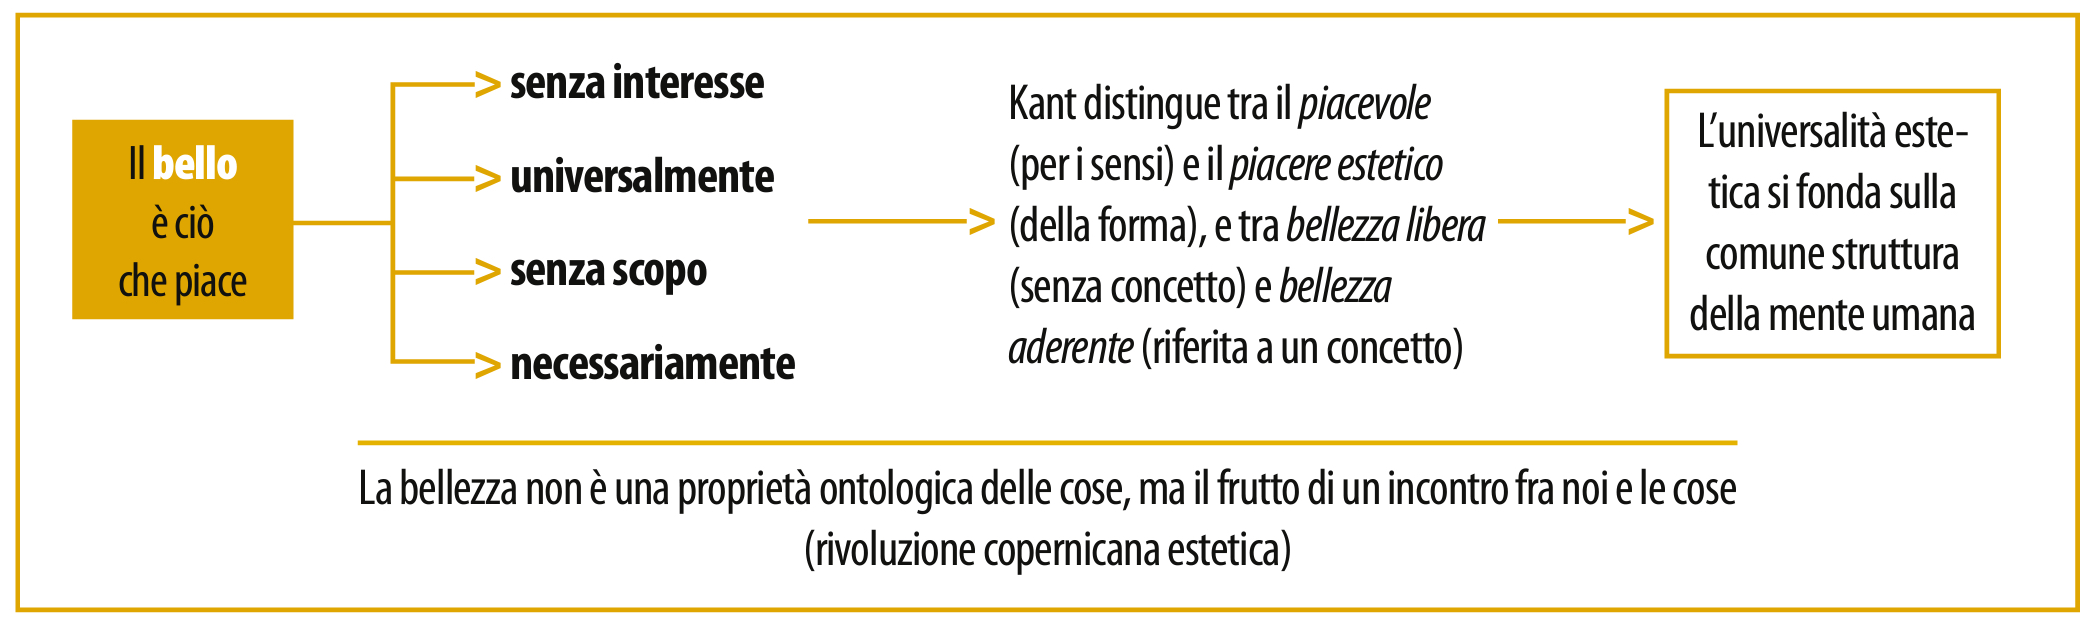
\includegraphics[width=12cm]{1}
\end{center}

\section{Sublime}

Ciò che è \textbf{sublime} per Kant mette in moto una dinamica di attrazione, repulsione, paura e senso di piccolezza, che poi viene in qualche modo superato.

\citazione{Sentimento di dilettoso orrore che l'uomo nella sua piccolezza prova e di fronte a ciò che non può controllare ma che può contemplare senza correre pericolo}

Il sublime viene diviso in due categorie
\begin{itemize}
\item \textbf{sublime matematico}, che nasce in presenza di qualcosa di smisuratamente grande, che provoca in noi uno stato d'animo ambivalente: da un lato proviamo dispiacere, perché la nostra immaginazione non riesce ad abbracciarne le incommensurabili grandezze;  dall’altro proviamo piacere,  perché la nostra ragione è portata da tali spettacoli a elevarsi all’idea dell’infinito,  in rapporto a cui le stesse immensità del creato appaiono piccole;
\item \textbf{sublime dinamico}, che nasce in presenza di poderose forze naturali; avvertiamo la nostra  piccolezza  materiale  e la nostra  impotenza nei confronti della  natura; in seguito, proviamo un vivo sentimento di piacere per la nostra  grandezza spirituale,  dovuta alla nostra realtà di esseri umani pensanti.
\end{itemize}

In entrambe le forme di sublime è necessaria la consapevolezza della nostra grandezza spirituale, perché senza di questa si riduce semplicemente a \textbf{terrore}. Viene visto solo da chi è in grado di vederlo.
Il bello è un equilibrio tra intelletto ed immaginazione, questo ci porta calma e serenità.
Il sublime invece fa leva sull’informe.

\section{Il bello nell'arte}

Il bello estetico ed il bello di natura possono essere affini.

\begin{itemize}
\item La natura è bella quando ha l’apparenza dell’arte
\item L’arte è bella quando ha l’apparenza e la spontaneità della natura
\end{itemize}

\subsection{Arte estetica}

Si divide in
\begin{itemize}
\item \textbf{Arte piacevole}: indirizzata ad uno scopo secondario come rallegrare ed intrattenere.
\item \textbf{Arte bella}: fatta per essere contemplata, non ha uno scopo esterno, non è fatta per procurare piacere, sarà lo spettatore che vedendola proverà un piacere disinteressato. Nasce dal genio, intermediario tra arte e natura, l’arte vera e propria nasce solo dalla spontaneità del genio.
\end{itemize}

Per essere compreso non serve il geno, basta solo avere buon gusto.

Il \emph{genio} è una capacità donata senza alcuno schema dalla natura ad alcuni esseri umani, con capacità superiori agli altri. Nato per non essere sprecato, per esprimere a pieno l’essenza dell’uomo. È il talento che dà la regola all’arte. È una predisposizione dell’anima che lo rende intermediario tra arte e natura. Fa arte dalla natura e fa della natura arte. È impossibile dimostrare scientificamente questa capacità. Se nella scienza operano degli ingegni, nell’arte operano dei geni.

\section{Giudizio teleologico}

Davanti alla vista della natura, si tende a pensare che ci sia stata una forza che abbia creato tutto senza alcun altro fine che per darlo come è. L’uomo tende a pensare che il modo sia stato creato su misura per lui.
Questo giudizio non è scientifico ma è appunto teleologico perché si basa su uno scopo primo che si trova oltre alle nostre conoscenze. Mi spinge comunque verso la ricerca, nonostante non sia scientifico.

\subsection{Antinomia del giudizio teleologico}

Deriva dal considerare i principi del giudizio riflettente, come principi costituivi degli oggetti. Giudizio scientifico e teleologico non sono in concorrenza tra di loro, e non creano antinomia se considerate nei loro giusti limiti ed ambiti.


\part{I critici immediati di Kant}

\chapter{Introduzione}

I "critici" o "seguaci immediati di Kant" criticano tutti i dualismi della filosofia kantiana, ed in particolar modo il dualismo di tutti i dualismi, ovvero \textit{la distinzione tra fenomeno e noumeno}. Partendo dalla presunta "contraddizione" di base di Kant, il quale avrebbe dichiarato estistente e al tempo stesso inconoscibile la \textbf{cosa in sé}, essi prendono di mira soprattutto il \emph{\textbf{concetto di nuomeno}}, giudicandolo filosoficamente inammissibile.

La \emph{prima critica} è la seguente: secondo Kant ogni realtà di cui siamo consapevoli esiste come rappresentazione della coscienza, la quale funge, a sua volta, da condizione indispensabile del conoscere. Ma se l'oggetto risulta concepibile solo in relazione a un soggetto che lo rappresenta, come può venir ammessa l'esistenza di una cosa in sé, ossia di una realtà non pensata e non pensabile, non rappresentata e non rappresentabile?
Evidentemente la cosa in sé, da un tale punto di vista, non può configurarsi che come un concetto impossibile.

Questa interpretazione vede nel pensiero di Kant
\begin{itemize}
\item una riduzione del fenomeno a semplice "rappresentazione"
\item una riduzione della cosa in sé come semplice "oggetto di rappresentazione"
\end{itemize}

In verità Kant identifica il fenomeno con "l'oggetto della rappresentazione", facendo intendere che il fenomeno non è una rappresentazione o un'idea, che giace dentro la coscienza, ma un oggetto reale, anche se viene appreso tramite il corredo mentale delle forme a priori.

Un \emph{altro appunto} mosso a Kant consiste nella tesi secondo la quale il filosofo, asserendo che la cosa in sé è causa delle nostre sensazioni, si sarebbe contraddetto, applicando anche al noumeno il concetto di causa ed effetto, valido soltanto per il fenomeno. In realtà, invece, il noumeno, per noi, non costituisce una realtà a cui applicare delle categorie, ma un semplice \textit{memento} critico, un "promemoria", che ci ricorda costantemente che l'oggetto ci è dato attraverso una rete di forme a priori.

\chapter{L'Io infinito di Fichte}

Kant aveva riconosciuto nell'io penso il principio supremo di tutta la conoscenza; questo però supponeva come data l'esistenza; era quindi attività limitata dall'intuizione sensibile.

Fichte idealizza l'\emph{Io come unico principio}, non solo formale, ma anche materiale, del conoscere.
L'Io si pone da se. Infatti la sua caratteristica consiste nell'\textbf{autocreazione}. Tale autocreazione coincide con l'intuizione intellettuale che l'Io ha di se stesso, in quanto attività in virtù della quale conoscere qualcosa si identifica con il produrre questo qualcosa. L'essere dell'Io appare come il frutto della sua stessa azione e il risultato della sua stessa libertà.

Tale prerogativa dell'Io viene denominata da Fichte \emph{Tathandlung}. L'Io è, nello stesso tempo, \textbf{attività agente} (\textit{Tat}) e \textbf{prodotto dell'azione} stessa (\textit{Handlung}).

Si noti come Fichte, con questo basilare principio, non faccia altro che portare alla massima espressione metafisica la visione rinascimentale emoderna dell'uomo come essere che costruisce o inventa se medesimo tramite la propria libertà.

I \emph{tre principi} su cui si basa la dottrina di Fichte, denominata \textit{Dottrina della scienza}, sono:
\begin{enumerate}
\item L'Io pone se stesso; il concetto di io in generale si identifica con quello di un'attività autocreatrice e infinita
\item L'Io pone il non-io; l'Io non solo pone se stesso, ma oppone anche a se stesso qualcosa che non è. Tale non-io è tuttavia posto dall'Io, ed è quindi nell'Io.
\item L'Io, avendo posto il non-io, si trova limitato da esso, Con il terzo principio perveniamo alla situazione concreta del mondo, in cui abbiamo una molteplicità di io finiti che hanno di fronte a sé una molteplicità di oggetti a loro volta finiti.
\end{enumerate}

\begin{center}

\includegraphics[width=12cm]{2}
\end{center}

Questi tre principi stabiliscono
\begin{itemize}
\item l'esistenza di un \textbf{Io infinito}, attività assolutamente libera e creatrice;
\item l'esistenza di un \textbf{io finito}, cioè di un soggetto empirico
\item la realtà di un non-io, cioè dell\textbf{oggetto}.
\end{itemize}

I tre principi non vanno interpretati in modo cronologico, bensì logico. Fichte non intende dire che esista prima l'Io infinito, poi l'Io che pone il non-io e infine l'io finito, ma semplicemente che esiste un Io che, per poter essere tale, deve presupporre di fronte a sé il non-io, trovandosi in tal modo a esistere concretamente sotto forma di io finito.
Fichte ha voluto mettere bene in luce come la natura non sia una realtà autonoma, che precede lo spirito, ma qualcosa che esiste soltanto come momento dialettico della vita dell'Io, e quindi \textit{per} l'Io e \textit{nell}'Io.

L'Io di Fichte risulta finito e infinito allo stesso tempo.

L'Io infinito non è qualcosa di diverso dall'insieme degli io finiti, esattamente come l'umanità non è qualcosa di diverso dai vari individui che la compongono.

L'Io infinito, più che la sostanza o la radice metafisica degli io finiti, è la loro meta ideale. L'infinito, per l'uomo, anziché consistere in un'essenza già data, è, in fondo, un dover essere e una missione. L'uomo è uno sforzo infinito verso la libertà, ovvero una lotta inesauribile contro il limite: il compito proprio dell'uomo è l'umanizzazione del mondo.

Ovviamente questo compito si staglia sull'orizzonte di una missione mai conclusa, poiché se l'Io, la cui essenza è lo sforzo, riuscisse davvero a superare tutti i suoi ostacoli, cesserebbe di esistere, e al movimento della vita, che è lotta e opposizione, subentrerebbe la stasi della morte.

Al posto del concetto statico di perfezione, tipico della filosofia classica, con Fichte subentra quindi un concetto dinamico, che pone la perfezione nello sforzo indefinito di autoperfezionamento.


\part{Hegel}

\chapter{Introduzione}

\textbf{Georg Wilhelm Friedrich Hegel} nacque il 27 agosto 1770 a Stoccarda. L’idealismo è la filosofia del romanticismo. Hegel è un filosofo estremamente complesso. La prima grande opera Hegel è la \textit{Fenomenologia dello spirito}. Dopo la sua morte i suoi studenti raccolsero, ordinarono e pubblicarono i suoi corsi di Berlino.

Gli scritti del periodo giovanile mostrano un prevalente interesse religioso-politico. Inizialmente l'argomento che proprio domina sul suo pensiero è un argomento teologico. D'altra parte con l’idealismo, venendo meno il limite tra fenomeno e noumeno la filosofia si configura come una filosofia dell'assoluto.

L’assoluto può essere interpretato in vari modi, ma sicuramente l'interpretazione teologica, cioè vedere l'assoluto come Dio, è più facile e istintiva. Però il suo interesse teologico si lega alla politica.
Chi è convinto che il tema della rigenerazione religiosa e quindi morale dell'uomo coincida con la rigenerazione politica? Platone

Platone aveva cominciato a esprimere le sue teorie filosofiche proprio quando aveva cominciato a pensare che la sua società fosse malata, in cui la politica non era più pura come nell’età precedente, e soprattutto perché i politici del suo tempo avevano ucciso Socrate, l’uomo più giusto di tutta la società. Per Platone tutto questo è inaccettabile. Platone era partito con l’idea che, migliorare la cultura tramite la filosofia sarebbe servito a migliorare la società e quindi la politica.

Anche Hegel pensa qualcosa di simile. Lui pensa che si debba cambiare la società: siamo nella fase che va dalla Rivoluzione Francese al Congresso di Vienna; sono anni molto ricchi politicamente, c'è una società in fibrillazione, che vuole essere cambiata. Egli è convinto che non si possa realizzare alcuna autentica rivoluzione politica se non basandola su una rivoluzione culturale, ovvero una rigenerazione della persona nella sua vita interiore e del popolo nella sua cultura. Hegel è convinto che il valore della filosofia permetta una rigenerazione culturale.

Lui pensa che i popoli, aspirando alla libertà e ad una vita migliore (avendone il diritto di farlo), normalmente combattono la vecchia struttura sociale. Una società basata sulla stratificazione sociale doveva cambiare. Pensa che si debba dare spazio a questo desiderio di liberà dei popoli, vuole quindi usare cultura e filosofia per liberare i popoli. Si doveva lavorare, attraverso la cultura e quindi la filosofia, per alimentare il desiderio di liberà dei popoli. L'idea di fondo è che l'aspirazione dei popoli a una vita migliore e alla liberà deve tradursi in realtà vivente attraverso la realizzazione di progetti di riforma che spazzino via il vecchio impianto sociale.

Hegel è dunque convinto che la rivoluzione nelle istituzioni possa avvenire solo come conseguenza esteriore di una maturazione avvenuta all'interno della coscienza del popolo.

Egli chiarisce anche il nesso tra religione e politica. Perché giungano i "tempi migliori", occorre una nuova forma di religione, che permetta a ciascuno dei cittadini di partecipare con la propria vita interiore alla vita dello spirito di Dio, che si incarna nella storia non attraverso leggi e precetti morali, ma attraverso la stessa vita degli uomini. Potrà nascere un ordine politico egualitario quando i cittadini avranno imparato a vivere la religione come comunanza dei cuori, quando ciascuno di essi avrà imparato a riconoscere nella vita interiore il riflesso dell'unica vita di Dio.

Tutto l'impianto filosofico di Hegel è basato sul desiderio di dare una forma politica della sua filosofia. La concezione che Hegel maturerà di stato, di società civile, di leggi, è una delle più belle e più ricche della storia della filosofia, degna di essere ancora oggi tra quelle più considerate.

\chapter{Capisaldi del sistema}

Questi tre capisaldi non sono tre argomenti che Hegel ha trattato in questi termini. Hegel ha esposto il suo sistema, e per ragione di comodità gli studiosi hanno estratto queste tre linee.
\begin{enumerate}
\item Risoluzione del finito nell'infinito
\item Identità fra realtà e ragione, che si esprime nel celebre aforisma
\citazione{ciò che è razionale è reale ciò che è reale è razionale}
\item La funzione della filosofia, che è una funzione giustificatrice
\end{enumerate}

\section{Primo caposaldo: risoluzione del finito nell'infinito}

In questo caposaldo si dice che la realtà deve essere considerata come un organismo unitario, che è l'\textbf{assoluto} (l'Io per Fichte).

Per Hegel la realtà non è un insieme di sostanze autonome, ma un organismo unitario di cui tutto ciò che esiste è parte o manifestazione. Tale organismo, non avendo nulla al di fuori di sé, coincide con l'\textbf{Assoluto} e con l'\textbf{infinito}, mentre i vari enti del mondo, essendo manifestazioni di esso, coincidono con il finito.
Tutto ciò che esiste è l'assoluto, e tutto ciò che noi vediamo, anche quello che è finito, è una manifestazione di questo assoluto.

Non abbiamo quindi il finito e l'infinito, ma abbiamo un'unica grande realtà infinita in cui esiste il finito, ovvero i vari enti del mondo, che sono manifestazioni dell'infinito.
Il finito non esiste come entità a sé, ma esiste come espressione parziale dell'infinito.

Come la parte non può esistere se non in connessione con il tutto, in rapporto al quale soltanto ha vita e senso, così il finito esiste unicamente nell'infinito e in virtù dell'infinito.

Si giunge ad un \textbf{monismo panteistico}, cioè come una teoria che vede nel mondo la manifestazione o la realizzazione di Dio. Questo assomiglia alla visione di Spinoza, che vide per la prima volta coincidenti nella sostanza Natura e Dio.

Mentre per Spinoza l'Assoluto è una sostanza statica che coincide con la natura, per Hegel invece si identifica con un soggetto spirituale in divenire, di cui tutto ciò che esiste è momento o tappa di un processo di realizzazione.
Spinosa non aveva parlato di un’attività dinamica all’interno della sostanza stessa, era vista come statica. L’assoluto, la sostanza, erano quindi per lui formati da corpo e spirito insieme.

Per gli idealisti all’interno di questo insieme, vige un processo di autoproduzione e crescita continua basata sulla dialettica come movimento continuo. Dire che la realtà non è sostanza ma soggetto, significa dire, secondo Hegel, che essa non è qualcosa di immutabile e di già dato, ma un processo di auto-produzione che soltanto alla fine, cioè con l'uomo giunge a rivelarsi per quello che è veramente.

Questo si rispecchia in una chiave panteistica, vedere Dio nella natura e la natura in Dio.

\begin{center}
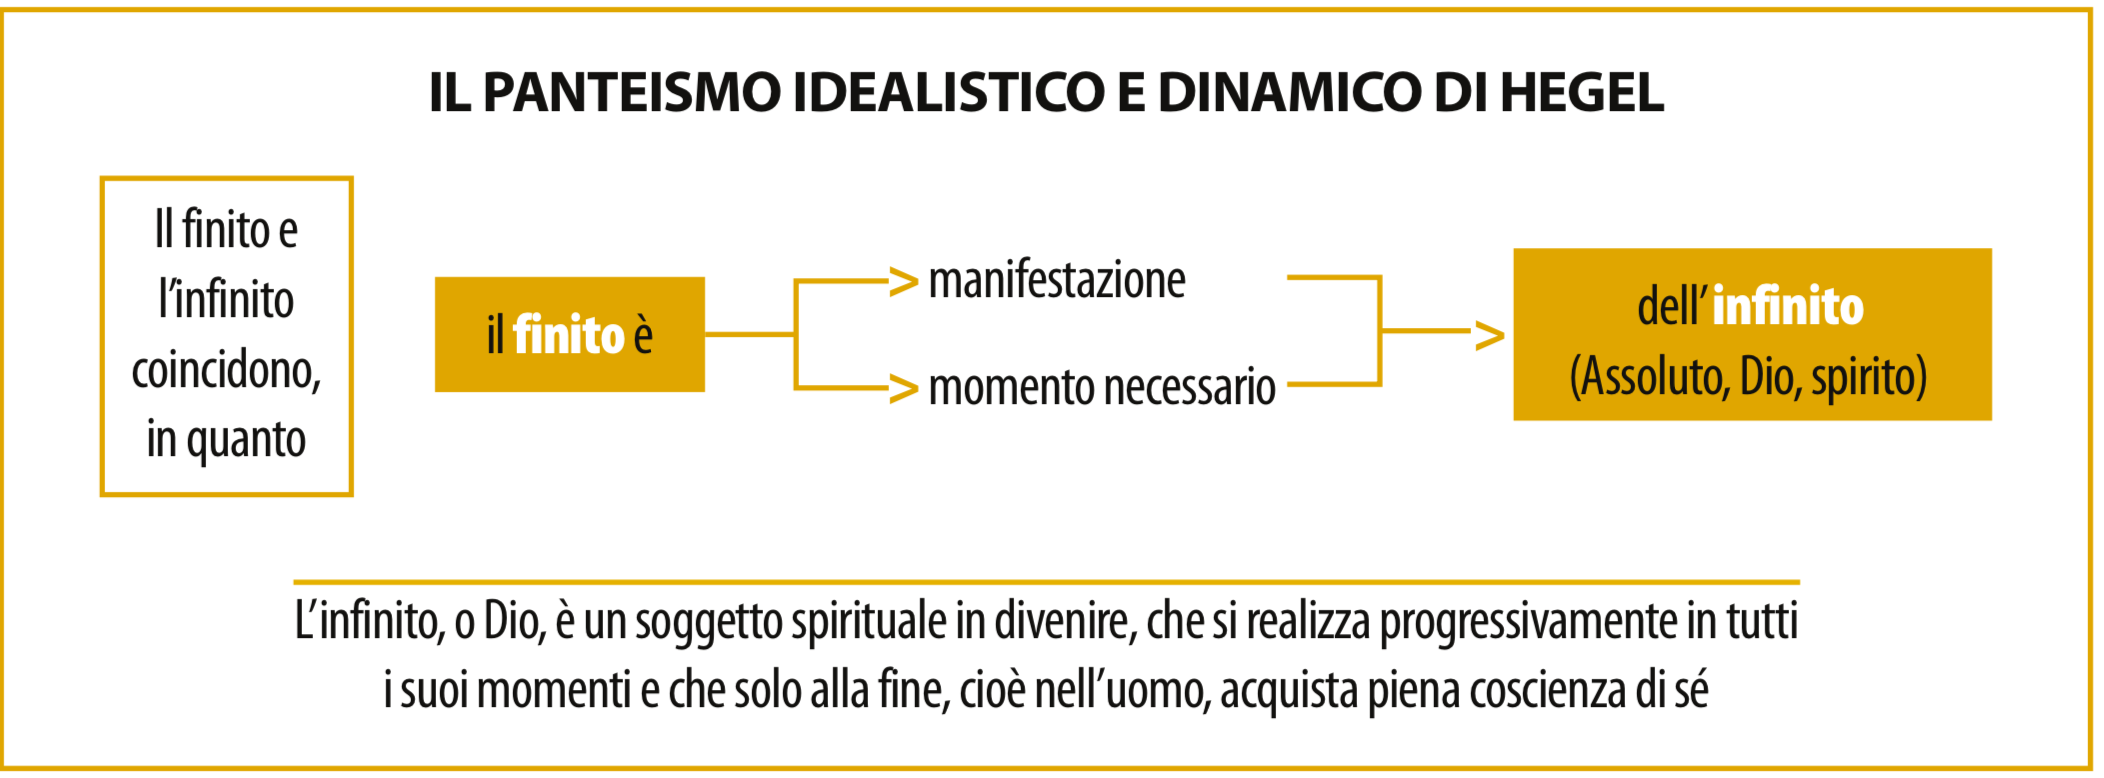
\includegraphics[width=12cm]{3}
\end{center}
% ![image\textit{2021-01-11}21-15-53](/assets/image\textit{2021-01-11}21-15-53.png)

\section{Secondo caposaldo: Realtà e Ragione}

La relazione che c'è tra questi due elementi è espressa dall'aforisma

        Ciò che è razionale è reale; e ciò che è reale è razionale

Nonostante la similitudine con il primo caposaldo, aggiunge nel finito un significato e una ragione. La realtà non è qualcosa di accidentale e casuale, ma è il risultato di un processo razionale che è guidato dalla Ragione stessa.

La \emph{Ragione} è il progetto razionale sulla base del quale la realtà si sviluppa.

Volendo interpretare questo in chiave teologica, si potrebbe dire che c'è una divinità che ha determinato ciò che è il modo, che lo governa, e che ha nei confronti di questo mondo reale un \emph{progetto}. Questo progetto non punta al benessere.

La Realtà quindi non è caotica, ma è il dispiegarsi di una \emph{struttura razionale}. Noi uomini, però non siamo in grado di comprendere questa struttura, né tantomeno le ragioni.

Ciò che è la realtà è così perché \textbf{deve essere così}. Il mondo non potrebbe essere diverso da così. Le manifestazioni sono \emph{\textit{momenti necessari}}

\section{Terzo caposaldo: funzione della filosofia}

La funzione della filosofia non è di guidare il mondo, ma di aiutare l'uomo a \emph{comprendere le strutture razionali} che stanno dietro alla ragione. La funzionalità che sta dietro al grande progetto della Ragione può essere indagata, attraverso la ragione umana, con la filosofia.

La filosofia deve \emph{rinunciare alla pretesa di guidare il mondo}, perché il mondo va da sé, secondo un progetto necessario.

\subsection{Giustificazionismo Hegeliano}

Hegel tiene a specificare che egli per realtà non intenda ogni singolo aspetto dell'esistente: per lui un'esistenza accidentale non merita il nome di realtà.

Altre accuse vedono Hegel additato come conservatore, in quanto, se la realtà deve necessariamente essere com'è non vi è alcun adito a rivoluzioni.
L'errore, però, risiede nel fatto che la realtà, per quanto razionale, non deve necessariamente essere la migliore possibile, ma solo uno stadio, necessario, atto a raggiungere un fine ultimo, non conoscibile dall'uomo.

Ad ogni modo, le evidenze sembrano suggerire che in Hegel vi sia un sostanziale giustificazionismo della realtà

I critici successivi di Hegel si dividono di \textbf{destra} e \textbf{sinistra hegeliana}.

La \emph{destra hegeliana} ha caratteri più conservatore

La \emph{sinistra hegeliana} rielabora il pensiero del filosofo in chiave rivoluzionaria, soprattutto negli ambiti religiosi e sociali: esempi sono Marx e Foierback.

\chapter{Le partizioni della filosofia}

Hegel ritiene che il farsi dinamico dell'Assoluto passi attraverso i tre momenti dell'idea
\begin{enumerate}
\item L'idea in sé: \textbf{tesi}. Si tratta dell'idea considerata in se stessa, a prescindere dalla sua attuazione reale. Hegel la paragona all'ossatura logico-razionale della realtà
\item L'idea fuori di se: \textbf{antitesi}. È la natura, ovvero l'alienazione dell'idea nelle realtà del mondo
\item L'idea che ritorna in sé: \textbf{sintesi}. È lo spirito, ovvero l'idea che dopo essersi fatta natura, torna nell'uomo.
\end{enumerate}

Ovviamente questa triade non va intesa in senso cronologico, ma in senso ideale.

Kant associa a questi tre momenti strutturali dell'Assoluto le tre sezioni in cui si divide il sapere filosofico
\begin{enumerate}
\item \textbf{Logica}, ovvero la scienza dell'idea
\item La \textbf{filosofia della natura}, ovvero lo studio dell'idea fuori di se
\item La \textbf{filosofia dello spirito}, ovvero lo studio dell'idea che ritorna in sé.
\end{enumerate}

% ![Schermata 2021-02-01 alle 22.49.43](/assets/Schermata%202021-02-01%20alle%2022.49.43.png)
\begin{center}
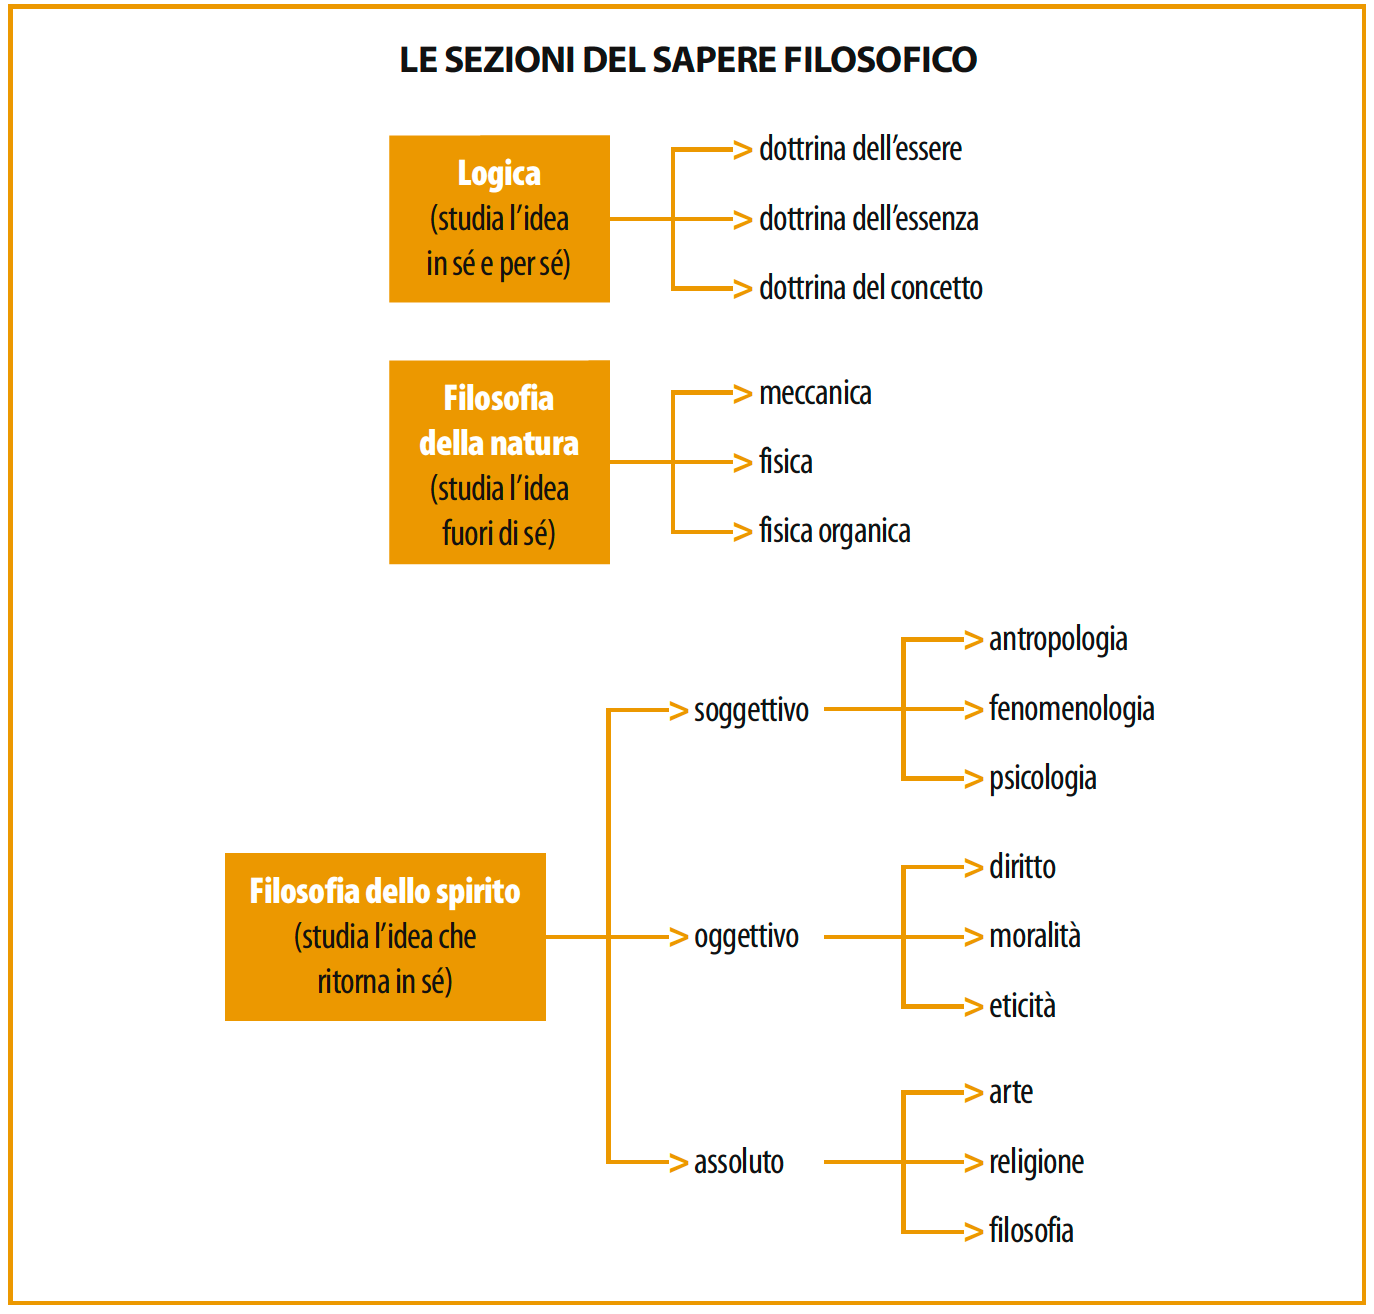
\includegraphics[width=12cm]{4}
\end{center}

\chapter{Dialettica}

L'assoluto, per Hegel, è fondamentalmente divenire. La \emph{\textbf{dialettica}} è sia la legge ontologica di sviluppo della realtà che la legge logica di comprensione della realtà. Hegel distingue tre momenti del pensiero.

\section{Momento astratto (o intellettuale)}

Questo momento consiste nel concepire l'esistente sotto forma di una molteplicità di determinazioni statiche e separate le une dalle altre; (principio di identità).
 
\section{Momento dialettico (o negativo-razionale)}

Questo momento consiste nel mettere in rapporto le varie determinazioni con le determinazioni opposte, andando oltre il principio di identità.

\section{Momento speculativo (o positivo-razionale)}

Il terzo momento consiste nel cogliere l'unità delle determinazioni opposte, comprendendo che sono aspetti di una realtà che li sintetizza entrambi.

\medskip\hrule\medskip

Globalmente parlando, la dialettica consiste quindi nell'\textbf{affermazione} di un concetto che funge da tesi; nella negazione di questo concetto, che funge da antitesi; nell'\textbf{unificazione} delle precedenti affermazione e negazione in una sintesi positiva comprensiva di entrambe.

% ![Schermata 2021-02-01 alle 23.07.42](/assets/Schermata%202021-02-01%20alle%2023.07.42.png)
\begin{center}
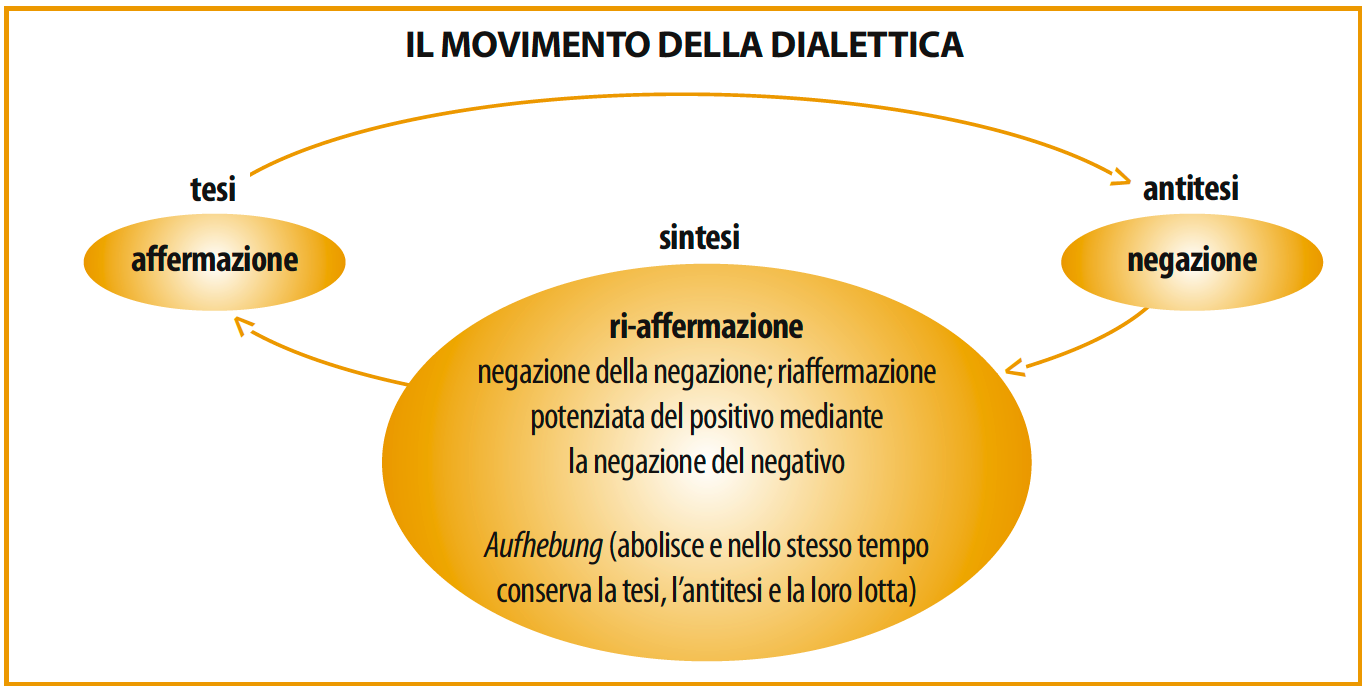
\includegraphics[width=12cm]{5}
\end{center}

La sintesi, quindi, si configura come una riaffermazione potenziata della tesi. Il termine tecnico con cui Hegel si riferisce a ciò è \textbf{Aufhebung}, che esprime l'idea di un superamento (quello dell'antitesi), che è sia un togliere che un conservare.

La Dialettica non fa che illustrare il principio fondamentale della filosofia hegeliana: la risoluzione del finito dell'infinito: ogni realtà non può esistere in sé stessa, ma solo in un contesto di rapporti; il finito, per esistere, deve opporsi all'infinito.

La Dialettica ha un significato ottimistico, perché unifica il molteplice e unisce le opposizioni.

Hegel pensa che il processo dialettico sia chiuso, ovvero che, a furia di contrapporre tesi e antitesi, si raggiunga una sintesi "finale".

Tutti i filosofi successivi, che si rifaranno all'hegelismo, criticheranno questa idea, recuperando l'idea di un processo aperto.

\chapter{\textit{Fenomenologia dello spirito}}

È un’opera all’interno della \textit{Filosofia dello spirito}. Sulla parte della \emph{fenomenologia} Hegel apre una parentesi.
La "fenomenologia" di per sé è la scienza di ciò che appare; pertanto, la "fenomenologia dello spirito" è l'apparire dello spirito a sé stesso.

La fenomenologia dello spirito è la storia romanzata della \emph{coscienza umana}, definita coscienza infinita: è la coscienza dell’uomo che, attraverso un percorso complicato arriva a riconoscere se stessa come parte del tutto e uscire dall’individualità.
Tutto ciò è raccontato in figure: sono tappe storico-ideali che rappresentano dei momenti importanti della storia dell’uomo.

Con \textit{uomo} si intende sia il genere umano, che come singolo individuo: Hegel è convinto che la \emph{storia dell’umanità} rappresenti in grande ciò che in piccolo è la \emph{storia di ognuno di noi}.

Hegel studia la risoluzione del finito nell'infinito, in due modi diversi:
\begin{itemize}
\item in senso \textbf{diacronico}, ovvero il lungo viaggio che lo spirito compie per comprendere se stesso quale Assoluto (trattato appunto nella \textit{Fenomenologia dello spirito})
\item in senso \textbf{sincronico}, ovvero l'eterna coesistenza nel reale dei tre momenti dell'Assoluto (trattato nell'\textit{Enciclopedia delle scienze filosofiche in compendio}).
\end{itemize}

L'intera opera si può riassumere nella figura della \emph{\textbf{coscienza infelice}} che non sa di essere tutta la realtà, e pertanto si ritrova scissa in opposizioni e conflitti dai quali è dilaniata, e che risolverà solo arrivando alla coscienza di essere tutto.

L’opera si articola in tre parti:
\begin{itemize}
\item Coscienza
\item Autocoscienza
\item Ragione
\end{itemize}

\section{Coscienza}

Nella parte della \emph{coscienza} l’attenzione è sul mondo esterno. La coscienza nasce nel soggetto quando questo acquisisce la consapevolezza del mondo esterno: si crea una relazione tra il soggetto e l’oggetto.
Il punto di partenza è la certezza sensibile.
Il bambino inizia a conoscere l’esterno: allo stesso modo i primi filosofi si concentrano sull’\textit{Arché}, sul mondo esterno; solo con Socrate si concentreranno sull’uomo.
La conoscenza del mondo, in questa fase, ha forti riferimenti Kantiani.

\section{Autocoscienza}

L’\emph{autocoscienza} è il momento che fa sì che l’attenzione si sposti dall’esterno all’interno: dall’oggetto al soggetto. È la parte più lunga, sia della vita che della storia dell’umanità.
Questo passaggio dura molto, è complesso, e da un punto di vista storico Hegel identifica la fine di questa fase con l’Umanesimo e il Rinascimento.
Non siamo più sul piano gnoseologico

\subsection{Signoria e servitù}

Hegel identifica la figura di \emph{\textbf{signoria e servitù}}: è la relazione tra servo e signore, non solo tipica del mondo antico, ma presente tutt’oggi.
Vi è un servo e un signore: nella storia questa figura è importantissima.
Il servo è colui che si abitua al sacrificio, alla fatica: sviluppa una consapevolezza di sé che il signore spesso non ha.

L'uomo è autocoscienza solo se riesce a farsi \emph{riconoscere} da un'altra autocoscienza. Inizialmente Hegel era convinto che il riconoscimento di sé avvenisse per mezzo dell’amore, ma all'amore manca la serietà, il dolore, la pazienza e il travaglio del negativo. In un secondo momento egli cambia idea: quello che fa veramente capire cosa sia la vita è il conflitto: si torna alla dialettica.

Il riconoscimento di sé che passa attraverso il \emph{conflitto} mi rende consapevole di quello che sono. Egli sviluppa l’idea che il conflitto sia, da un punto di vista pedagogico, più utile del conflitto positivo; ecco perché la scelta di una figura così contrastante.
Il conflitto non si conclude con la morte delle autocoscienze, ma con il subordinarsi dell'una all'altra nel rapporto servo-signore.

La dinamica del rapporto servo signore è destinata a a mettere a capo una paradossale \emph{inversione dei ruoli}. Infatti il signore, che inizialmente appariva indipendente, nella misura in cui si limita a godere passivamente del lavoro dei servi, finisce per dipendere da loro. Invece il servo, che inizialmente appariva dipendente, nella misura in cui padroneggia e trasforma le cose da cui il signore riceve il proprio sostentamento, finisce per rendersi indipendente, sviluppando il senso di sé.

Ci sono tre fasi in cui il servo sviluppa il senso di sé:
\begin{enumerate}
\item Paura della morte
\item Servizio
\item Lavoro
\end{enumerate}

\subsubsection{Paura della morte}

Il servo, dopo aver tremato dinnanzi alla possibilità della morte, con la conseguente perdita assoluta della propria essenza, ha potuto sperimentare il proprio essere come qualcosa di distinto o di indipendente da quel mondo di realtà e di certezze naturali che prima gli apparivano come qualcosa di fisso e con le quali si identificava.

\subsubsection{Servizio}

Nel servizio la coscienza si autodisciplina e impara a vincere, in tutti i singoli momenti, i propri istinti naturali.

\subsubsection{Lavoro}

Nel lavoro il servo rimanda il momento dell'utilizzo dell'oggetto che sta producendo; egli da luogo ad un'opera che ha una sua indipendenza; l'opera prodotta rappresenta l'autonomia del servo rispetto agli oggetti.
In tal modo, egli giunge ad intuirsi come essere indipendente.

\subsection{Stoicismo e scetticismo}

La storia è caratterizzata dalla ricerca dell'uomo di trovare conforto nella filosofia. Il filosofo, non essendo più rappresentato dalla politica, si chiude nella filosofia, alla ricerca della soluzione ai propri problemi.

Questo succede nell'epoca ellenistica, appunto con i movimenti filosofici di \textit{stoicismo} e \textit{scetticismo}; i cittadini, sentendosi sudditi, si allontanano dalla scena politica e si chiudono nella filosofia.

È il momento in cui l'autocoscienza si vuole liberare dal mondo esterno, decondizionandosi dalle cose, raggiungendo l'indipendenza.

Gli stoici ci provano, ma il tentativo non va a buon fine.

Lo scetticismo, ci prova con maggiore forza, in quanto gli scettici mettevano il mondo tra parentesi, ritenevano che non si potesse essere certi di nulla; cercavano una interiorità che si distaccasse dal mondo. Secondo Hegel però non si produce un vero distacco, in quanto gli scettici si auto-contraddicono (dicono che tutto sia falso, ma ritengono la loro filosofia vera).

\subsection{Ebraismo e cristianesimo}

La coscienza infelice, ovvero la protagonista della \textit{Fenomenologia dello spirito}, è quella che non sa di essere tutta la realtà e che perciò si trova scissa in differenze, opposizioni e conflitti dai quali è dilaniata.

In ambito religioso incontra si esprime in due figure consecutive: \textbf{Ebraismo} e \textbf{Cristianesimo}
\begin{itemize}
\item L'ebraismo parla di un Dio trascendente, padrone assoluto: possente, autoritario, come un padre o un padrone
Il fedele non si trova a suo agio, ma è in una situazione di dipendenza: è qualcosa di faticoso e di pauroso.
\item Il cristianesimo presenta un avvicinamento a Dio tramite Cristo: la religiosità porta ad un avvicinamento e ad un ritrovamento di sé stesso: non porta alla realizzazione, ma alla tristezza e al terrore.
\end{itemize}

Anche questa forma però è destinata al fallimento. Ad esempio nelle crociate la ricerca di Dio si conclude con la scoperta di un sepolcro vuoto.
Inoltre Cristo è sempre qualcosa di vuoto e separato della coscienza.
Perciò anche con il cristianesimo la coscienza continua a rimanere infelice.
Manifestazioni di questa infelicità cristiano-medioevale sono le sottofigure
Della \textit{devozione}, del \textit{fare} e della \textit{mortificazione di sé}.

La religiosità è il punto più basso dell'uomo: se continua da solo in questo percorso, non arriverà da nessuna parte, e sarà fallimentare. L'uomo a questo punto si ferma a ragionare: si ha il passaggio tra \textbf{autocoscienza a ragione}.
Storicamente questa fase si identifica con il rinascimento: si ha un distacco dal mondo esterno; l'uomo pone se stesso al centro del mondo, con la rivoluzione scientifica

\section{Ragione}

L'autocoscienza come soggetto assoluto ha assunto in sé ogni realtà ed è diventata \textbf{Ragione}. Ora sa che la realtà non è diversa da sé. Deve però trovare una giustificazione: i momenti di questo percorso sono:
\begin{itemize}
\item la ragione osservativa
\item la ragione attiva
\item l'individualità in sé e per sé
\end{itemize}

\subsection{Ragione osservativa}

Nella ragione osservativa la coscienza si rivolge al mondo della natura, credendo di trovare l'essenza delle cose. In realtà cerca sé stessa.
L'osservazione si approfondisce con la ricerca della legge e con l'esperimento, con il metodo scientifico, per arrivare allo studio della coscienza stessa con la psicologia.

In questa ricerca esasperata di se stessa, la ragione sperimenta la propria crisi, riconoscendosi come qualcosa di distinto dal mondo.

\subsection{Ragione attiva}

Nella ragione attiva è giunta a compimento la consapevolezza che l'unità di io e mondo non è qualcosa di già dato, ma deve venire realizzata. Questo progetto, se perseguito individualmente, cioè come lo sforzo dell'iniziativa della singola coscienza, è destinato a fallire.

\subsection{Individualità in sé e per sé}

Nell'individualità in sé e per sé Hegel dimostra che l'individualità, pur potendo raggiungere la propria realizzazione, rimane astratta ed inadeguata.
In sintesi Hegel ci dice che se ci si pone dal punto di vista dell'individuo si è inevitabilmente condannati a non raggiungere mai l'universalità

L'\textbf{universalità} si trova solo nella fase dello spirito, nelle istituzioni storico-politiche di un popolo e soprattutto nello Stato.
Anche le leggi etiche più indubitabili sono astrazioni se manca lo stato a darne il contenuto. La ragione reale non è quella dell'individuo, ma quella dello spirito o dello stato.

\chapter{Filosofia dello spirito}

È la conoscenza più alta e difficile, in quanto è lo studio dell'idea che, dopo essersi estraniata da sé, sparisce come oggettività, esteriorità e spazialità (natura) per farsi soggettività e libertà.

Lo sviluppo dello Spirito avviene attraverso tre momenti:
\begin{itemize}
\item Spirito Soggettivo (individuale)
\item Spirito Oggettivo (sovraindividuale o sociale)
\item Spirito Assoluto (che conosce se stesso nelle forme dell'arte, della religione e della filosofia)
\end{itemize}

Lo spirito procede per gradi: ciascuno di essi è compreso e risolto nel grado superiore ed è già presente nel grado inferiore.

\section{Spirito soggettivo}

È lo spirito individuale considerato nel suo progressivo emergere dalla natura. Va verso forme di vita psichica più complesse.

Lo spirito soggettivo ha una consapevolezza elevata, con un percorso da fare, che porta da una vita psichica semplice a complessa. Si divide in tre parti:
\begin{itemize}
\item L'\textit{}antropologia\textit{} studia lo spirito come anima che si identifica con una fare aurorale della vita cosciente: è il dormiveglia dello spirito.
\begin{itemize}
  \item l'infanzia (tesi) è il momento in cui l'individuo è in armonia conn il mondo esterno
  \item la giovinezza (antitesi) è il momento del contrasto con il mondo
  \item la maturità (sintesi) è il momento della riconciliazione con il mondo
  \end{itemize}
\item Con la \textbf{fenomenologia} si ha la tripartizione già vista.
\item La \textit{}psicologia\textit{}: studia lo spirito in senso stretto, cioè nelle sue manifestazioni universali, e passa attraverso il conoscere, l'agire pratico ed il volere libero.
\end{itemize}

Non sono una triade dialettica, ma tre diversi sviluppi.

\section{Spirito oggettivo}

La volontà di libertà, che si è manifestata nella fase finale precedente, si esprime nello spirito oggettivo, in cui lo spirito si manifesta in situazioni sociali concrete, ovvero nelle determinazioni sovraindividuali che costituiscono il diritto.

I momenti dello spirito oggettivo sono tre:
\begin{itemize}
\item diritto astratto
\item moralità
\item eticità
\end{itemize}

Lo spirito oggettivo porta in sé le conquiste fatte precedentemente. Si ha la consapevolezza del soggetto con l'oggetto.
Servono le forme istituzionali per imparare a stare con gli altri; sono determinazioni sovraindividuali del diritto.

\subsection{Diritto astratto}

CIl volere libero si manifesta nel volere del singolo individuo, come persona fornita di capacità giuridiche. Il diritto astratto riguarda l'esistenza esterna della libertà delle persone. Queste trovano la loro prima realizzazione in una cosa esterna attraverso il possesso delle cose (proprietà): è insito nell'uomo: l'uomo tende a dare dei confini, con la proprietà.

\begin{itemize}
\item Il contratto è l'elemento attraverso il quale gli altri riconoscono la proprietà di qualcuno. È il punto di partenza, la tesi.
\item L'antitesi è il torto (che nei casi più gravi diventa delitto).
\item La sintesi è la pena, che deve avere valore rieducativo, non vendicativo. Il carcere migliora: una persona che è passata attraverso le tre fasi di questa triade dialettica è migliore di qualcuno che non abbia mai sbagliato.
\end{itemize}

La proprietà è il punto di partenza: è uno statuto giuridico attraverso cui il soggetto realizza sé stesso in una cosa esterna.

Quando il bambino comincia a volersi affermare con altri bambini, inizia ad appropriarsi di un oggetto. Il possesso indica una forza, una presenza, da cui si sviluppa la relazione con gli altri.

La proprietà è sancita di fronte agli altri da un contratto. Nella società moderna si fa un \textbf{contratto} (tesi). L'antitesi del contratto è il \textbf{torto}, che nella sua forma più grave è \textit{delitto}.
La riabilitazione che avviene nel terzo momento della pena è la sintesi.

La pena deve essere rieducativa, e deve essere riconosciuta interiormente dal colpevole.

\subsection{Moralità}

È l'intenzione positiva che l'uomo ha di compiere delle azioni che lo portino verso il bene.

Ogni azione sgorga da un proponimento, il cui fine è il \textit{benessere}: non momentaneo, ma un progetto, anche a lunga scadenza.
Quando il benessere si solleva oltre la mia sfera soggettiva, ci si eleva alla moralità.

Il \textbf{bene in sé per sé} è qualcosa che deve essere ancora realizzato,  s è un progetto. La moralità ha un obiettivo: il bene mio e degli altri.
Nella moralità c'è una distinzione tra il soggetto che deve realizzare il bene e il bene che deve essere realizzato. Le due fasi sono disgiunti.

Nella morale ci può essere una contraddizione tra essere e dover essere.

\subsection{Eticità}

Non vi è più distanza tra il soggetto che deve realizzare il bene e il bene che deve essere realizzato. È la realizzazione della moralità.

Il bene viene attuato e diventa qualcosa di esistente.
La realizzazione del bene è data dalla sua concretizzazione nelle forme istituzionali; l'eticità è data dalla creazione delle forme istituzionali: queste forme sono
\begin{itemize}
\item la famiglia
\item la società civile
\item lo stato
\end{itemize}

\subsubsection{Famiglia}
La famiglia è il primo momento dell'incontro con la società. È basata su \textit{matrimonio}, \textit{patrimonio} ed \textit{educazione dei figli}.
È un gruppo chiuso, guidato dall'amore, e le persone si proteggono l'una con l'altra. È un nucleo positivo.

\subsubsection{Società Civile}
Le diverse famiglie si aprono al mondo. La società civile nasce nel momento in cui i nuclei chiusi delle famiglie entrano in contatto tra di loro. È un sistema potenzialmente conflittuale, diviso in tre momenti:
\begin{itemize}
\item sistema dei bisogni
\item amministrazione della giustizia
\item polizia e corporazioni
\end{itemize}

Con la formazione di nuovi nuclei il sistema unitario della famiglia si frantuma nel sistema atomistico e conflittuale della società civile. Questa si identifica con la sfera economico-sociale e giuridico-amministrativa del vivere insieme. È luogo di scontro ma anche di incontro.
\begin{itemize}
\item Il sistema dei bisogni:\\
	Nasce dal fatto che gli individui, dovendo soddisfare i loro bisogni mediante la produzione di ricchezza e divisione del lavoro, danno origine a diverse classi sociali:
	\begin{itemize}
		\item agricoltori (classe sostanziale), che ha come patrimonio i prodotti di un terreno che lavora
		\item artigiani (classe formale), che danno forma al prodotto naturale
		\item pubblici funzionari, che si occupano degli interessi di tutta la società.
	\end{itemize}
\item L'amministrazione della giustizia concerne la sfera delle leggi e si identifica con il diritto pubblico
\item La polizia e le corporazioni provvedono alla sicurezza sociale
Le corporazioni in particolare attuano una sorta di unità tra la volontà del singolo e la categoria lavorativa alla quale appartiene, e prefigurano il momento dell'universalità statale
\end{itemize}

L'idea di porre tra Stato ed individuo la società civile è ritenuta una delle maggiori intuizioni di Hegel. Questa verrà ampiamente ripresa ed utilizzata da successivi studiosi di problemi economici e sociali, e troverà in Marx un interprete originale.

\subsubsection{Stato}

Lo \textbf{Stato} rappresenta il momento culminante dell'eticità, ossia la riaffermazione dell'unità della famiglia (tesi) al di là della dispersione della società civile (antitesi).

Lo Stato è una sorta di famiglia in grande, nella quale un popolo esprime consapevolmente se stesso.
Lo Stato non implica la soppressione della società civile, che è un momento necessario, ma è concepito in modo etico, visto come \textit{incarnazione del bene comune} e della morale sociale.

Lo Stato non è visto come strumento volto a garantire la sicurezza e i diritti (come inteso in Kant), in quanto questo lo ridurrebbe a tutore dei vari particolarismi.
Lo Stato non è neppure quello del modello democratico, ovvero modello di sovranità popolare. La \textbf{sovranità} dello stato deriva da esso stesso in quanto lo stato ha in se stesso la propria ragione d'essere e non al di fuori.

Lo Stato non è dunque fondato sugli individui, ma sull'idea di Stato, ossia sul concetto di bene universale. Non sono gli individui a formare lo Stato, ma lo Stato a fondare gli individui, sia dal punti di vista storico-temporale, che dal punto di vista ideale. Si rifiuta quindi anche il modello contrattualisti, ovvero far dipendere la vita dello Stato da un contratto scaturente dalla volontà degli individui.
Per Hegel questo è un insulto all'autorità dello Stato. Hegel contesta anche il giusnaturalismo, ossia l'idea di diritti naturali esistenti prima ed oltre lo Stato. Lo Stato di Hegel non è dispotico, perché egli ritiene che debba agire attraverso le leggi e nella forma della legge. Questo in omaggio al principio che a governare non devono essere gli uomini, ma le leggi.

L'organizzazione dello Stato è data dalla Costituzione, che sgorga dalla vita di un popolo e non a tavolino.
Infatti, se si vuole imporre a priori una Costituzione ad un popolo, inevitabilmente si fallisce, anche se la costituzione è migliore di quella esistente.

Hegel identifica la Costituzione razionale con la monarchia costituzionale moderna, ossia un organo politico con poteri distinti, ma non divisi.
\begin{itemize}
\item \textbf{Potere legislativo}: consiste nel potere di stabilire e determinare l'universale e concerne le leggi come tali. L'assemblea di rappresentanza delle classi trova la sua espressione in una Camera Alta e una Camera Bassa.
Hegel, pur insistendo sull'importanza dei ceti mediatori, si dimostra diffidente verso l'agire politico di tali ceti perché questi possono tendere al loro interesse privato.
\item \textbf{Potere governativo}: comprende i poteri giudiziari e di polizia, già operanti all'interno della società civile, ed opera traducendo in atto, in riferimento a casi specifici, l'universalità delle leggi.
\item \textbf{Potere monarchico} (principesco): incarna l'unità dello Stato in una individualità reale. È una figura simbolo che "dice sì e mette i puntini sulle i".
\end{itemize}
Il vero potere politico è quello esecutivo.

In questi concetti c'è una esplicita divinizzazione dello Stato. Pertanto lo Stato non può trovare alcun limite o impedimento alla sua azione, e non dipende da comuni principi morali.
Hegel dichiara che non esiste diritto internazionale, perché non c'è alcun organismo sovranazionale: non esiste infatti alcun organismo superiore in grado di regolare i rapporti inter-statali e di risolvere i loro conflitti.
Il solo giudice delle controversie tra gli stati è lo spirito universale, cioè la storia. Questa ha come suo momento strutturale la guerra, che talvolta è necessaria ed inevitabile.
La guerra ha anche un valore morale, in quanto preserva i popoli dalla fossilizzazione in cui li ridurrebbe una pace durevole e perpetua.

\section{Spirito assoluto}

Lo \textbf{spirito assoluto} è il momento in cui l'idea giunge alla piena coscienza della propria infinità o assolutezza, cioè alla coscienza del fatto che tutto è spirito, e che non vi è nulla al di fuori dello spirito.

Arte, religione e filosofia affrontano lo stesso contenuto (l’assoluto) in tre prospettive diverse.

\subsection{Arte}

È il primo momento dello spirito assoluto.
Rappresenta il primo gradino in cui lo spirito assoluto giunge alla piena consapevolezza di sé.

L'uomo assume la consapevolezza di sé o di situazioni che lo riguardano mediante \textit{forme sensibili}.

Nell’arte viene vissuto in modo immediato ed intuitivo la fusione di soggetto e oggetto.
Ciò accade perché nell'esperienza del bello artistico spirito e natura vengono recepiti come un tutt'uno, in quanto nella statua l'oggetto è già natura spiritualizzata, cioè la manifestazione sensibile di un messaggio spirituale, e il soggetto è già spirito naturalizzato, ovvero concetto incarnato e reso visibile.

L’arte ha un contenuto e una forma, e contenuto e forma non sempre sono perfettamente in equilibrio.

L'\textbf{arte simbolica}, tipica delle grandi civiltà orientali e pre-elleniche, è caratterizzata dallo squilibrio tra contenuto e forma, ossia dall'incapacità di esprimere un messaggio spirituale mediante forme sensibili adeguate.

L’\textit{arte classica} è quella che secondo Hegel ha meglio questo equilibrio tra contenuto e forma, attuato mediante la \textit{figura umana}.

L’\textit{arte romantica} è caratterizzata dallo squilibrio tra contenuto e forma, perché i contenuti sono sempre più complessi, mentre la forma non è al passo. Lo spirito acquista coscienza di come qualsiasi forma sensibile sia in realtà insufficiente a esprimere in modo compiuto l'interiorità spirituale, che infatti preferisce volgersi alla filosofia, o fare dell'arte stessa una sorta di filosofia.

La moderna \textbf{crisi dell’arte} nasce dal fatto che essendoci questo squilibrio a volte c’è bisogno di razionalizzare l’opera d’arte per comprenderne il contenuto: secondo Hegel questo rappresenta a crisi dell’arte, perché deve avere la capacità di trasmettere il contenuto, con una intuizione immediata, senza bisogno di intermediari.
Nessuno vede più nelle opere d'arte l'espressione più elevata dell'idea; si rispetta l'arte e la si ammira, ma la si sottopone all'analisi del pensiero per riconoscerne la funzione e la collocazione.

\subsection{Religione}

La \textbf{religione} è la seconda forma dello spirito assoluto, quella in cui l'Assoluto si manifesta nella forma di \textbf{rappresentazione}.

È un tentativo di rappresentare l’assoluto come rappresentazione: attraverso la divinità cerchiamo di rappresentare l’assoluto; altro non è che un tentativo di rappresentare l’assoluto.

Le rappresentazioni possono essere considerate come metafore dei pensieri e dei concetti.

È molto importante, perché nella religione si crea un rapporto con l’assoluto. L’uomo ha però bisogno di rappresentare questo assoluto in qualche modo.

Essa non esprime Dio, o il divino, in una forma materiale, ma neppure pensa in termini concettuali puri. Dio è un oggetto del pensare che la mente umana si pone davanti come se fosse una cosa separata dal mondo e dall'uomo.

La filosofia della religione però non deve creare la religione, ma deve conoscere e spiegare la religione che c’è già.  

La rappresentazione che noi abbiamo di Dio passa attraverso varie fasi:
\begin{enumerate}
\item Avvicinamento di tipo sentimentale: il Dio sembra una presenza che ci ama, ci protegge, e che noi amiamo.
\item Cerchiamo di avere una rappresentazione di Dio, con un passaggio spesso all’arte: le varie opere d’arte hanno contribuito a trasmetterci una certa immagine di Dio.
\item Pensiamo a dio come qualcosa di più, che va oltre al sentimento e al contenuto dell’arte.
\end{enumerate}

\subsection{Filosofia}

Nella \textbf{filosofia}, che è l'ultimo momento dello spirito assoluto, l'idea giunge alla piena e concettuale coscienza di sé medesima. La filosofia cerca di concettualizzare l’assoluto. Conclude il ciclo cosmico.

La filosofia è il momento in cui l’uomo giunge alla piena consapevolezza dell’assoluto.

La filosofia ha lo stesso contenuto ed esprime la stessa verità della religione, ma con la differenza che la filosofia è la comprensione che Dio o l'Assoluto ha di sé stesso, l'autocoscienza di Dio.

Non è solo la filosofia del momento, ma è tutto il percorso che l’uomo ha fatto: è \textbf{la storia della filosofia}.Hegel ritiene che la filosofia, al pari della realtà, sia una formazione storica, ossia una totalità processuale che si è sviluppata attraverso una serie di gradi o momenti concludentisi necessariamente nell'idealismo.
In altre parole, la filosofia è nient'altro che l'intera storia della filosofia, giunta finalmente a compimento con Hegel.

I vari sistemi filosofici che si sono succeduti nel tempo non devono essere considerati come un insieme disordinato e accidentale di opinioni che si escludono e si distruggono a vicenda, in quanto ognuno di essi costituisce una tappa necessaria del farsi della verità, che supera quelle che precede ed è superata da quella che segue.

Per Hegel la storia della filosofia si conclude veramente nella sua stessa filosofia. Hegel riconosce nel proprio pensiero l'ultima espressione della filosofia.

La storia è un susseguirsi di fatti contingenti, ma non è solo questo. Tutto ciò che accade è lo svolgimento della razionalità che è presente nella Ragione.
La storia non è un insieme casuale di elementi che si susseguono a casaccio, ma segue un percorso razionale.

La filosofia della storia è l’aiuto che la filosofia ci da nel comprendere la storia, nel comprendere la razionalità.

La storia è formata da individui che perseguono i propri obiettivi e le proprie passioni.
Nella storia ci sono elementi che mirano al cambiamento: sono gli eroi, incarnano gli spiriti dei popoli, e portano al cambiamento; ci sono elementi tradizionalisti, i conservatori, che spingono verso il mantenimento della tradizione.

Apparentemente gli eroi sembra che seguano i proprio obiettivi personali, ma in realtà servono a tutti. L’invenzione degli eroi è stata un’astuzia della Ragione che ha trovato in essi il motore di tutto.

Se il fine ultimo della storia del mondo è la \textit{realizzazione dello spirito}, questa si realizza nello \textbf{Stato}. Quindi la storia del mondo è la realizzazione di forme statali che costituiscono momenti di un divenire assoluto.


\part{Schopenhauer}

\chapter{Fenomeno e Noumeno}

Egli esprime un pensiero che si avvale di moltissimi contributi di altre filosofie. È un grande studioso di filosofia, sia antica che orientale.

Lui ammira molto il pensiero di Kant. Il punto di partenza della filosofia di Schopenhauer è la \emph{distinzione kantiana} tra \textbf{fenomeno} (unica realtà accessibile alla mente umana, cosa così come appare) e noumeno (concetto limite che serviva da promemoria critico, rammentava all’uomo i limiti della conoscenza)

Schopenhauer è convinto che il fenomeno sia ciò che cade sotto i nostri sensi, ma è anche convinto che il fenomeno non sia la realtà vera, ma solo la rappresentazione della realtà: è ciò che ci appare da dietro al velo di Maia.

Per lui invece il \emph{fenomeno} è \textbf{parvenza, illusione e sogno}, ovvero ciò che nell’antica sapienza indiana veniva detto il \textbf{velo di Maia}.

Secondo Schopenhauer noi vediamo una rappresentazione di ciò che sta dietro al velo di Maia, e che questa rappresentazione non è il mondo reale, ma ciò che appare dietro al filtro di questo velo, che ci nasconde il noumeno.

Il \emph{noumeno} invece è quella realtà che si nasconde dietro a questo velo.

Il noumeno è la volontà di vivere. La tendenza al voler vivere che anima il tutto è la radice noumenica del mondo. Tutti ce l’hanno, ma altri no (esempio: la pianta non ne è consapevole).

La sua filosofia ha un’\textbf{impronta orientale} data dalla sua passione e dedizione in materia.

Per \emph{Kant} il fenomeno è \textit{l’oggetto della rappresentazione}: esso quindi come cosa, esiste anche al di fuori della coscienza umana.

Per \emph{Schopenhauer} è invece la \textit{rappresentazione soggettiva}, esiste quindi solo dentro la coscienza.

Lui definisce due elementi principali che compongono la \emph{conoscenza}, che sono il \textbf{soggetto rappresentante} (ciò che conosce ma non è conosciuto da alcuno) e l’\textbf{oggetto rappresentato} (ciò che viene conosciuto). Sono elementi imprescindibili e nessun dei due precede l’altro in tempo ed importanza.

Riprende anche le \emph{forme a priori} di Kant, lui ne riconosce solo tre però: \textbf{tempo, spazio} e \textbf{causalità}.

Per lui la \emph{casualità} le racchiude tutte, per lui dire “materia” è dire “azione causale”. Per lui la causalità è il principio di ragion sufficiente, e assume forme diverse in relazione ai diversi ambiti in cui opera.

Per lui la \emph{vita} percepita da noi, la rappresentazione, è come un \textbf{sogno}, un tessuto di apparenze.

L’\emph{uomo}, a differenza degli altri animali, è portato a stupirsi della propria esistenza e ad interrogarsi sull’esistenza ultima della vita, naturalmente in misura della propria \textbf{intelligenza}.

Schopenhauer presenta la sua filosofia come \emph{un’integrazione a quella di Kant}. Lui infatti dice di aver trovato il passaggio segreto che dal \textbf{mondo fenomenico} ci può portare in quello \textbf{noumenico}, per poterlo osservare e capire.

\chapter{La volontà di vivere}

L’uomo ha conoscenza di se stesso non solo materialmente, come \textbf{corpo} e \textbf{fenomeno}, bensì ci viviamo dall’interno. Il nostro corpo è quindi una manifestazione e della nostra vera essenza, noi avendo esperienza della nostra interiorità possiamo quindi conoscere l’oggetto di cui il corpo è rappresentazione, la cosa in sé del nostro corpo. Essa per lui è \emph{la volontà e la voglia di vivere}, di esistere. Il nostro corpo non è quindi altro che la manifestazione delle nostre brame interiori. L’intestino della fame, gli organi riproduttivi della volontà di accoppiarci.

L’uomo ha la consapevolezza del dover vivere, ma ci sono diversi livelli: tutti sappiamo di voler vivere, ma non tutti abbiamo la consapevolezza di cosa voglia dire.
La volontà di vivere non è solo cercare di non morire, ma è altro: questo è il punto di partenza del dolore dell’uomo.

La volontà di vivere non è solo la \textbf{radice noumenica} dell’uomo, ma anche \emph{l’essenza di tutte le cose}, la cosa in sé dell’universo.

Nel momento in cui io \emph{vivo il mio corpo}, lo faccio trascendendo dall’approccio \textbf{fenomenico}, smetto quindi di usare \textbf{spazio, tempo} e \textbf{causalità}.

Trascendendo da queste forme a priori, il noumeno perde la qualità di \emph{unicità}. Il volere non è quindi noumeno e cosa in sé solo dell’uomo, bensì di tutto l’universo.

L’\emph{io di Schopenhauer} non è più solo \textbf{coscienza} e solo \textbf{corpo}, lui fonde tutto insieme, esso è quindi la coincidenza di coscienza, volontà e corpo.

La \emph{volontà di vivere} ha diversi attributi:
\begin{itemize}
\item È \textbf{inconscia}: impulso inconsapevole, la consapevolezza e l’intelletto ne sono soltanto delle possibili manifestazioni secondarie. Nella sua forma primordiale è energia ed impulso.
\item È \textbf{unica}
\item È \textbf{eterna} ed indistruttibile: questo perché prescinde dal tempo
\item È \textbf{incausata}: prescinde dalla causalità
\item È \textbf{senza scopo}: non ha oltre che una causa una meta.
\end{itemize}

Schopenhauer individua due gradi di \emph{oggettivazione della volontà}:
\begin{itemize}
\item le \textbf{idee}: sistema di forme immutabili, senza spazio o tempo
\item le \textbf{realtà naturali}: hanno sia un tempo che uno spazio, sono la moltiplicazione delle idee, le realtà naturali e le idee hanno quindi un rapporto di copia-modello.
\end{itemize}

Il grado più basso di queste realtà sono le forze della natura, il più alto sono le piante e gli animali, culminando con l’uomo.

Nell’uomo la \emph{volontà diventa pienamente consapevole}, ma questo si traduce in un calo nella sicurezza. La guida della vita più affidabile e sicura non è la \textbf{ragione}, bensì l’\textbf{istinto}. Questo causa lo stato perenne di dolore dell’uomo.

In quanto l’essenza della vita è il volere, ed il volere significa desiderare, noi ci troviamo in una costante \emph{situazione di mancanza}, di \textbf{desiderio} e quindi di \textbf{dolore}. La vita è quindi dolore per essenza, e visto che nell’uomo vi è la forma più cosciente del volere, l’uomo risulta il più desideroso e mancante.

La volontà di vivere è l’elemento da cui parte tutto il nostro dolore. Perché? Volere significa desiderare e smaniare: significa essere in uno stato di tensione per ciò che non si ha e si vorrebbe avere. Schopenhauer traduce la volontà di vivere in una continua tensione al desiderio che l’uomo ha, e da cui l’uomo non può liberarsi.

Questo continuo desiderio pone l’uomo in una posizione di tensione continuativa, che costituisce l’origine del suo dolore.

Il godimento fisico o la gioia psichica non sono altro che una \emph{cessazione momentanea del dolore}. Il \textbf{piacere} quindi esiste solo nel momento in cui vi è il dolore, una tensione precedente da scaricare. Se il piacere è dipendente dal dolore, esso essendo eterno ed indistruttibile, non ha bisogno del piacere per esistere. Il dolore è la condizione di base, tensione perennemente insoddisfatta, il \textbf{piacere} è una \textit{piccola deviazione momentanea ed effimera}.

Schopenhauer identifica un terzo stadio dell’uomo, che è la \emph{noia}. Essa subentra nel momento in cui, dopo aver provato piacere ottenendo l’oggetto del desiderio, si prova un senso di \textbf{monotonia} e \textbf{sazietà}. Ottenere l’oggetto del desiderio fa venire meno, momentaneamente, la tensione e il dolore: questo noi lo confondiamo con la felicità, il piacere e la gioia. Questo momento è destinato a non durare tanto. Questo benessere è destinato ad essere presto cancellato dalla Noia.

La Noia prelude un nuovo desiderio.

L’andamento della vita è quindi assimilabile ad un \textit{pendolo che oscilla tra dolore e noia, passando per un breve tratto per il piacere}.

\chapter{Pessimismo cosmico}

Essendo il volere e quindi il dolore universale, il \emph{dolore ed il male} pervadono tutte le cose che esistono. Naturalmente hanno effetto diverso sulle diverse realtà naturali, in base alla loro consapevolezza. L’uomo avendo il più alto grado di \textbf{consapevolezza}, soffre di più rispetto alle altre creature, questo perché sente in modo più accentuato il dolore, la mancanza e la noia.

Il \emph{genio} avendo maggiore sensibilità tra gli uomini, è destinato a soffrire in maniera più intensa.

L’espressione di questo dolore universale è lo stato perenne di \emph{lotta crudele} tra tutte le cose. La vita stessa va avanti grazie a questa lotta. L’individuo quindi non è che uno strumento nella perpetuazione della specie e del dolore.

\chapter{Amore}

L’\emph{amore} non è niente più che una \textbf{manifestazione} del fatto che alla natura importi solo la sopravvivenza della specie. Il fine dell’amore è solo l’\textbf{accoppiamento} e quindi la \textbf{procreazione}, ed è per questo che è anche responsabile del maggiore dei delitti, la creazione di altri individui destinati a soffrire.

Anche l'amore erotico è una finzione di piacere, ma è solo uno stratagemma della natura per far proseguire la specie. La gente si vergogna, perché attraverso la sessualità si genera vita e si perpetra il dolore.

Nel momento in cui l’uomo pensa di realizzare maggiormente il proprio godimento ed individualismo, non è altro che pedina nel gioco della natura. Non c’è quindi amore senza \emph{sessualità}, ed è per questo che l’amore procreativo viene avvertito come \textbf{peccato} e \textbf{vergogna}.

L’unico amore di cui si può tessere l’elogio è quello disinteressato della \emph{pietà}.

\chapter{Critica alle forme di ottimismo}

Per lui sono solo dei modi dell’uomo di mascherare la \emph{dura verità}. Schopenhauer pensa che tutte le filosofie ottimistiche siano sbagliate.

\section{Ottimismo cosmico}

Interpreta il mondo come \textbf{organismo perfetto}. Per lui questa \emph{visione è consolatrice} e quindi falsa. Il mondo è governato da forze illogiche e dalla sopraffazione. Immagina di portare un ostinato ottimista in un lazzaretto, in un ospedale, dove nessuno sarebbe capace di trovare un fondo di ragione e bontà che loro tanto professano. Questo preannuncia il suo \textbf{ateismo filosofico}. Questo mondo non può essere davvero opera di Dio per come viene descritto in religione.

\section{Ottimismo sociale}

Si scaglia contro la tesi della bontà e socievolezza dell’uomo. Secondo Schopenhauer la regola dei rapporti umani è il conflitto ed il \emph{tentativo di sopraffazione reciproca}. In base al costrutto sociale ci sono persone che esprimono di meno questo impulso primordiale, ma è alla base di tutti. Se gli uomini vivono assieme non è tanto per simpatia e socievolezza, ma per \textbf{bisogno} (…individuo come strumento a servizio della specie). Lo \textbf{Stato} e le \textbf{leggi} esistono solo per potersi proteggere dagli altri, e \textit{non per un bisogno innato di eticità}.

Questo suo \textbf{pessimismo antropologico e sociale} riconosce \emph{l’uomo come essere cattivo} per eccellenza, come Hobbes, questo perché l’uomo fa del male solo pe il piacere di farlo, mentre gli animali lo fanno solo per sopravvivere.

Il suo pessimismo è però solo una strada di accesso per favorire la scelta della via etica della pietà.

\section{Ottimismo storico}

La sua è una \emph{polemica contro ogni forma di storicismo}. Vive in un’epoca in cui c’è estrema speranza nel futuro e nel progresso. Differentemente da Hegel, lui ne è totalmente indifferente, in quanto il destino dell’uomo è uno solo, il \textbf{dolore}.

La sua visione si pone in tutto e per tutto contro la visione Hegeliana, che è ottimista e conservatrice.
Ritiene che Hegel sia uno sviolinatore del potere e degli ambienti accademici.

Il limite della storia è il limitarsi a \emph{descrivere ogni avvenimento} nella sua \textbf{individualità}, senza studiare il quadro generale. La storia dell’uomo se studiata presenta in sé degli \textbf{schemi immutabili} ed il \textbf{destino dell’uomo}.

La cosa che lo studio storico dovrebbe fare è quella di evidenziare l’uniformità e \emph{ripetitività della storia}, offrendo all’uomo la \textbf{conoscenza di sé e del proprio destino}. La storia è come un circolo vizioso, sono sempre le stesse cause e gli stessi effetti, solo in panni diversi.

\chapter{Vie per la liberazione dal dolore}

L’esistenza è qualcosa che col tempo si impara a \textbf{non volere}, nonostante questo lui rifiuta e condanna il \emph{suicidio}, principalmente per due motivi:
\begin{itemize}
\item È un \textit{atto di forte affermazione della volontà stessa}, anziché negare la volontà, unico modo per liberarsi davvero dal dolore, nega la vita. Vede nel suicidio una remota riaffermazione della volontà di vivere.
 \item Esso sopprime solo una delle \textit{manifestazioni fenomeniche della volontà di vivere}, cioè la vita di un solo individuo, essa rimane in tutto il resto dell’universo.
\end{itemize}

Il suicidio è una protesta non verso la vita, ma verso la vita capitata alla persona. È un grido di disperazione e di aiuto. Vede nel suicidio una remota riaffermazione della volontà di vivere.
La vera risposta al dolore è la \textbf{liberazione dalla stessa volontà di vivere}, questo con una progressiva negazione della coscienza di sé. Identifica tre principali strade

\section{Arte}

L'arte è \textbf{conoscenza libera} e \textbf{disinteressata}, che si rivolge alle \textbf{idee, forme pure} e \textbf{modelli eterni}. Il soggetto che contempla le idee, aspetti universali della realtà, non è più soggetto alle voglie fenomeniche. È un puro occhio del mondo. È come un elemento che sottrae momentaneamente l'individuo al proprio dolore e ai propri ricordi.

Fruendo dell'opera d'arte il soggetto si allontana dalla propria posizione esistenziale e si proietta in un mondo diverso. Più l'arte è incorporea e più assolve questo ruolo; ci sono tante forme di arte: l'architettura, ad esempio, è la forma d'arte più bassa, perché la più vicina alla bassezza materiale.

Essa ha una funzione \emph{catartica}, estraniamento dalla vita, \textbf{libera} l’uomo \textbf{dai bisogni e dai desideri quotidiani}. Il livello più basso è l’architettura, per poi arrivare a scultura, pittura e poesia.

La \textbf{tragedia} spicca in quanto è l’autorappresentazione del dramma della vita. La \textbf{musica} è la forma più elevata dell’arte, essa è immediata rivelazione della volontà a se stessa, è capace di metterci a contatto con le radici della vita e dell’essere.

\section{Etica della pietà}

L'etica della pietà è l'impegno etico-morale a favore del prossimo: è la condivisione del dolore.

Questo tipo di etica e di sentimento di pietà è un momento importante per il superamento del dolore.

La parola d'ordine è \textbf{compatire}, inteso come \textit{patire con}.
La pietà è qualcosa di positivo, è un sentimento di condivisione.

La morale implica un \emph{impegno nel sociale}, a favore del prossimo. L’etica mira a combattere l’\textbf{egoismo} e a vincere quella lotta incessante tra gli esseri.

A differenza di Kant, lui pensa che l’etica nasca dall’\emph{esperienza dei dolori altrui}, da un sentimento di \textbf{pietà} e \textbf{compassione}, avvertiamo quindi come nostre le sofferenze degli altri. È la moralità che crea \textbf{conoscenza}, \textit{tramite la pietà veniamo a conoscenza dell’unità delle cose nel dolore}.

Il \textbf{rimorso} e l’\textbf{angoscia} costituiscono la consapevolezza dell’\emph{unità del volere cosmico}.

La morale si concretizza in due \emph{virtù cardinali}:
\begin{itemize}
\item la \textbf{giustizia}: ha carattere negativo, la giustizia consiste solo nel non fare il male, nel mettere le cose a posto; non sto facendo del bene
\item la \textbf{carità}: è la volontà positiva di fare del bene, è la forma per eccellenza dell’amore, disinteressato. Ai massimi livelli ci si assume il dolore cosmico.
\end{itemize}

\section{Ascesi}

Le due precedenti vie aiutano l'uomo a stare meglio, ma non lo aiutano a stare completamente bene, perché sono solo vie di allontanamento momentanee.

La morale rimane comunque limitata dalla vita, solo in essa è attuabile. Con l’\emph{ascesi} si arriva ad una \textbf{liberazione} totale della stessa \textbf{volontà di vivere}. L’ascesi nasce dall’\textbf{orrore} dell’uomo per se stesso e per il \textbf{noumeno} di cui è rappresentazione, cessando quindi di volere la vita e quindi il volere il volere stesso.

Ci sono \emph{diverse forme di ascesi}, che sono tutte \textbf{liberazioni dai bisogni fisiologici}, legati quindi alla volontà di vivere. Battendo quindi la voglia universale, estirpandola da se stesso la estirpa automaticamente da tutto ciò che esiste.

Secondo Schopenhauer esiste solo un modo per distaccarsi dal dolore, che consiste di distaccarsi il più possibile dalla vita, elevandosi ad uno stato di grazia. È quello che gli orientali vivono come \textit{nirvana}.
È proprio l’ascesi la via per la libertà perfetta, e culmina con il \textbf{nirvana buddista}, esso è esperienza del nulla, inteso come negazione del mondo stesso.

La vita di chi riesce ad elevarsi completamente al di sopra dell'esistenza è l'unica che può allontanare da me il dolore.

È la liberazione dalla volontà di vivere.

\citazione{Con la parola ascesi [...] io intendo, nel senso più stretto, il deliberato infrangimento della volontà, mediante l'astensione del piacevole e la ricerca dello spiacevole, l'espiazione e la macerazione spontaneamente scelta, per la continuata mortificazione della volontà.

Quel che rimane dopo la soppressione completa della volontà è certamente il nulla per tutti coloro che sono ancora pieni della volontà. Ma per gli altri, in cui la volontà si è distolta da se stessa e rinnegata, questo nostro universo tanto reale, con tutti i suoi soli e le sue vie lattee è, esso, il nulla.}


\part{Kierkegaard}

\chapter{Critica ad Hegel}

Si pone a critica di Hegel: in particolare critica l'\textbf{ottimismo}.

Uno dei primi elementi della filosofia hegeliana criticati da Kierkegaard è la \textbf{dialettica}. La dialettica è fondamentale per l'idealismo romantico, che vede la sintesi di tesi e antitesi: la possibilità che esista sempre una conciliazione è ampiamente criticata di Kierkegaard e ritiene che non vi sia alcuna possibilità di conciliazione, ma per di più l'antitesi rimane sempre aperta, e non è possibile una sintesi. Questi due elementi rimangono due elementi sempre aperti e distanti che caratterizzeranno l'esistenza del singolo, causando l'angoscia dell'uomo.

Hegel vedeva l'umanità come l'unico modo di realizzarsi: la società è l'unico modo per il singolo di realizzarsi.
Per Kierkegaard invece l'uomo è \textbf{sempre solo}, e questo rende più drammatica la posizione dell'uomo stesso.
Questo elemento allontana molto i due filosofi.

\chapter{La possibilità}

La filosofia di Kierkegaard è considerata la filosofia madre dell'\textbf{esistenzialismo}, una filosofia che si sviluppa nel '900, e ha il suo centro sul tema dell'esistenza, vista come drammaticità. In particolare si svilupperà tra le due guerre mondiali, e dopo; è una filosofia molto negativa, che si alimenta dal dolore delle guerre.

Kierkegaard vede drammaticamente il tema dell'esistenza umana come qualcosa che si sviluppa tra l'angoscia e la disperazione. Per lui tutta l'esistenza umana si sviluppa attraverso le categorie di \textbf{possibilità e scelta}; l'individuo è perennemente chiamato a scegliere tra le alternative possibili che si pongono davanti alla sua esistenza. Ogni scelta per Kierkegaard è possibilità "che sì" ma anche possibilità "che no".
Anche quando nella paralisi della scelta decidiamo di non scegliere, operiamo una scelta.

Kierkegaard scopre e mette in luce il carattere negativo di ogni possibile che entri a costituire l'esistenza umana. Qualunque possibilità, infatti, oltre che "possibilità-che-sì" è sempre anche "possibilità-che-non", ossia che ciò che è possibile non sia: qualunque possibilità, in altre parole, implica la minaccia del nulla.

Tutti i tratti salienti della vita di Kierkegaard sono rivestiti da un'oscurità problematica: i rapporti con la famiglia, il fidanzamento, la sua attività di scrittore gli appaiono carichi di alternative terribili, che finiscono per paralizzarlo.

\citazione{Ciò che io sono è un nulla; questo procura a me e al mio genio la soddisfazione di conservare la mia esistenza al \textit{punto zero}, tra il freddo e il caldo, tra la saggezza e la stupidaggine, tra il qualche cosa e il nulla come un semplice \textit{forse}}

Il \textbf{punto zero} è indecisione permanente, equilibrio instabile tra le opposte alternative che si aprono di fronte a qualsiasi possibilità. Questo determina l'impossibilità di ridurre la propria vita a un compito preciso, di scegliere in maniera definitiva tra le diverse alternative, di riconoscersi e attuarsi in una possibilità unica. Questo induce il filosofo a riconoscere che l'unità della propria personalità consiste in una condizione di indecisione e di instabilità.

L'uomo è perennemente angosciato perché nella sua vita deve decidere tra alternative di cui non conosce il seguito; e anche dopo aver scelto rimane il dubbio che le altre scelte fossero \textit{migliori}.

Kierkegaard vede il momento della scelta come un momento che porta con sé \textit{tutto il futuro}.

\chapter{Gli stadi dell'esistenza}

Da qui si dipana la sua opera, attraverso le tre categorie dell'esistenza:
\begin{enumerate}
\item stadio estetico
\item stadio etico
\item stadio religioso
\end{enumerate}

Le prime due sono descritte nell'opera \textit{Aut aut}, mentre l'ultima è descritta nell'opera \textit{Timore e tremore}.

\section{Stadio estetico}

Lo stadio estetico è la forma di vita di chi esiste nell'attimo, fuggevolissimo e irrepetibile

Rappresentato dalla figura del \textbf{Don Giovanni}, il seduttore per eccellenza. Da giovane egli sceglie di non sposarsi, di cambiare spesso donna per non affondare nella noia e nella ripetitività.

L'esteta costruisce per se stesso un mondo luminoso, da cui bandisce tutto ciò che è banale, insignificante e meschino, e nel quale vive in uno stato di permanente ebbrezza intellettuale. La vita estetica non tollera la ripetizione che contraddistingue la quotidianità di una vita regolare: quest'ultima implica sempre una certa monotonia e rende meno interessanti anche le vicende più promettenti

Lo stadio estetico è il nutrirsi della bellezza, l'essere gratificato dalla bellezza e il vivere di questo.

Nel \textit{Diario di un seduttore} Kierkegaard racconta di questa vita estetica, che per lungo tempo sembra dare soddisfazione. Tuttavia, siccome naturalmente Kierkegaard non vede mai l'uomo realizzato in una scelta, ecco che il seduttore ad un certo momento non è più felice con la sua vita.
La vista estetica conduce necessariamente alla noia e alla disperazione. Chiunque viva esteticamente è infatti disperato.

Questo non succede a causa dell'insoddisfazione delle donne etc etc, ma dalla realizzazione che passando di donna in donna egli non può realizzarsi accanto ad una donna: questo è dettato dall'incapacità di Don Giovanni di trovare nella donna, in \textit{una} donna, quell'infinità di piacere e di realizzazione che sta cercando.

Ad un certo momento egli sceglie di rompere questo involucro di bellezza, e di andare verso un'altra alternativa

\section{Stadio etico}

La \textbf{vita etica} implica stabilità e continuità. Lo stadio etico è il dominio della riaffermazione di sé, del dovere e della fedeltà a se stessi.

La vita etica è rappresentata dal marito fedele, e si concretizza nel matrimonio.
La scelta è pesante, è quella della responsabilità, ma attraverso questa scelta egli si realizza.
Egli rinuncia a tantissime cose, e ne sarà tentato.

Il senso di rimpianto per la scelta fatta, e quindi per le possibilità non esplorate, resta in ambo le scelte precedenti.

Il matrimonio per Kierkegaard è l'espressione tipica dell'eticità, in quanto compito che può essere proprio di tutti: mentre nella concezione estetica dell'amore due persone possono essere felici in forza dell'eccezionalità del loro legame e della loro personalità, nella concezione etica del matrimonio può raggiungere la felicità ogni coppia di sposi.

La persona etica, inoltre, vive del proprio lavoro. Esso costituisce la sua vocazione, e l'individuo che sceglie la vita etica lavora con piacere, poiché il lavoro lo mette in relazione con altre persone e perché adempiendo al proprio compito egli adempie a tutto ciò che può desiderare al mondo.

La caratteristica della vita etica è costituita dalla scelta che l'uomo fa di se stesso: si tratta di una scelta assoluta.
In virtù della scelta, l'individuo non può rinunciare ad alcunché della propria storia, neanche gli aspetti di essa più dolorosi e crudeli; e nel riconoscersi in questi aspetti, egli si pente. La scelta assoluta è dunque \textbf{pentimento}

\section{Stadio religioso}

Questa terza possibilità di vita (che non tutti devono scegliere).
È l'unico che può portare l'uomo a sollevarsi dallo stato di angoscia.
È rappresentato dalla figura biblica di Adamo

Lo stadio religioso è rappresentato da Abramo. Anziano che superato i 70 anni, ha un figlio giovane avuto in tarda età, la sua unica ragione di vita. Riceve ordine da Dio di uccidere Isacco, questo avrebbe significato andare contro ogni norma morale. Crede ciecamente in Dio, massimo esempio dell’uomo fedele, vive totalmente nella sua fede, crede in Dio più che in ogni altra cosa, ecco perché non ci pensa due volte prima di ucciderlo.

Lui è disposto di andare contro ad ogni principio etico, per non andare contro il volere divino. La contraddizione tra la fede e la morale è la base della vita etica e della vera fede.

La fede sospende il giudizio morale nella sua estrema espressione, per il filosofo la fede è l’unico porto sicuro, essa è l’unica cosa che può salvarlo. L’unica fede vera è però una fede in cui l’uomo si abbandona completamente a Dio. Abramo si abbandona alla fede, fa quello che è voluto da Dio, per poi godersi la tranquillità di essere nelle mani di Dio. Questa disperazione tipicamente umana non intacca il vero uomo di fede, egli è protetto da Dio.

Kierkegaard non dice di avere fede e in nome di questa fede commettere azioni immorali. Quello che ci vuole dire è che noi dobbiamo avere fede in modo totale, al 100%.

Mettersi nella fede è come mettersi nelle mani di Dio, e confidare in lui. Essere nelle mani di Dio mi da serenità.

Non è semplice per l'uomo porsi nelle mani di Dio, e per questo sono pochi gli uomini che hanno una fede talmente incrollabile da uscire dalla disperazione umana, e si sentono protetti nelle mani di Dio.

La fede per Kierkegaard non è un percorso. È qualcosa che ad un certo momento si incontra nella vita, e questo incontro avviene in un attimo. È l'istante in cui Dio incontra l'uomo, dopo il quale l'uomo non può fare a meno di seguire Dio.

Egli divide i discepoli tra \textit{di prima mano} e \textit{di seconda mano}: i primi hanno incontrato direttamente Gesù Cristo, gli altri no.

Kierkegaard distingue tra \textit{angoscia} e \textit{disperazione}. Fermo restando il discorso delle alternative, e il discorso della scelta e delle possibilità, Kierkegaard vede l'angoscia come l'atteggiamento che l'uomo rivolge al mondo esterno e alle scelte rispetto alle alternative che il mondo pone all'uomo. La disperazione è l'atteggiamento che l'uomo ha di fronte a se stesso: riguarda l’interiorità dell’individuo, scegliendo di essere o no se stesso. Le scelte a volte possono o no seguire la nostra morale, essere coerenti con il nostro essere..

L'unica possibilità per distogliersi dalla disperazione, è la fede, che è l'unico antidoto contro la disperazione.


\part{Destra e Sinistra Hegeliana}

\chapter*{Destra e Sinistra Hegeliana}

Si aprirono due scuole di pensiero a partire dal pensiero di Hegel: queste reinterpretavano le posizioni di Hegel, sul tema della relazione tra filosofia e religione.

Sulla base di come questo tema venne interpretato, si venne a definire la differenza tra
\begin{itemize}
\item \textbf{destra hegeliana}: vecchi hegeliani, contemporanei di Hegel
\item \textbf{sinistra hegeliana}: giovani hegeliani
\end{itemize}

Il tema in oggetto è quello del \emph{rapporto tra filosofia e religione}.

Hegel aveva affermato che religione e filosofia esprimono un medesimo contenuto​ in due forme diverse:​
\begin{itemize}
\item la religione nella forma della rappresentazione,​
\item la filosofia nella forma del concetto.
\end{itemize}

Hegel aveva detto che un medesimo contenuto veniva espresso in due forme diverse.

Alcuni seguaci (\textbf{destra}) andarono ad insistere sull'\textit{identità di contenuto} tra rappresentazione e concetto: dicevano che non importava la forma, ma solo il contenuto; sostanzialmente religione e filosofia dicevano in due modi diversi la \emph{stessa cosa}.

La sinistra hegeliana, invece, andò ad insistere sulla \textit{diversità di forma} con cui l'assoluto si presenza nella religione enella filosofia: iniziarono a vedere filosofia e religione come antitetiche, e nella \emph{filosofia lo strumento per distruggere la religione}.

Mentre nella destra hegeliana la filosofia è strumento di conservazione della religione, nella sinistra la filosofia è strumento di distruzione della religione.

La sinistra ha una forza \textbf{progressiva e distruttrice}, mentre la destra rappresenta l'\textbf{ortodossia} del tema hegeliano, ovvero quello della \emph{conservazione}.

La destra divenne la scolastica dell'hegelismo (la filosofia scolastica è quella che usava la filosofia a sostegno della religione durante il medioevo): volevano usare la filosofia per giustificare razionalmente la religione. Sostenne l’identità tra ragione e realtà assumendo quindi un significato​ giustificazionista e conservatore dell’esistente.​

La sinistra dice che verità speculativa e filosofica sono \textbf{inconciliabili con la religione}, e scelgono di usare la filosofia come strumento di distruzione della religione.
Interpretano il pensiero di Hegel in maniera rivoluzionaria e dinamica, affermando che il mondo è​ un processo in cui​ l’esistente si auto-supera continuamente.​
Il tema della dialettica rimane, molti temi rimangono, ma quello che non rimane è l'identità di filosofia e religione.


\part{Feuerbach}

\chapter*{Introduzione}

Feuerbach è considerato uno dei filosofi più significativi della \textbf{sinistra hegeliana}, nonché il fondatore dell'\emph{ateismo filosofico dell'Ottocento}: non è il primo a professarsi ateo, ma lui presenta un'\textit{analisi significativa dell'ateismo}, a partire dall'analisi della religiosità.

Egli dice che \emph{"l'uomo è ciò che mangia"}. Questo vuol dire che l'essenza dell'uomo sta nella sua condizione materiale (sociale ed economica)

\chapter{Critica all'idealismo}

Secondo Feuerbach l'idealismo si rapporta al mondo in modo sbagliato: i temi di base dell'idealismo rispetto alla religione sono sbagliati. Secondo Feuerbach \textit{la posizione idealista inverte e stravolge i rapporti veri tra soggetto e oggetto}.

Nell'idealismo \textit{il pensiero si configura come elemento centrale}, mentre l'essere diventa l'\textbf{attributo}. Questo punto di partenza genera un \emph{errore di fondo}, perché in questo modo di pensare il concreto risulta essere un attributo dell'astratto.

Il rapporto corretto non è questo, ma Feuerbach dice che il concreto, \emph{l'essere, è soggetto}, mentre il pensiero e \emph{l'astratto è derivazione dall'uomo}, è attributo, è un elemento prodotto dall'uomo.

Per Feuerbach \textit{il pensiero deriva dall'essere, non l'essere deriva dal pensiero}. La critica da cui lui parte è questa.

Di conseguenza, il primo punto da cui prende avvio la sua idea filosofica è quella di tornare ad una relazione corretta tra soggetto e derivazione (predicato)
\emph{Egli vuole invertire i rapporti definiti dall'idealismo.}

\chapter{Ateismo}

Secondo Feuerbach non è Dio ad aver creato l'uomo, ma è l'\textit{uomo ad aver creato l'idea di Dio}.
Questa è la proiezione illusoria e l'oggettivazione fantastica di qualità umane.

Il meccanismo è quello della proiezione: l'uomo prende le \textbf{migliori qualità di sé}, ma non ritenendosele degne, lui le \textbf{proietta fuori di sé}, e come sempre il fenomeno della proiezione offre un'amplificazione dell'immagine: vede le sue qualità incredibilmente più grandi fuori di sé, in una identità divina, a cui si sottomette.

Per Feuerbach quindi la \emph{teologia non è altro che l'antropologia}: studiare Dio è come studiare l'uomo, perché la religione è una antropologia capovolta: l'uomo prende coscienza di sé, e proietta le sue caratteristiche positive (in quanto non si sente degno, si sente piccolo, si sente un elemento secondario nelle mani di Dio) ad una identità a cui si sottomette.

La \textbf{religione precede sempre la filosofia}, perché la religione offre spiegazioni facili: quando la filosofia nasce la religione è già molto presente.
La \textit{religione è un modo semplice di spiegare le cose}.

L’uomo è come un bambino che sposta il suo essere \textbf{fuori di sé} prima di trovarlo in sé.​
La religione è l’infanzia dell’umanità.​

Il mistero della teologia è l'\textbf{antropologia}: per capire Dio bisogna capire l'uomo.

L'uomo ha bisogno della religione perché non riesce a capire certe cose, e \textit{si affida alla religione}.

Dio è l’essenza dell’uomo personificata​: quando l'uomo pensa a Dio vede in Dio caratteristiche umane.
Dio altro non è che una invenzione fatta dall'uomo.

\section{Creazione di Dio}

Feuerbach vuole capire com'è successo che l'uomo ha creato l'idea di Dio.

\begin{enumerate}
\item Forse l'origine di Dio sta nel fatto che l'uomo non percepisce sé come singolo ma come specie: la specie gli da un idea di forza e di infinità; Dio altro non sarebbe che una sorta di rappresentazione immaginaria delle qualità della specie umana nel suo complesso.
\item Siccome l'uomo vive sempre la scissione tra volere e potere, la sua incapacità di realizzare ciò che vorrebbe, si risolve la scissione attraverso un'entità, in cui volere e potere coincidono, che \textit{può ciò che vuole}
\item Dio nasce come idea nel sentimento di dipendenza che l’uomo prova di fronte alla natura.​ Questo ha portato l’uomo ad adorare tutte le cose senza le quali non potrebbe esistere.​
\end{enumerate}

L'\textbf{alienazione} è l'\emph{origine della religione}: consiste nel meccanismo per cui l'uomo proietta fuori di sé una potenza superiore che amplifica e contiene tutte le sue qualità, portandole all'ennesima potenza, e crea una divinità, talmente potente che l'uomo si sente in dovere di sottomettersi ad essa.
Tanto più l'uomo \textit{ha tolto da sé qualità positive per proiettarle in Dio}, tanto più questo Dio è potente. Tanto più l'uomo vuole innalzare Dio, quanto più l'uomo si sente piccolo e impotente.

L'uomo senza volerlo \textbf{commette un'azione controproducente verso sé stesso}, perché si priva di tutte le qualità positive pensando che queste siano solo in Dio, pensando che nell'uomo stesso ci siano solo qualità negative.

Questo genera un \textbf{senso di piccolezza} e di \textbf{impotenza}, di incapacità di godere la vita: l'uomo pensa che la sua vita sulla terra sia una breve fase di transizione, in vista di una vita nell'aldilà: non cerca quindi di migliorare la sua vita terrena.
L'uomo \emph{non si gode la vita terrena}, non cerca di avere ciò che gli spetterebbe perché pensa che tutto ciò che è sacrifico non possa che portargli una posizione buona nel regno dei cieli.

L'\textbf{ateismo è un atto di onestà filosofica}, perché il filosofo che ha capito questo ha la responsabilità di dire agli altri uomini che Dio non esiste.
L'uomo \textit{deve recuperare tutte le qualità positive che ha proiettato fuori di sé}.

La religione deve ridiventare una forma di pensiero, e la \textbf{centralità deve ritornare sull'uomo}.

Non è più Dio ad essere soggetto​ e sapienza, volontà, amore predicati,​ ma​ sapienza volontà ed amore umani devono essere soggetti​ e divino il predicato.​

Il compito della filosofia è di mettere in luce tutto ciò, e di chiarire la verità sulla religione: dire che Dio non esiste.
Quindi il compito della filosofia non è più porre il finito nell’infinito,​ ossia risolvere l’uomo in Dio,​ ma porre l’infinito (Dio) nel finito (uomo).​

L'\textbf{ateismo di Feuerbach} non ha un carattere negativo e distruttivo, perché si presenta per mettere al posto centrale l'uomo.
Il pensiero di Feuerbach vuole dare all'uomo la centralità che gli spetta, la consapevolezza che la vita sulla terra è l'unica certezza che ha, e deve viverla al meglio.

\textbf{Feuerbach critica Hegel}. L'hegelismo è come una religione mascherata: è una \textit{teologia mascherata}, perché ci parla di un assoluto da cui deriva la realtà.

La filosofia di Hegel sostanzialmente è \emph{l'ultimo sostegno razionale della teologia}: è un modo filosofico di riproporre il solito discorso. L'hegelismo è semplicemente una dottrina religiosa espressa in chiave filosofica: l'idea di Hegel è come il dio della bibbia, ossia il fantasma di noi stessi. È il risultato di una astrazione alienante.

La filosofia di Hegel ha la colpa di aver \textbf{estraniato l'uomo da sé stesso}. Secondo Feuerbach è giusto criticare l'hegelismo e diventare fautori di un nuovo modo di pensare, e di una nuova filosofia che al centro abbia semplicemente l'uomo.

\section{Il ruolo dell'uomo}

La filosofia di Feuerbach si configura come una sorta di \textbf{umanismo naturalistico}, perché la natura è la realtà primaria: natura e uomo al centro.
L'uomo non è più astratta spiritualità. L'\textbf{uomo è natura}, ha un corpo da cui non può prescindere.
Il corpo è l'elemento centrale dell'uomo: la sensibilità corporea è al centro della vita dell'uomo.
L'uomo vive, soffre e gioisce, e deve cercare di vivere rifuggendo le sofferenze e stando bene.

Feuerbach dice che l'uomo non è solo spirito, ma è anche \textit{fisico}: tutto parte da lì.

L'uomo, in quanto sensibilità, fisico e anche corpo, ha bisogno degli altri. Feuerbach dice che l'uomo ha bisogno di socialità e di amore.
L'\textbf{amore} è una passione importante per l'uomo: l'uomo ha bisogno di forme d'amore, in tutti i sensi, non solo quello di coppia.

L'uomo è un elemento che ha una essenza sociale: è introdotto il tema del \textbf{comunismo}, che non ha un significato politico: indica la necessità dell'uomo di vivere con gli altri, \textit{in comune}.

Feuerbach dice che l'uomo è ciò che mangia: il suo non è un discorso "dietetico", ma intende che se un popolo vive bene è in buone condizioni anche per tutto il resto.

Per Feuerbach si può parlare anche di \textbf{filantropismo}, inteso come amore per gli altri uomini. Feuerbach presta attenzione ai bisogni dell'uomo, e vede l'uomo come un elemento da mettere al centro.
Tutto quello che Feuerbach toglie a Dio, tutti i valori positivi, li vuole re-assegnarli all'uomo.
Ha uno spirito di umanità e di amore per l'uomo: spostamento della trascendenza all'immanenza, con attenzione ai bisogni dell'uomo; questo è l'esito positivo dell'ateismo

Il suo pensiero costituisce la matrice filosofica del marxismo. È diventato un punto di riferimento per i dibattiti sull'ateismo. Il suo concetto di "bisogni dell'uomo" è un punto centrale della filosofia moderna.


\part{Marx}

\chapter*{Introduzione}

Per \textbf{prassi} si intende alla tendenza a tradurre nella pratica ciò che la filosofia suggerisce.

Il tema fondamentale che ritroviamo nel pensiero di Marx è questo: analisi filosofica che fornisca possibilità di miglioramento e trasformazione per la vita dell'uomo.

Marx vuole tradurre in atto quell'incontro tra realtà e razionalità che Hegel aveva solo pensato.

Marx è influenzato dai problemi della sua epoca, e dai pensieri di Hegel e Feuerbach.
Lui aveva studiato l'economia politca borghese, ovvero il capitalismo.
Conosce molto bene il socialismo, e le teorie socialiste che iniziavano a diffondersi in quegli anni.

Nel pensiero di Marx si trova un po' tutto questo; lui rielabora tutto e crea una nuova visione del mondo e una nuova proposta politica.

\chapter{Critica e rapporto con Hegel}

Egli fa parte della sinistra hegeliana, quindi la sua critica è molto vicina alla critica di Feuerbach a Hegel.

Marx ha studiato molto bene Hegel, e in molte cose prende spunto da Hegel.

Per capire Marx bisogna aver studiato Hegel, in quanto il primo si rifà molto al tema della dialettica, sebbene se reinterpreata.

Marx dice che Hegel ha usato uno \textbf{statagemma}: quello di avere reso le realtà empiriche manifestazioni necessarie dello spirito. L'idealismo aveva fatto del concreto una manifestazione dell'astratto

Hegel ha reso il concreto come una manifestazione e derivazione dello spirito.

A questo metodo mistico Marx oppone un altro metodo: ricapovolge quello che l'idealismo aveva capovolto sbagliando. Usa il metodo \textbf{trasformativo}: consiste nel ri-capovolgere ciò che l'idealismo ha capovolto, ossia nel riconoscere di nuovo ciò che è veramente soggetto, e ciò che è veramente predicato.

Secondo Marx è l'uomo che crea l'idea di Dio, è l'uomo che ha una ragione e la usa, e non esiste una Ragione in sé che determina la vita dell'uomo.

Per Hegel ragione è realtà coincidono, perché la ragione guida e determina la realtà. L'idea crea la natura.
Nell'idealismo tutto parte dall'astratto e diventa concreto.
La sinistra hegeliana ribalta, dicendo che tutto parte dal concreto e determina, tramite le sue capacità razionali, delle astrazioni.

Il pensiero idealista è quindi conservatore, porta alla canonizzazione della realtà esistente, alla razionalizzazione della realtà. Vedere la ragione che determina la realtà, é un modo conservatore.

Il famoso giustificazionismo hegeliano si traduce in un giustificazionismo politico, e secondo Marx Hegel è un conservatore, servo del potere.
Secondo loro Hegel ha usato la sua intelligenza al servizio di chi c'è al potere.
Hegel non ha fatto altro che fornire puntelli ad un modo di pensare reazionario.

Ciò nonostante Marx riconosce che nell'idealismo vi siano delle cose buone, come la \textbf{visione dialettica}: egli però la interpreta in maniera pratica, come \textit{processo storico}.
Secondo lui la storia è sempre stata formata da elementi che si sono scontrati: lo scontro tra questi elementi genererà la fase storica successiva.

Egli crede che questi elementi siano le classi sociali.

Ritorna alla figura di \textbf{servo e signore}, che alla fine vedeva una inversione dei ruoli

\chapter{Critica all'economia borghese}

Marx critica ne \textit{I manoscritti economico-filosofici} il sistema economico della borghesia: lo critica perché il modo di produrre della borghesia è un modo capitalistico, e Marx vede il capitalismo come il suo grande nemico.

La borghesia ha diffuso il pensiero che il modo di produrre capitalistico sia l'unico possibile, e che il mondo borghese si debba basare unicamente sulla proprietà privata.

Marx sottolinea che la borghesia ha sempre ritenuto la proprietà privata un dato scontato: secondo la borghesia per produrre è sempre necessario che ci sia qualcuno che dispone della proprietà privata, e di qualcuno che non ce l'ha e lavora per gli altri, quasi come se non esistesse alcun altro modo di produrre.

La borghesia non vuole vedere che in questo modo di produrre c'è insita una conflittualità perenne, e che questa conflittualità non sarà mai superata, e sarà proprio l'elemento negativo all'interno dello stesso capitalismo.

Tra il capitalista che ha i mezzi di produzione e il lavoratore salariato si genera necessariamente un conflitto che porta il lavoratore ad essere alienato.

\section{Alienazione}

Hegel, parlando di \textbf{alienazione}, diceva che era il movimento per cui dalla tesi nasceva l'antitesi. Lo spirito aveva la necessità di porre qualcosa di opposto a sé per poi giungere alla sintesi.
Questo era da un lato negativo, ma anche positivo, perché senza la dialettica il mondo non sarebbe andata avanti.

Per Feuerbach l'alienazione è solo negativa.

Marx si rifà soprattutto a Feuerbach: nell'alienazione egli vede un elemento frustrante e negativo, perché vede una situazione patologica per l'uomo
L'uomo alienato è un uomo che sta male, ed è alienato non solo per motivi religiosi, ma soprattutto per motivi socioeconomici.

Questa è la grande differenza tra Feuerbach e Marx: Feuerbach rimane su un piano teorico filosofico, mentre Marx vede molti fenomeni concreti e materiali.

L’alienazione in Marx è diversa da quella di Feuerbach.

Il significato è sempre lo stesso: porre da sé in altro.
Marx pone l’alienazione sul tema lavorativo: l’uomo è alienato perché vive una situazione di grave malessere, rispetto ai suoi bisogni che vengono presi da sé e proiettati su un oggetto, che spesso lui non si potrà mai nemmeno permettere, e che quindi gli viene sottratto.

L’uomo pone il meglio di sé in un oggetto, tramite un lavoro, e questo oggetto gli viene poi sottratto.

Vivere in modo alienato significa porre il meglio di sé fuori. L’uomo finisce per sentirsi uomo quando è bestia, e bestia quando è uomo.
L’uomo che lavora, ovvero che fa qualcosa che ci rende diverso dagli animali, si sente una bestia, perché si sente trattato come una bestia da soma.
Quando l’uomo è bestia, ovvero fa le cose che \textbf{non} lo distinguono dagli animali, si sente uomo.

L’operaio si sente espropriato del suo lavoro. Le sue capacità lavorative sono il meglio che lui possa dare. Lui si sente sfruttato. Viene pagato troppo poco per quello che produce, e in questo senso Marx vede l’alienazione nel lavoro dell’operaio.
Le qualità migliori dell’operaio, che consistono nel lavoro, vengono proiettate per il benessere di qualcun altro, per produrre un oggetto che non potrà mai possedere, per fare guadagnare il capitalismo, mentre lui guadagna il minimo per non morire di fame.

\chapter{Religione}

Marx condivide il tema dell’ateismo di Feuerbach

Marx ritiene che Feuerbach non sia andato in fondo nella sua analisi, pur approvandola. Feuerbach non ha calato l’uomo in una dimensione economico-sociale, chiedendosi \textit{perché} l’uomo ha avuto bisogno di una divinità

Marx parla di \textbf{religione come oppio dei popoli}, perché come una droga permette all’uomo di sopravvivere in un contesto difficile e ingrato, in cui lui non si sente realizzato.
L’uomo è portato a sperare in una vita ultraterrena in cui realizzarsi.

Basta pensare che la religiosità è molto più sviluppato in contesti poveri, in cui vi è il bisogno della speranza di \textit{altro}.

Marx condivide il tema di Feuerbach sull’alienazione come tema da combattere, ma aggiunge il fatto che questo fenomeno religioso dev’essere interpretato in chiave sociale, andando a capire perché l’uomo ha bisogno di inventare Dio.
L’uomo ne ha bisogno perché vive male sulla terra.

Qui entra in gioco la \textbf{prassi}, ovvero l’utilizzare la filosofia come impegno di trasformare la terra.

\section{Rapporto con Feuerbach e Hegel}

Marx corregge Hegel con Feuerbach e Feuerbach con Hegel.

Feuerbach ha perso di vista la storicità dell’uomo, in quanto egli parla di uomo come entità avulsa da qualsiasi contesto sociale.
L’uomo è sempre il prodotto della società e del contesto storico in cui vive. Noi siamo quello che siamo perché siamo contestualizzati.
Hegel è stato “più bravo” in questo, poiché egli dice che l’uomo si contestualizza sempre nello Stato, nella Società Civile, nella famiglia: ne aveva sempre parlato in relazione con gli altri. In Hegel l’uomo è un prodotto sociale, che si realizza nello Stato.

Allo stesso tempo corregge Hegel con Feuerbach, in quanto condivide la visione sull’inversione dei rapporti tra concreto e astratto di Feuerbach stesso.

Marx prepara il passaggio dalla problematica antropologica, del singolo, all’indagine storica e socio-economica.
Il tema dell’interpretazione della religione unisce e divide Marx da Feuerbach.
Feuerbach infatti pur avendo scoperto il meccanismo dell’alienazione non è stato in grado di offrire mezzi validi per superare la religione.
Le radici della religione vanno visti nella società.

Secondo Marx la \textbf{religione è oppio dei popoli}, in quanto permette all’uomo una via di fuga.

Affinché l’uomo si possa disalienare sul piano religioso è quindi necessario che si disalieni sul piano economico.

\chapter{Materialismo}

Marx ha un approccio materialistico, perché lui vuole trasformare la realtà andando al di là delle ideologie, andando a descrivere non solo i massimi sistemi ma la realtà come davvero è.
Marx quindi distrugge la filosofia idealista.

L’umanità, in senso scientifico e non ideologico, è una specie evoluta di individuo che lottano per la sopravvivenza.
Di conseguenza la storia non è un evento spirituale, ma un processo materiale fondato sulla dialettica \textbf{bisogno-soddisfacimento}.
Alla base della storia vi è dunque il lavoro inteso come creatore di civiltà e di cultura e come ciò attraverso cui l’uomo si rende tale, emergendo dall’animalità primitiva e distinguendosi dagli altri esseri viventi.

\chapter{Struttura e Sovrastruttura}

La \textbf{struttura} è la base economica della società. Secondo Marx la struttura è l’elemento produttivo, mentre la \textbf{sovrastruttura} è tutto quello che sta sopra: ideologia, politica, religione...

La struttura è data da due elementi:
\begin{itemize}
\item \textbf{forze produttive}: elementi necessari al processo di produzione
\begin{itemize}
  \item uomini che producono (forza lavoro)
  \item mezzi utilizzati per produrre (mezzi di produzione)
  \item conoscenze tecniche scientifiche necessarie per produrre
  \end{itemize}
\item \textbf{rapporti di produzione}: rapporti che si creano all’interno del sistema produttivo, e sono dati dalla relazione tra \textit{datore di lavoro} e \textit{lavoratori}
\end{itemize}

Il lavoratore cerca di cambiare le cose, mentre al datore di lavoro sta bene così com’è, non viene cambiare. I rapporti di produzione sono basati sull’equilibrio tra questi due elementi.

La \textbf{sovrastruttura} è tutto ciò che deriva dal mondo lavorativo che c’è in una determinata società:
\begin{itemize}
\item i rapporti giuridici
\item le forze politiche
\item le dottrine etiche, artistiche, religiose e filosofiche
\end{itemize}

Secondo Marx tutto parte dal modo di lavorare. La società in cui si vive è caratterizzata dal lavoro.

La \textbf{struttura} è la base economica della società, da cui tutto dipende. È data da \textbf{mezzi} e \textbf{rapporti} di produzione

Tutto ciò che è conseguenza della struttura, viene chiamato \textbf{sovrastruttura}, e comprende tutto ciò che non è strettamente legato all’economia, ma che secondo Marx ne è conseguenza: lui è convinto che le ideologie, le forme culturali, la politica, il modo di pensare, anche le relazioni tra le persone, siano conseguenza del modo di produrre di una certa società.

In un sistema medievale, feudale, c’era una società che aveva conseguentemente determinate caratteristiche: il potere doveva essere tenuto saldamente nelle mani, e a tale scopo erano adoperate politica e religione

Per Marx tutto ciò che si scatena in un paese non nasce dalla politica, ma nasce dal sistema economico: nella rivoluzione Francese, ad esempio, Marx ripeteva che un certo sistema economico potesse ritenersi l’elemento che aveva fatto nascere gli ideali rivoluzionari.
C’era stato uno scontro tra l’aristocrazia e la nuova borghesia (vecchi e nuovi rapporti di produzione).
La rivoluzione Francese finisce quando la borghesia riesce ad imporre i propri rapporti di proprietà.

Ai tempi di Marx (50 anni dopo la rivoluzione) si stava creando una contrapposizione, tra la borghesia e la forza produttrice operaia, che si rende conto che affinché i borghesi possano continuare a produrre hanno bisogno di lei.

Il capitalismo (sintesi tra borghesia e aristocrazia) porta insita in sé la sua antitesi, il \textbf{proletariato}

L’esigenza dialettica del capitalismo è necessariamente il socialismo, sarà l’unica sintesi tra capitalista e lavoratore.

Nel tempo le grandi formazioni storiche si sono sempre caratterizzate da corrispondenze o contraddizioni tra forze produttive e rapporti di produzione.
Quando tra forze produttive e rapporti di produzione c’è un periodo di equilibrio, non nasce un’antitesi forte, e il sistema va avanti tranquillamente
Ad un certo momento però nascono sempre dei conflitti e delle contraddizioni, che dopo un po’ diventano insanabili, e di conseguenza c’è uno scontro, che porta ad una sintesi, che generalmente produce nuovi sistemi economici.

La storia si configura come una totalità processuale necessaria dominata dalle forze della contraddizione. Questa è la \textbf{dialettica} per Marx.

Marx studia gli ideologi della sinistra Hegeliana, e dice che la \textbf{sinistra hegeliana} ha sbagliato, un po’ come Feuerbach, perché ha sempre cercato di studiare queste relazioni in modo teorico: hanno puntato molto sulle ideologie, che secondo Marx non sono gli elementi da cui partono i confitti, ma sono bensì la rappresentazione dei conflitti.
Per emancipare la società non bisogna fare una battaglia ideologica-filosofica, bensì una pratica: bisogna cercare di migliorare le situazioni della condizione umana.
Le vere forze motrici della storia non sono mai le \textbf{idee} ma sempre le \textbf{strutture economico-sociali}.

La \textbf{disalienazione} non è un problema teorico, ma è un problema pratico: affinché le persone si disalienino devono uscire dalle condizioni in cui sono.

Tutta la storiografia successiva a Marx ha visto la divisione tra Marxisti e non Marxisti: i primi sono quelli che danno molta importanza all’economia.

La critica che Marx pone ai giovani hegeliani è di non capire che devono lasciare da parte le ideologie e cercare di presentare dei progetti che servano per cambiare veramente il mondo.

Uno dei documenti importanti è la \textit{Sintesi del Manifesto del partito Comunista}. Questo manifesto rappresenta una sorta di sintesi di tutto ciò che è fino a quel momento (1848) l’idea di Marx. Infatti in questo manifesto sono tre i temi fondamentali:
\begin{itemize}
\item Analisi della funzione storica della borghesia
\item Concetto di lotta di classe, e di storia intesa come lotta di classe; la storia altro non è che un susseguirsi di scontri tra classi sociali
\item Critica dei socialismi non scientifici: Marx si avvale di alcune teorie socialiste dei suoi tempi, che in parte apprezza e in parte critica, perché li ritiene utopistici
\end{itemize}

\chapter{Ruolo della borghesia}

La borghesia ha dei meriti: è una classe dinamica, differentemente dall’aristocrazia; lo fa per proprio interesse personale, però lo fa: di questo dinamismo si giova tutto il sistema
Ha messo insieme un sistema, che però è diventato gigantesco e la borghesia stesso non riesce più a controllare, un sistema che sta sfuggendo di mano.

Secondo Marx l’arricchimento del capitalista nasce sempre dallo sfruttamento: se il datore di lavoro pagasse il dipendente per ciò che davvero gli rende, il primo non ci guadagnerebbe più.
Bisogna lottare contro i rapporti di produzione, superare il capitalismo, e cominciare a pensare che per fare questo bisogna essere tutti uniti.
Marx comincia a pensare che se i lavoratori si facessero concorrenza l’un l’altro farebbero la forza stessa del capitalista.

\chapter{Critica ai falsi socialismi}

Marx esamina alcuni socialismi, che divide in filoni

Marx ritiene che anche le forme migliori di socialismo tendono a parlare con tono paternalistico agli operai: Marx è profondamente convinto che siano dei diritti del lavoratore, e non delle concessioni

\section{Socialismo reazionario}

La prima forma di socialismo che lui contesta è il \textbf{socialismo reazionario}: un tipo di socialismo che attacca la borghesia, ma lo fa secondo parametri conservatori. Lui lo divide in
\begin{itemize}
\item \textbf{socialismo feudale}
\item \textbf{socialismo piccolo borghese}
\item \textbf{socialismo tedesco}
\end{itemize}

Queste forme di socialismo sembrano voler portare novità, ma si rifanno a parlamentari molto conservatori.
Il \textbf{socialismo feudale} auspica l’abolizione della società capitalistica moderna, ma auspica anche il ritorno alle forme di produzioni medievali, pre-capitalistiche.
Il \textbf{socialismo piccolo borghese} secondo Marx nasce dalla piccola borghesia, schiacciata dalla grande borghesia e dal capitalismo, che pensa che sarebbe meglio tornare indietro a quando erano i piccoli borghesi a comandare.
Il \textbf{socialismo tedesco} secondo Marx è una traduzione tedesca del socialismo francese, che in questo caso esprime semplicemente una rabbia anti borghese, che vorrebbe cancellare le conquiste della borghesia.

Il tema della rabbia anti borghese è molto presente in Marx. Egli è consapevole che il lavoratore sfruttato prova una sorta di rabbia, invidia e risentimento nei confronti del capitalista che lo sfrutta.
Talvolta gli obiettivi di tale proletariato non sono quelli di creare un sistema più giusto, ma quelli di far pagare a chi ha i soldi il fatto di avere i soldi: una sorta di micro vendetta.

\section{Socialismo conservatore}

Sono dei socialisti che ritengono di poter rimediare agli inconvenienti del capitalismo senza distruggerlo: è incarnato da quegli economisti filantropi che ritengono possibile  rimediare agli inconvenienti del capitalismo senza distruggere il capitalismo stesso. Hanno una mentalità non dialettica: pensano sia possibile la borghesia senza il proletariato, la proprietà senza il furto. Vorrebbero mantenere la proprietà privata, distribuendola tra i lavoratori, anziché abolirla.

\section{Socialismo utopistico}

Si muove in una direzione moralistica e utopistica: Marx è contrario a questo modo di vedere le cose, perché è convinto che ci siano dei diritti che devono affermarsi.
Sono i socialisti più vicini a lui: Saint-Simon, Fourier, Owen.

\chapter{Socialismo scientifico}

La nuova proposta di Marx è il \textbf{socialismo scientifico}, basato su un’analisi scientifica delle cause di squilibri sociali.
Ne \textit{Il capitale} Marx analizza le leggi dell’economia classica.
È fondamentale un approccio dialettico in questa opera.

\textit{Il Capitale} presenta delle proposte e delle previsioni: il capitalismo è destinato ad esplodere.

Il punto di partenze di Marx è la \textbf{merce}, il \textbf{lavoro} e il \textbf{plus valore}.
Il capitalismo produce merci in modo generalizzato: tutti i tipi di merce vengono prodotti nel sistema capitalistico, e quindi la merce è l’obiettivo della produzione.
La \textbf{merce} è ciò che viene prodotto ed è caratterizzata da un suo valore: il valore della merce non è univoco; ha innanzitutto un valore d’uso, in quanto la merce deve servire a qualcosa; deve avere un valore di scambio.
La merce nel sistema capitalistico serve solo per produrre denaro (nello schema DENARO - MERCE - PIÙ DENARO).
Il prezzo di una merce non è il suo reale valore, in quanto sul prezzo incidono altri fattori (richiesta-offerta)

L’obiettivo del capitalismo non è la merce, ma accumulare capitale e denaro. Il PIÙ DENARO dello schema capitalistico viene chiamato da Marx \textbf{plus valore}. Marx analizza dove il capitalista debba tagliare per ottenere questo \textit{plus valore}: viene ritagliato e costruito sul \textit{plus lavoro} che l’operaio da al datore di lavoro e che non viene pagato.
Il datore di lavoro assume un operaio pattuendo uno stipendio che non è proporzionato a quello che il lavoratore da, ma a quello che serve all’operaio per vivere.

Considerato che non può provenire dal denaro stesso, che è un semplice mezzo di scambio, né dallo scambio in sé, poiché in termini di statistica sociale, gli scambi hanno sempre luogo tra valori equivalenti, il plus valore deve necessariamente essere cercato a livello della produzione. Il capitalista ha infatto la possibilità di comprare e usare una merce particolare: si tratta della \textbf{merce umana}, cioè dell'operaio.
Il capitalista compra la sua forza lavoro pagandola come una qualsiasi merce, ovvero secondo il valore corrispondente e necessario a produrla. Nel caso del lavoro il valore corrisponde a ciò che serve all'operaio per vivere, cioè il salario necessaio per comprare ciò che serve all'esistenza.

Tuttavia l’operaio ha la capacità di produrre  ben più di quanto gli viene riconosciuto con il salario.
Il plusvalore discende dunque dal  pluslavoro dell’operaio e si identifica con l’insieme del valore da lui  gratuitamente offerto al capitalista.
Con questa teoria M. intende offrirci una spiegazione scientifica dello sfruttamento capitalistico che egli interpreta con la possibilità, da parte dell’imprenditore, di utilizzare la forza lavoro altrui a proprio vantaggio.

L’operaio si viene a delineare come l’elemento più sfruttato dal capitalista.

Il \textbf{plus valore} non è equivalente al \textbf{profitto}. Non è tutto profitto perché il capitalista, possedendo i mezzi di produzione, deve far fronte a delle spese.
Il capitale variabile è il capitale investito nei salari, mentre il capitale costante è quello investito nei macchinari delle fabbrica.
Il plus valore dipende dal capitale variabile, ma il saggio del plus valore risiede nel rapporto in percentuale, tra il plus valore e il capitale variabile.

\[\text{saggio del plusvalore}=\frac{\text{plusvalore}}{\text{capitale variabile}}\]

\[\text{saggio del profitto}=\frac{\text{plusvalore}}{\text{capitale variabile}+\text{capitale costante}}\]

\section{Contraddizioni del capitalismo}

Il capitalismo ha delle tendenze, ma anche delle contraddizioni, che ne minano l’esistenza.
Il capitalismo tende, basandosi sulla logica del profitto, a rincorrere il profitto del capitalista (un vantaggio privato). Il capitalista sa che più lui riesce ad ottenere dal lavoratore e più il suo guadagno aumenta: la tendenza era quella di aumentare la giornata lavorativa, mantenendo costante lo stipendio (arrivava anche fino a 15 ore).

Questa scelta alla lunga determina scarsa produttività da parte dell’operaio, che rende meno, perché più stanco.

Per ovviare a queste problematiche è aumentare la produttività con l’introduzione della macchina. La macchina presenta dei vantaggi: permette di svolgere operazioni semplici in modo rapido e preciso, il tempo del lavoro vengono accorciate, e permette di introdurre nel mondo del lavoro donne e bambini, che soffrivano di malattie giovanili e problematiche di sviluppo.

Ulteriore rischio è quello della sovrapproduzione: produrre più di quello che il mercato richiede, cosa che succede durante la crisi del ‘29.
Questo porta alla diminuzione del profitto. È la cosiddetta \textbf{caduta tendenziale del saggio di profitto}. Con questa espressione Marx indica quella legge per cui, accrescendosi smisuratamente il capitale costante (costituito dalle macchine e dalle materie prime) rispetto al capitale variabile, ossia aumentando ciò che il filosofo denomina composizione organica del capitale, diminuisce per forza il saggio di profitto.

Il tallone d’Achille del capitalismo è che tende a crescere in modo smisurato, e che il capitalista ha bisogno di guadagnare sempre di più. Si entra in un vortice produttivo per cui più produci e vendi e più vorresti produrre e vendere. Si crea un sistema che tende a produrre in modo smisurato, senza tenere in considerazione le esigenze del mercato.
La sovrapproduzione genera perdita di profitto: i piccoli capitalisti non riescono a sopravvivere in questo tipo di mercato: questo mercato tenderà a far sparire la classe media, generando una dicotomia di sole due classi sociali: i \textbf{grandi capitalisti} e l’\textbf{operaio}: il primo sempre più ricco e il secondo sempre più povero.

Questo sistema, secondo Marx, alla fine è destinata a crollare: nella dialettica la contrapposizione capitalista (tesi) e proletariato (antitesi) è destinata ad uno scontro: questa grande crisi porterà al passaggio al comunismo.
Il passaggio al \textbf{comunismo} non è un passaggio semplice e immediato.

\section{Comunismo}

Il comunismo vero vede l’abolizione della proprietà privata, non la semplice ridistribuzione. Marx è convinto che prima di raggiungere il vero comunismo si passi necessariamente per il \textbf{comunismo rozzo}, in cui il proletariato sente un senso di vendetta e di rivalsa nei confronti del ex-capitalista: non si va in un senso di equilibrio, ma solo di rivalsa.
È la fase brutta del comunismo, in cui non si elimina la proprietà privata, ma si ribaltano solo i ruoli.

Il comunismo vero si raggiunge con l’abolizione della proprietà privata, la creazione di una società in cui tutti lavorano verso il bene comune. Una società che funziona per la condivisione dei beni, degli utili, e della produzione.

La fase di transizione tra capitalismo e comunismo passa per una \textbf{dittatura del proletariato}.

Il comunismo autentico è egualitario, e non ha bisogno di una forma statale.
Si realizza con l’effettiva soppressione della proprietà privata, che si realizza quando l’uomo cessa di intrattenere con il mondo rapporti di puro possesso e consumo. All'uomo della civiltà proprietaria, ossessionato dall'avere, Marx contrappone un uomo nuovo, onnilaterale e totale, che esercita in modo nuovo l'insieme delle sue potenzialità.

La prima fase sarà imperfetta, ottenuta tramite un livellamento forzato, ma la seconda fase sarà quella del comunismo autentico.

Nella \textit{Critica del programma di Gotha} Marx distingue due fasi della società futura che, per molti aspetti, ricalcano gli schemi del comunismo rozzo di quello autentico. Nella prima fase abbiamo un tipo di società appena emersa dal capitalismo e dunque ancora condizionato dalla vecchia mentalità. La società diviene dunque il datore di lavoro e trasforma tutti in salariati che ricevono una quantità di beni equivalenti al lavoro prestato. In questo modo il livellamento avviene con una valutazione astratta, che non tiene in considerazione le differenze individuali. Si tratta di un'uguaglianza ancora imperfetta

Questo tipo di uguaglianza richiede dunque di essere messo da parte a favore di una forma di comunismo superiore, che tenga in conto i bisogni e le capacità dell'individuo.

\citazione{In una fase più elevate della società comunista, dopo che è scomparsa la subordinazione asservitrice degli individui alla divisione del lavoro, e quindi anche il contrasto tra lavoro intellettuale e fisico; dopo che il lavoro non è divenuto soltanto mezzo di vita, ma anche il primo bisogno della vita; dopo che con lo sviluppo onnilaterale degli individui sono cresciute anche le forze produttive e tutte le sorgenti della ricchezza collettiva sono in tutta la loro pienezza, solo allora l'angusto orizzonte giuridico borghese può essere superato, e la società può scrivere sulle sue bandiere: ognuno secondo le sue capacità; a ognuno secondo i suoi bisogni}

Solo dopo l'abolizione della divisione del lavoro e dell'antitesi tra lavoro manuale e lavoro intellettuale, e l'affermazione dell'idea di lavoro creativo e di uomo onnilaterale potrà nascere l'attesa società comunista, senza divisione del lavoro, senza classi sociali, senza proprietà privata, senza sfruttamento, senza miseria, senza divisioni tra gli uomini e senza Stato.


\part{Nietzsche}

\chapter*{Introduzione}

I suoi pensieri vennero molto strumentalizzati, e rielaborati, soprattutto con interpretazioni naziste.
Tale interpretazione è stata facilitata dal fatto che la sorella di Nietzsche nel tentativo di fare del fratello il teorico di una palingenesi (rinascita) reazionaria dell'umanità, non abbia esitato a manipolare testi inediti del filosofo pubblicando nel 1906 \textit{La volontà di potenza}, nella quale il pensiero di Nietzsche assume quella fisionomia anti-umanitaria e anti-democratica sulla quale farà leva la lettura nazista.
Solo nel secondo dopoguerra si è avviata una profonda revisione dell'opera di Nietzsche e si sono aperti nuovi spunti critici sul suo pensiero.

Aveva una malattia degenerativa che lo portò ad essere sempre meno lucido. La sua filosofia la si lega molto alla sua malattia, molti si
interrogarono sulla correlazione tra la filosofia e la sua pazzia, se fosse una a creare l’altra o viceversa.
Oggi si tende a valorizzare la malattia e a scorgere in essa una condizione positiva della sua filosofia: come se la sofferenza consentisse al malato di vedere le cose con maggiore freddezza, di raggiungere una visione più distaccata, esterna.
È comunque un fatto ormai universalmente accettato che la filosofia di Nietzsche vada accettata, come quella di qualsiasi altro pensatore, per quello che dice e non per le sue presunte matrici biografiche o patologiche.

Ha una tendenza antisistematica, non ha una struttura di base su cui si sviluppa la sua filosofia. Lui ha esposto il suo pensiero in modo non sequenziale, molte
volte sembra che non segua alcun filo logico, lui racconta spesso attraverso immagini di cose molto diverse dagli altri.

L’unico filo rosso è la finalità nel superuomo, tutte le sue idee convergono nell’idea di superuomo.

\chapter{Periodo Giovanile}

Nel periodo giovanile egli si occupa di \textbf{tragedia e filosofia}. Il motivo centrale de \textit{La nascita della tragedia} è la distinzione tra \textbf{dionisiaco} e \textbf{apollineo}. Questa si concretizza in una serie di opposti:
\begin{itemize}
\item caos - forma
\item divenire - stasi
\item istinto - ragione
\item oscurità - luce
\item inquietudine - serenità
\end{itemize}

Queste coppie di opposti rappresentano secondo Nietzsche le coordinate di fondo dello spirito greco.

Il \textbf{dionisiaco}, che scaturisce dalla forza vitale e dal senso caotico del divenire, si esprime nell'esaltazione creatrice della musica. L'\textbf{apollineo}, che scaturisce da un atteggiamento di fuga di fronte al flusso imprevedibile degli eventi, si esprime nelle forme dell'arte plastica e dell'epopea.

Nietzsche insiste sul carattere originariamente dionisiaco della sensibilità greca, portata a scorgere ovunque il dramma della vita e della morte, gli aspetti orribili e crudeli dell'esistenza. Tant'è vero che l'apollineo nacque dal tentativo di sublimare il caos nella forma, ossia dal tentativo di trasfigurare l'assurdo in un mondo definito e armonico.

In un primo tempo, nella Grecia presocratica, impulso dionisiaco e apollineo convivevano separati e opposti. Successivamente, nell'età della tragedia attica (Sofocle, Eschilo), apollineo e dionisiaco si armonizzarono tra loro dando vita a capolavori sublimi.

La grande tragedia greca rappresenta infatti un perfetto accoppiamento tra il dionisiaco, rappresentato dalla musica, e l'apollineo, rappresentato dalla vicenda compiuta dell'eroe. Nietzsche riprende l'idea secondo cui la tragedia sarebbe nata dal coro tragico, ovvero dal coro dei seguaci di Dioniso mascherati da Capri: tragedia etimologicamente deriverebbe da capro e da canto. Ne propone tuttavia una nuova interpretazione, secondo cui la tragedia risiede in un coro dionisiaco che sempre di nuovo si scarica in un mondo apollineo di immagini.

Una serie di immagini trasformano dunque il dramma tragico in un mondo di ideale compiutezza e bellezza. Nell'arte successiva questa sorta di integrazione tra dionisiaco e apollineo viene messa in forse dal prevalere dell'apollineo che trionfa sul dionisiaco fin quasi a soffocarlo.

Questo processo di decadenza, che inizia con la tragedia di Euripide, che porta sulla scena l'omuncolo nelle sue quotidiane peripezie, trova la usa espressione nell'insegnamento ottimistico e razionalistico di Socrate.

Lui trova nel mondo antico un colpevole di tutto ciò, che è \textbf{Socrate}: attraverso la maieutica e il dialogo faceva partorire il dialogo, e la sua filosofia si basava sul dialogo e l’incontro. Secondo Nietzsche, Socrate ha ucciso le profondità istintualità e dionisiache della vita, in favore di una visione misurata e serena del mondo.
Non rappresentando la virilità (sostanzialmente lo considera uno sfigato), ha influenzato tutta la filosofia a suo favore. Gli uomini (a loro volta “comuni” e non virili) hanno scelto la visione più pacata e da “omuncolo” di Socrate.

Socrate, con il suo insegnamento ottimistico e razionalista (razionalismo etico) ha avuto successo, perché in lui si sono rispecchiati tutti coloro che non hanno la forza virile di affrontare la vita. Grazie a lui è iniziata la \textbf{decadenza} della società occidentale.

\section{Nietzsche e Schopenhauer}

Lui aveva inizialmente apprezzato la filosofia di S., apprezzando la visione pessimista della vita.
Nella visione di Schopenhauer ci si poteva emancipare con le tre vie di liberazione dal dolore, imperfette tranne che per l’\textbf{ascesi}, che portava alla rinuncia alla vita.
Nietzsche è d’accordo sulla parte iniziale, ma non sulla conclusione: l’atteggiamento risolutivo di S. è rinuncia, fuga.

La soluzione di Nietzsche è quella di accettare la vita così com’è, con i suoi caratteri originari, esaltandola anche sul piano etico.
Dioniso, dio dell’ebbrezza e della gioia, è il simbolo di questa accettazione, e \textit{Zarathustra} è il suo profeta.

\section{Funzione dell’arte}

Nella prima parte del suo pensiero lui è molto legato all’arte: ritiene che sia importante nella vita dell’uomo.

Il mondo è una lotta incessante tra gli opposti primordiali di vita e more, e solo l’arte riesce a comprenderlo e ad interpretarlo.

\section{Storia}

Si sofferma sulla storia perché è molto importante nella vita dell’uomo: tutti i filosofi contemporanei ne parlano.

Se assumiamo un atteggiamento critico nei confronti della storia, è utile, ma se assumiamo un atteggiamento di adorazione, la storia finisce per diventare un carico pesante sulle spalle.
Spesso l’uomo ha avuto nei confronti della storia un atteggiamento di rimpianto, venerazione. Sono atteggiamenti sbagliati perché portano l’uomo ad ancorarsi al passato e a non vivere più.

La storia deve essere vista in modo critico, andando a trarne ciò che può essere utile.

Si può trattare la storia in tre modi:
\begin{itemize}
\item \textbf{monumentale}
\item \textbf{archeologico}
\item \textbf{critico}
\end{itemize}

Il fondamento della \textbf{storia monumentale} sta nel pensiero che ciò che di grandioso vi è stato possa ancora rivivere. In questo caso l'uomo, il lottatore, trova nel passato gli esempi che il presente gli rifiuta. Attraverso essi egli conclude che la grandezza che stata possibile, lo sarà certamente anche in futuro.

La \textbf{storia archeologica} nasce quando l'uomo si attarda considerare il passato con fedeltà e amore, riconoscendosi erede di una tradizione che lo giustifica. Ma per poter vivere l'uomo ha bisogno di rompere con il passato, di annientarlo, di rinnovarsi.

La \textbf{storia critica} trascina il passato davanti al tribunale, lo giudica e lo condanna. Ogni passato infatti è meritevole della condanna, perché nelle cose umane la debolezza e la forza vanno sempre congiunte.

In conclusione Nietzsche non nega la storia, ma la vuole subordinata alla vita e funzionale alle sue esigenze. Questo spiega la sua predilizione per la storia critica che, nel momento in cui indica il legame dell'uomo con il passato, pone anche l'esigenza di liberarsi da essi in nome del presente del futuro.

\chapter{Periodo illuministico}

Inaugura la sua fase più razionale, in cui la filosofia serve per criticare ciò che fa male all’uomo.
Nietzsche è impegnato alla critica della cultura tradizionale, con metodo quasi scientifico. L’idea è di emancipare l’uomo da errori.

Il \textbf{metodo storico genealogico} consiste nello studiare come storicamente si sono generati determinati elementi, che poi sono diventate realtà fondamentali nella storia dell’uomo: studia come si sono generate religione, morale, etc, e cerca di capire se sono utili nella vita dell’uomo oppure no.

Questo periodo viene detto anche della \textbf{filosofia del mattino}: vi è ottimismo, forza, e voglia di fare: dopo aver pensato a tante cose brutte vuole fare un’opera di pulizia e di ricostruzione.
È un approccio ai problemi molto lucido e razionale: N. sembra accantonare i punti forti della sua filosofia (arte e metafisica) per andare verso una filosofia più illuminista.

\section{Genesi dell'idea di Dio}

Anche lui propone l'\textbf{ateismo}, in modo ancora più forte dei membri della Sinistra Hegeliana.
N. vede nelle forme di ateismo che lo hanno preceduto una forma di ateismo blando, in quanto secondo lui hanno creato all'uomo altri appigli a cui credere: il superuomo, per essere tale, non deve avere appigli in altri elementi esterni; il superuomo deve credere solo in se stesso e nelle proprie possibilità.
I positivisti avevano talmente adorato la scienze da mettere un elemento (che lui considera un asino) al posto dell'idea di Dio.

L'uomo deve accettare il \textbf{nichilismo}

Dio è sostanzialmente il simbolo di ogni prospettiva oltre-mondana ed anti-vitale che pone il senso dell'essere fuori dall'essere, ovvero in uno spazio trascendente, in un altro mondo diverso da questo.
Questo punto è connesso alla convinzione secondo cui Dio e l'oltre mondano abbiano storicamente rappresentato una fuga dalla vita ed una rivolta contro questo mondo.

Dio, ma tutto ciò che è oltre mondano, rappresenta una fuga dalla propria vita. Dio si configura come il simbolo di ogni prospettiva oltre mondana che ponga il senso dell'essere in un mondo che si contrappone a questo: credere in Dio, ma anche credere in qualsiasi altra cosa che non sia se stessi, è l'idea di fuggire dalla vita.

Dio è la più antica delle \textbf{menzogne millenarie}. Le metafisiche e le religione sono dunque delle menzogne millenarie formulate dagli uomini per riuscire a sopravvivere.
L'uomo ha una grande paura di fronte alla vita. Ma se questo per la sinistra hegeliana era dettato dalle cattive condizioni, per N. l'omuncolo ha semplicemente \textit{paura di vivere}

La filosofia di N. si pone come un processo di demitizzazione della cultura e desacralizzazione del mondo. Egli decide di togliere dal suo orizzonte tutto ciò che non serve e ostacola la realizzazione dell'oltre-uomo. Il filosofo deve mettere a nudo queste menzogne.

\subsection{T: \textit{Il grande annuncio}}

\citazione{ "Avete sentito di quell’uomo folle che accese una lanterna alla chiara luce del mattino, corse al mercato e si mise a gridare incessantemente: «Cerco Dio! Cerco Dio!»? - E poiché proprio là si trovavano raccolti molti di quelli che non credevano in Dio, suscitò grandi risa. «Si è forse perduto?» disse uno. «Si è smarrito come un bambino?» fece un altro. «Oppure sta ben nascosto? Ha paura di noi? Si è imbarcato? E emigrato?» gridavano e ridevano in una gran confusione. L’uomo folle balzò in mezzo a loro e li trapassò con i suoi sguardi: «Dove se n’è andato Dio?» gridò «ve lo voglio dire! L’abbiamo ucciso - voi e io! Siamo noi tutti i suoi assassini!

Ma come abbiamo fatto? Come potemmo vuotare il mare bevendolo fino all’ultima goccia? Chi ci dette la spugna per strofinare via l’intero orizzonte? Che mai facemmo per sciogliere questa terra dalla catena del suo sole? Dov’è che si muove ora? Dov’è che ci muoviamo noi? Via da tutti i soli?

Non è il nostro un eterno precipitare? E all’indietro, di fianco, in avanti, da tutti i lati? Esiste allora un alto e un basso? Non stiamo forse vagando come attraverso un infinito nulla?

Non alita su di noi lo spazio vuoto? - Non si è fatto più freddo? Non seguita a venire notte, sempre più notte? Non dobbiamo accendere lanterne la mattina? Dello strepito che fanno i becchini mentre seppelliscono Dio, non udiamo ancora nulla? Non fiutiamo ancora il lezzo della divina putrefazione? anche gli dèi si decompongono! Dio è morto! Dio resta morto! E noi lo abbiamo ucciso! Come ci consoleremo noi, gli assassini di tutti gli assassini? Quanto di più sacro e di più possente il mondo possedeva fino a oggi si è dissanguato sotto i nostri coltelli — chi detergerà da noi questo sangue? Con quale acqua potremmo lavarci? Quali riti espiatori, quali sacre rappresentazioni dovremo inventare? Non è troppo grande, per noi, la grandezza di questa azione? Non dobbiamo anche noi diventare dèi, per apparire almeno degni di essa? Non ci fu mai un’azione più grande - e tutti coloro che verranno dopo di noi apparterranno, in virtù di questa azione, a una storia più alta di quanto mai siano state tutte le storie fino ad oggi!».

A questo punto l’uomo folle tacque, e rivolse di nuovo lo sguardo sui suoi ascoltatori: anch’essi tacevano e lo guardavano stupiti. Finalmente gettò a terra la sua lanterna che andò in frantumi e si spense. «Vengo troppo presto», proseguì «non è ancora il mio tempo. Questo enorme evento è ancora per strada e sta facendo il suo cammino - non è ancora arrivato fino alle orecchie degli uomini.

Fulmine e tuono vogliono tempo, la luce delle stelle vuole tempo, le azioni vogliono tempo, anche dopo essere state compiute, perché siano viste e ascoltate. Quest’azione è ancor sempre più lontana dagli uomini delle stelle più lontane - eppure son loro che l’hanno compiuta!».

Si racconta ancora che l’uomo folle abbia fatto irruzione, quello stesso giorno, in diverse chiese e quivi abbia intonato il suo Requiem aeternam Deo. Cacciatone fuori e interrogato, si dice che si fosse limitato a rispondere invariabilmente in questo modo: «Che altro sono ancora queste chiese, se non le fosse e i sepolcri di Dio»?”}

C'è un pazzo che corre al mercato dicendo che Dio è morto. Molti cominciano a prenderlo in giro: costoro sono le persone che, nell'ottica di N., già hanno affrontato e superato il tema di Dio e dell'ateismo: questi, secondo N., sono i blandi ateisti dell'Ottocento: non hanno realmente superato l'ateismo.

La morte di Dio porta una serie di consapevolezze che i blandi atei non sono ancora riusciti ad accettare.

Di fronte allo stupore delle persone, che inizialmente sembravano molto convinte della morte di Dio, il folle uomo dice che viene troppo presto, e che non sono ancora pronti per capire.

\medskip\hrule\medskip

L'uomo del futuro è l'uomo che riesce ad accettare la \textbf{morte di Dio}, senza operare una sostituzione di valori alternativi a Dio per poter sopravvivere: è una visione \textbf{nichilista}, in quanto non ci deve essere niente; il superuomo si deve basare sul niente.

La distinzione tra \textbf{superuomo} e \textbf{oltreuomo} è solo un problema di traduzione: il termine tedesco si presta ad entrambe le traduzioni. Poiché l’espressione \textit{ubermensch} si può tradurre con superuomo o oltreuomo il filosofo Vattimo sottolinea come il prefisso \textbf{super} tenda ad indicare un uomo potenziato (quasi un’entità biologica superiore) mentre il prefisso \textbf{oltre} sia più adatto ad indicare un tipo d’uomo diverso, capace di rapportarsi in modo diverso alla realtà, al di là di ogni tipo antropologico dato

L'accettazione della morte di Dio è il punto di partenza per la nascita del superuomo: il superuomo nasce sulle ceneri dell'ideale di Dio. Egli racconta di uomini che si mettono ad adorare un asino, alludendo probabilmente alle varie forme di ateismo positivo dell'Ottocento.

\section{Critica al platonismo}

Platone è il primo ad aver creato un mondo ideale, e con lui tanti altri, a partire dai cristiani.
Platone viene criticato perché ha visto il mondo reale come qualcosa che si contrappone con un mondo ideale: tutte le filosofie che hanno creato favole sono state devastanti per il pensiero dell'uomo.

\chapter{Filosofia del Meriggio}

Adesso inizia a delineare con più chiarezza il tema del superuomo, attraverso i tre temi principali:
\begin{itemize}
\item Il superuomo
\item La volontà di potenza
\item L'eterno ritorno
\end{itemize}

\section{Il superuomo}

È un concetto filosofico in cui si esprime il modello di uomo che riassume e concretizza i temi di fondo del uso pensiero-
È un motivo noto e volgarizzato.

Il superuomo è colui che accetta tutti gli aspetti della filosofia di N. in modo razionale. È in grado di:
\begin{itemize}
\item accettare la dimensione tragica e dionisiaca dell'esistenza
\item reggere la morte di Dio e la fine delle illusioni metafisiche
\item fare propria la prospettiva dell'eterno ritorno
\item emanciparsi dalla morale e dal cristianesimo
\item porsi come volontà di potenza
\item procedere oltre il nichilismo.
\end{itemize}

\subsection{Le tre metamorfosi dello spirito}

Attraverso tre immagini, N. vuole descrivere la crescita del superuomo.

\begin{itemize}
\item \textbf{Cammello}: è la prima parte dello sviluppo, l'uomo che non è ancora diventato superuomo, ancora legato alle cose vecchie, ha paura di dio e della morale.
\item \textbf{Leone}: il leone è un animale che si pone in una prospettiva di liberazione, però è ancora molto aggressivo, cerca di liberarsi dalle cose che eventualmente lo limitano, ma non ha ancora la libertà interiore.
\item \textbf{Fanciullo}: rappresenta il vero ideale dell'oltre uomo: il fanciullo ha una grande forza interiore, in quanto non è ancora condizionato da ciò che condiziona gli uomini. Il bambino è felice, e sa inventare se stesso, inventandosi ogni giorno \textbf{al di là del bene e del male}. Queste ultime parole identificano la filosofia di N., che si configura come \textit{amoralità}, non come \textit{immoralità}.
\end{itemize}

\section{L'eterno ritorno}

Immaginiamo di vivere ogni attimo della nostra vita infinite volte. Proviamo ad immaginare di credere ad una concezione del tempo circolare. 
L'uomo comune è schifato, mentre il superuomo si predispone per vivere questo momento al massimo delle sue possibilità: secondo lui il superuomo deve vivere ogni attimo come se questo si dovesse ripetere infinite volte nel tempo; l'omuncolo invece vive ogni attimo in funzione del successivo, bruciando quello precedente.

Noi non riusciamo mai a vivere il presente. È la prospettiva del \textit{Sabato del Villaggio}.

Ci si deve porre di fronte all'esistenza valutandola e vivendola al massimo delle possibilità, come se ogni attimo si dovesse ripetere infinitamente nel tempo (Visione circolare del tempo).

In contrappoizione, nella visione lineare (detta edipica, dalla tragedia in cui il figlio uccide il padre) ogni attimo uccide il precedente, ed è ucciso da quello successivo.

\textbf{Decidere l'eterno ritorno} vuol dire porsi nell'ottica di chi vuole vivere ogni attimo in questa prospettiva. L'eterno ritorno viene voluto e vissuto dal superuomo, perché si pone nella condizione circolare del tempo con entusiasmo.

\subsection{T: \textit{La visione e l'enigma}}

\citazione{Vidi un giovane pastore che si contorceva soffocato, col volto contratto; e dalla bocca gli pendeva un grosso serpente nero.

Quando già avevo io veduto un’imagine di così triste ribrezzo e di si livido orrore in un volto umano? Forse egli dormiva, e il serpente gli si era cacciato nella gola, attaccandovisi coi denti?

La mia mano afferrò il serpente e lo tirò a sè — invano! Non riuscii a strapparlo dalla gola. Allora involontariamente gridai: «Mordi con tutta forza: Mordi!

«Stacca coi denti la testa! Mordi con forza» [...]

Ma il pastore morse, come gli aveva consigliato il mio grido: egli morse per bene! Lontano da sè egli rigettò la testa del serpente: — e sorse in piedi.

Non più un pastore, non più un uomo — ma un rinnovato, un illuminato, che rideva!

Non mai ancora sulla terra uomo rise al pari di lui!}

Il pastore si sveglia con un serpente che gli è entrato in bocca. Lui morde la testa del serpente, la sputa, e per farlo supera un momento raccapricciante. Il pastore che compie questo gesto ha superato lo schifo del serpente (simbolo di circolarità), ed è simbolo del superuomo che superato lo schifo dell'eterno ritorno lo fa proprio.

\medskip\hrule\medskip

Ci sono difficoltà interpretative rispetto al tema dell'eterno ritorno: 
\begin{itemize}
\item \textbf{cosmologica}: l'universo ha una quantità finita di energia, mentre il tempo in cui si esprime è infinito e deve quindi per forza ripetersi;
\item \textbf{etica}: bisogna amare la vita e agire come se tutto dovesse ripetersi
\item una \textbf{enunciazione metaforica} di un modo di essere dell'essere che l'uomo può incarnare solo nella misura in cui è felice.
\end{itemize}

L'uomo che accetta l'eterno ritorno deve essere per forza un \textbf{oltre-uomo}

\chapter{Ultimo periodo}

Il tema preponderante è quello della morale e del cristianesimo.
A N. interessa capire come mai l'uomo abbia deciso di darsi una morale, perché abbia deciso di creare un sistema che limita le proprie facoltà.

Secondo N. la morale è qualcosa che arriva dall'esterno: Kant era contrario alle morali eteronome, e che la morale arrivasse dall'interiorità.
Per N. invece la morale non è altro che l'introiezione delle regole che gli sono date dalla società e dall'educazione. Non è altro che l'istinto del gregge nel singolo

I sensi di colpa non nascono dalla nostra interiorità, ma rappresentano la voce di chi ci ha educato.

Il cristianesimo è un altro elemento che si avvicina al tema della morale: il cristianesimo è una religione che ha cercato di mettere l'uomo in uno stato di subordinazione, attraverso delle regole.

Nietzsche considera la morale e il cristianesimo come le tipiche forme di coscienza e di azione attraverso cui l'uomo è giunto a porsi contro la vita stessa. Secondo Nietzsche la morale è stato da sempre considerata come un fatto evidente che si auto impone all'individuo. Infatti è sempre mancato il problema stesso della morale: è mancato il sospetto che ci potesse essere qualcosa di problematico proprio su questo punto. In \textit{Genealogia della morale} egli afferma che il primo passo da compiere è mettere in discussione la morale stessa. Proprio in vista di ciò Nietzsche intraprende un'analisi genealogica della morale al fine di scoprirne la genesi psicologica effettiva.

Anche in Freud comincia ad essere presente l'idea che la morale sia qualcosa che si impone a ciascuno di noi dall'esterno, e che poi ciascuno di noi fa proprio.

La cosiddetta voce della coscienza da cui procederebbe la morale è solo la presenza in noi delle autorità sociali da cui siamo stati educati. Per cui la voce di Dio nel petto dell'uomo è solo la voce di alcuni uomini nell'uomo.

La morale è l'assoggetamento dei singoli a regole stabilite dall'elite dominante. Le classi sociali dominanti hanno sempre cercato di condizionare (per mezzo di regole) le classi sociali più basse, per sottometterle, per avere su di loro il potere

Tuttavia mentre in un primo momento la morale, essendo espressione di un'aristocrazia cavalleresca, risulta improntata ai valori della forza, della salute, della fierezza e della gioia, cioè una morale dei signori, in un secondo momento, che giunge all'apice con il cristianesimo, la morale appare improntata ai valori anti-vitali del disinteresse, del sacrificio, dell'abnegazione, diventando una \textbf{morale degli schiavi}.

Inizialmente i cavalieri erano portatori di un'etica cavalleresca, poi, in un secondo momento, la casta dei sacerdoti, invidiosi dei cavalieri (che portavano valori che i sacerdoti non potevano permettersi), è riuscita ad imporre una tavola di valori antitetica a quella dei cavalieri: il cristianesimo, attraverso i suoi ministri, col tempo è riuscito ad imporre una tavola di valori, che ha avuto il sopravvento, perché per la gente comune era più facile riconoscersi nei valori dei sacerdoti, dal momento che non potevano permettersi i valori dei cavalieri.
La morale dei cristiani è la \textbf{morale degli schiavi}, in quanto sono schiavi di mille regole, i valori sono schiavizzanti, tolgono la libertà e la vita.

Già la casta sacerdotale ebraica aveva iniziato a fare questo percorso, che con il cristianesimo si è ulteriormente accentuato.

Non potendo dominare la casta guerriera sul suo stesso terreno, la casta sacerdotale cerca di farsi valere elaborando una tavola di valori antitetica a quella dei cavalieri. In tal modo al corpo viene anteposto lo spirito, all'orgoglio l'umiltà, alla sessualità la castità. Questo \textbf{rovesciamento dei valori} storicamente è rappresentato soprattutto dagli ebrei, nei quali Nietzsche vede il popolo sacerdotale per eccellenza. Infatti sono stati gli ebrei ad aver osato il rovesciamento dell'aristocratica equazione di valore, in favore dei miserabili: i poveri, gli umili, i deformi...

N. vorrebbe cancellare tutte queste morali, e far nascere un individuo nuovo, il superuomo, privo di ogni condizionamento morale.

Le masse, essendo deboli, si identificano bene nei valori della debolezza

Così la Giudea umiliata dai romani militarmente capovolge valori del mondo antico e conquista Roma tramite il cristianesimo ossia mediante una religione che è il frutto del risentimento dell'uomo debole verso la vita. Il cristianesimo storico ha inibito gli impulsi primari dell'esistenza e corrotto le sorgenti della gioia e del piacere mediante la nozione di peccato producendo un tipo d'uomo malato e represso.

Tutto ciò che può dare gioia e piacere viene visto come peccato: il cristiano quindi è necessariamente un uomo malato e represso.

N. non nasconde la sua simpatia per Cristo: era in qualche modo un superuomo, un santo anarchico che si poneva contro il potere costituito. Il problema sono tutti coloro che si sono sottomessi ad una casta sacerdotale oppressiav e crudele, che nei secolii non ha esitato a bagnarsi del sangue altrui.

La proposta di N. è quella della \textbf{trasvalutazione dei valori}: N. si propone di contrapporre ai valori antivitali della morale e della tradizione una nuova morale che tende a proporre valori a misura d'uomo e del suo carattere mondano. La terra non deve essere luogo d'esilio (come visto dai cristiani) ma di una gioiosa esistenza.

La \textbf{volontà di potenza} è la spinta all'autoaffermazione: per vivere pienamente e diventare superuomini bisogna volerlo, e quindi il superuomo è quello che vuole continuamente oltrepassare se stesso, superare questi vincoli, usare tutta la potenza e la forza che ha nel tentativo di andare sempre oltre se stesso.

La \textbf{volontà di potenza} è la forza che il superuomo manifesta nel voler arrivare a conseguire determinati risultati. Questo percorso del superuomo non è facile, e bisogna avere una grande forza e una grande volontà.
L'oltre uomo riesce a raggiungere una serie di conquiste, che lo definiscono come superuomo.
L'ateismo si configura come l'annuncio della morte di Dio, un momento di stacco forte rispetto al passato, a cui non devono seguire idoli successivi. Il superuomo deve accettare di vivere il tempo nella prospettiva dell'eterno ritorno, vivere ogni attimo con la pienezza totale, come se quell'attimo dovesse ripetersi infinite volte.

L'\textbf{eterno ritorno} è l'elemento che permette al superuomo di redimere il tempo.

La \textbf{volontà di potenza} si presta a molte interpretazioni reazionarie e antidemocratiche, come il Nazismo. In realtà molte interpretazioni sono volgarizzazioni, e non reali applicazioni del pensiero nietzscheiano. Indubbiamente non si può negare che in Nietzsche sono presenti aspetti antidemocratici: lui è contrario al popolo, che deve essere guidato
Il soggetto di tale volontà di potenza sarebbe dunque non una umanità democratica vivente in un mondo libero, ma una specie di aristocrazia di spiriti dominatori.

\section{Il nichilismo}

Le consapevolezze di cui si è parlato (morte di Dio, fine delle morali), possono portare gli uomini a sentirsi il nulla nelle mani, possono portare l'uomo a vivere questo senso di \textbf{nichilismo}, di nulla.
L'uomo comune fa fatica a \textbf{vivere} e basta, senza certezze e senza credo, e il rischio è quello del nichilismo, credere che non ci sia più un senso in niente.

Il nichilismo può generare un sentimento di fuga e disgusto dal mondo. Successivamente Nietzsche definisce due categorie:
\begin{itemize}
\item \textbf{nichilismo passivo}: fa si che l'uomo si lasci andare, non trovi più forza e fiducia, non abbia più volgia di fare nulla; piomba nell'angoscia; 
\item \textbf{nichilismo attivo}: è il nichilismo del superuomo, che ha un momento di perdita di fiducia, ma non cede al desiderio di rimpiazzare i vecchi valori con altri, accetta il nichilismo completo e cerca di trovare in se stesso la forza di ricostruire la propria esistenza.
\end{itemize}

Il \textbf{nichilismo incompleto} è quello in cui i vecchi valori vengono distrutti, ma ci sono nuovi valori, si torna a cercare verità esterne.
Il \textbf{nichilismo completo} è quello vero e proprio, che è segno di debolezza quando si traduce in nichilismo passimo, o segno di forza quando è espressione della potenza dello spirito che vuole riaffermarsi.

Inoltre può diventare \textbf{nichilismo estremo} quando distrugge ogni residua credenza nella verità.

Il senso della vita non viene dato dall'esterno, ma deve essere inventato: si passa dal momento distruttivo a quello costruttivo. Per ricostruire la propria esistenza c'è bisogno della volontà di potenza, la volontà di mettere ordine al chaos

\section{Prospettivismo}

Il prospettivismo è la teoria secondo cui non esistono cose o fatti determinate, ma solo l'interpretazione di cose o fatti soggettivi. 
Può ricordare il \textbf{relativismo} dei sofisti. 

Ognuno, quando ricostruisce la propria esistenza dopo la devastazione che ha subito in seguito al crollo di tutte le certezze, non essendoci più punti di vista certi, dati, verità assolute, si trova in una visione personale delle cose: la prospettiva da cui le si guarda è legata all'angolatura con cui ci si pone, e da questo dipendono anche i progetti futuri.
La prospettiva che ciascun superuomo da alla vita è quella che influenza completamente la vita del superuomo.

\end{document}
